%\documentclass[12pt,a4paper]{report}
\documentclass[12pt,a4paper,oneside]{book}
%\documentclass[12pt,twoside,bind,ams,a4paper]{hepthesis}
\usepackage[german, english]{babel}
\usepackage{amsmath} 
\usepackage{mathtools} 
\usepackage{amssymb} 
\usepackage{upgreek}
\usepackage{graphicx}
\usepackage{epstopdf}
\usepackage{wrapfig}
\usepackage{nicefrac} % for fractions within text.
\usepackage{capt-of}
%\usepackage{natbib}   % Paket fuer Literaturverzeichnis nach DIN
%\setcitestyle{square} % Literaturzitate in eckige Klammern setzen
\usepackage[font=small]{caption}
\usepackage{subcaption}
\usepackage{hyperref}
%\usepackage[backend=biber, hyperref=true, url=false, isbn=false, style=numeric-comp,
%            block=none, maxbibnames=3, sorting=none]{biblatex}
\usepackage[backend=biber, hyperref=true, url=false, doi=false, isbn=false, style=numeric-comp,
            block=none, maxbibnames=2,firstinits=true, eprint=false, sorting=none]{biblatex}
\AtEveryBibitem{\clearfield{note}}
\usepackage[left=28mm, right=21mm, top=21mm, bottom=21mm]{geometry}
\usepackage[utf8]{inputenc}
\usepackage{csquotes}
\usepackage{color}
\usepackage{lscape}
\usepackage{bm}
\usepackage{bbold}
\usepackage{parskip}
\usepackage{setspace}
\usepackage{titlesec, blindtext, color}
\definecolor{gray75}{gray}{0.75}
\newcommand{\hsp}{\hspace{20pt}}
\titleformat{\chapter}[hang]{\Huge\bfseries}{\thechapter\hsp\textcolor{gray75}{$|$}\hsp}{0pt}{\Huge\bfseries}
\addbibresource{main.bib}
\author{Tobias M"ohle}
\date{\today }
\title{Finite Element Approach to Photoemission of Complex Molecules}
\linespread{1.1}
\begin{document}
\indent
\pagestyle{plain}
\parindent6mm
%\setlength\parindent{6mm}
\setlength{\parskip}{0mm}
\renewcommand{\vec}{\bm}
\newcommand{\mat}[1]{\mathbb{#1}}
\newcommand{\prog}[1]{\texttt{#1}}
\newcommand{\eq}[1]{eq.(\ref{#1})}
\newcommand{\eqs}[1]{eqs.(\ref{#1})}
\widowpenalty100000 %avoid hurenkind    ->
\clubpenalty100000 %avoid Schusterjunge ->
\displaywidowpenalty=100000
%\maketitle
\begin{titlepage}
   \begin{center} 
   \vspace{30mm}
   \includegraphics[width=0.6\textwidth]{UNI-Logo_Siegel_4c_RZ}
   \vspace{20mm}

   \begin{center} 
   \Huge
   \uppercase{ Finite Element Approach to Photoemission of Complex Molecules}
   \end{center} 

   \vspace{25mm}
   
   \vfill

   \includegraphics[width=0.6\textwidth]{institutslogo_neu}
   \vspace{5mm}

   Master Thesis\\
   submitted to the Institute of Physics \\
   Faculty of Mathematics and Natural Sciences \\
   of the University of Rostock 
   
   \vspace{15mm}
   
   \end{center}

   by Tobias M\"ohle, born on 7th January, 1991 in Hamburg\\
   
   \vspace{15mm}
   
   1. Referee: Prof. Dr. Oliver K\"uhn, University of Rostock

   2. Referee and Supervisor: Dr. Sergey I. Bokarev, University of Rostock

   \vspace{7mm}
   Rostock, 17. Jan. 2017
   \vspace{7mm}
\end{titlepage}
%\pagenumbering{roman}
\frontmatter
\subsubsection{Notation:}
\begin{itemize}
   \item $\vec{r}$ vector in $3$ dimensions
   \item $\mat{R}$ General matrix
   \item $|\Psi\rangle$ one-particle wave function
   \item $|\Phi^\text{DO}\rangle$ Dyson orbital
   \item $|\Phi^\text{el}\rangle$ Free electron function
   \item $|\Psi^N\rangle$ $N$-electron wave function
   \item  $\hat{a}$/ $\hat{a}^\dagger$ anihilition/creation operators:.
\end{itemize}

\subsubsection{Abbreviations:}
\begin{itemize}
   \item CAP complex absorbing potential
   \item CI configuration interaction
   \item DO Dyson orbital
   \item DFT density functional theory
   \item DVR discrete variable approximation
   \item eV electron volt
   \item FD finite difference
   \item FEF free electron function
   \item FEM finite element method
   \item FE-DVR finite element discrete variable approximation
   \item FV finite volume
   \item GASCI 
   \item LCAO linear combination of atomic orbitals
   \item LUMO lowest unoccupied molecular orbital
   \item RBF radial basis function
   \item SCF self-consistent field
   \item SD Slater determinant
   \item SA sudden approximation
   \item SE Schr\"odinger equation
   \item TDDFT time dependent density functional theory
\end{itemize}

\newpage
\tableofcontents
\mainmatter

\chapter{Introduction} % introduction
%The study of molecular and intermolecular structures and dynamics yield important insights about composition and alignment of materials as well as processes governing its properties.
%However, investigations on a molecular scale are limited mainly to spectroscopic methods where the system properties are obtained indirectly by measureing the interaction of the system under study with light, electron beams or other quantum particles.
%This yields a large variety of of spectroscopic methods that can be categorised by means of the incoming and outgoing particles.
Steady state as well as time-resolved photoelectron spec\-tros\-co\-py has become a widely used tool to study the composition of gases and liquids \cite{winterWater,liquid1,XrayDynamics,hafied}, structure of solids \cite{solid1} as well as mechanisms of chemical reactions such as electron transfer \cite{XrayDynamics}.
The process addressed by photoelectron spec\-tros\-co\-py is the absorption of a high-energy photon (usually in the ultra-violet to hard X-ray range) by an $N$-electron system which leads to the release of an electron whose kinetic energy is measured.
This process is sketched in Figure \ref{fig:PESscheme}, where the bound states are depicted by horizontal bars and the states of the outgoing electron are represented by the gradient-filled rectangle, indicating that its energy is continuous.
The kinetic energy of the photoelectron together with the incoming photon energy yields information on the energy of $|\Psi^N \rangle$ and $|\Psi^{N-1} \rangle$ states due to the energy conservation principle.

One of the main reasons for the success of this particular type of spectroscopy is that these spectra are very sensitive to small changes in the chemical environment and hence yield information not only about the chemical structure of molecules but also about intermolecular interactions as for example solvation effects \cite{winterWater, solution1,solution2, solution3, solution4}.
\begin{wrapfigure}{r}{0.62\textwidth}
   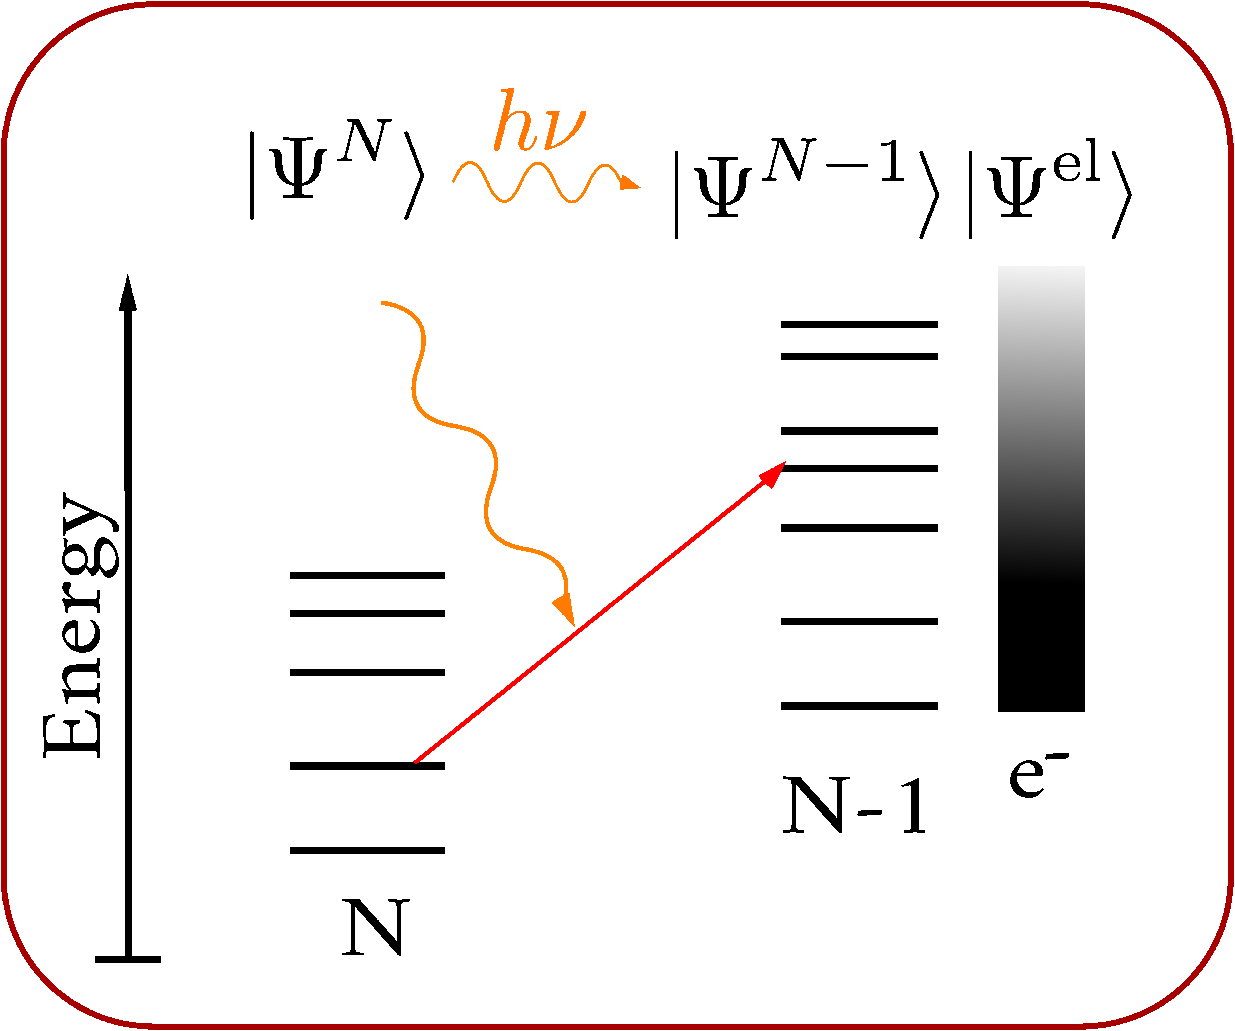
\includegraphics[width=0.61\textwidth]{Figures/PESscheme.eps}
   \caption{Schematic representation of a photoelectron transition : an incoming photon with energy $h\nu$ ionises the $N$-electron system, transferring it into a free electron in a continuum state and a system of $N-1$ bound electrons.
   The horizontal bars denote bound states, the gradient-filled rectangle depicts the continuum of states of the outgoing electron.}
   \label{fig:PESscheme}
\end{wrapfigure}
Furthermore, photoelectron spectroscopy provides a more direct access to the energy levels than optical absorption and emission spectroscopy since the transition energies are obtained with respect to the vacuum level and no ``dark'' states occur in general due to different selection rules.
Finally, the ease of handling charged particles experimentally makes this method appealing, \textit{e.g.}, a good temporal resolution can be achieved by varying the path in the time-of-flight spectrometer.
Thus, besides its capabilities in steady-state spectroscopy, photoelectron spectra (PES) have become the standard tool in attosecond physics due to the naturally high energy of the ultrashort pulses which ionise the systems under investigation \cite{as1, as2, as3, as4, as5, as6}.
However, a limitation of photoelectron spectroscopy is that the short free path of electrons in condensed phases decreases the probe depth significantly and special care should be taken to ensure the reliability of the results in this case.

The PESs of molecular systems are in general rich of features and hence their interpretation requires support from theoretical methods.
This especially applies to systems with strong electron correlation which manifests itself in the appearance of combination transitions.
Over decades a large variety of methods to calculate PESs has been developed at different levels of theory.
In literature, the theoretical spectra are often estimated on the basis of Koopmans' theorem \cite{koopmans}, (or its density functional theory (DFT) counterpart \cite{koopmansDFT},) assuming equal intensities for all transitions \cite{OT-RSH,Koerzd1,Koerzd2,Gao_wopperer}.
Although this is a quite successful approach for solid state \cite{Solid2,Leckey1992} and gives an easy interpretation, it is too simplistic in many cases since it neglects electron relaxation and correlation effects. 
Hence may it may give an invalid picture as shown by Cederbaum \textit{et al.} even for small systems such as various diatomics \cite{2phcederbaum2, cederbaumN2}.
Furthermore, in this model no reliable information about intensities can be obtained.
To retrieve quantitative  transition strengths, more advanced models are needed.
Since simulations in time domain are very demanding, they are only applied to small molecules, mainly to study strong-field effects such as high harmonic generation \cite{H2pDeCleva,as2,hhg, zhangHHG,dromey_HHG} which can not be described in frequency-domain.
In this thesis, however, the focus is put on complex molecular systems and a wide range of kinetic energies, while more moderate field strengths should be applied.
Hence frequency-domain methods derived from a perturbation theory with respect to the irradiating electromagnetic field are applicable here.

In present work, the PESs are calculated within the Dyson orbital (DO) formalism which is derived and explained in detail.
This formalism is based on Fermis' Golden Rule \cite{fgr} and allows a reduction of the dipole transition matrix element from an $N$-electron integral to effective one-particle quantities. % each for initial and final state.
Thereby the initial state and the bound part of the final state are represented by a one-electron quantity denoted as DO.
The other wave function entering the dipole moment operator is the free electron function (FEF).
In this formalism, electron relaxation and correlation effects between bound states of the unionised and ionised systems are included, allowing for the description of combination transitions.
Per contra, this formalism neglects the correlation of the outgoing electron with the ionic remainder and thus may neglect certain interchannel interaction effects \cite{LiSonntag}.

Since the bound state wave functions can be obtained from standard quantum-chemical tools, the computation of the DO is straightforward but practically demanding \cite{MAgg}.
The computation of the FEF is in general not trivial since analytic solutions are known only for few special cases such as hydrogen-like atoms \cite{Lifschitz} and localised Gaussian basis sets as they are used for bound states are not widely applicable.
Among others, three analytic expressions have been suggested, each based on an expansion of spherically symmetric functions in plane waves \cite{ezDyson}.
One of them is the spherical wave basis which is a set of solutions of the Schr\"odinger equation (SE) without any potential and hence is especially well-suited for photodetachment from negative ions, leaving systems in an uncharged state \cite{ezDyson, DO_TDDFT}.
The other two expansions are based on Coulomb waves which assume a spherically symmetric Coulomb potential and hence are exact for the ionisation of hydrogen-like atoms \cite{Lifschitz}.
Thereby one of them is an expansion in Coulomb waves for the given momentum vector $\vec{k}$ while the other is an asymptotic expression for Coulomb waves with vanishing momentum (Coulomb $|\vec{k}|=0$).
The FEFs are expanded in a series of waves with increasing quantum numbers for angular momentum $l$ and its projection $m$.
Since all three functions assume spherical symmetry of the potential, they are expected to give a good approximation to the real FEF for spherically symmetric systems only.
Ionisation, \textit{e.g.}, from a delocalised orbital of a linear molecule thus can be expected to be described only approximately by this approach.
%However, the more the system under consideration differs from spherical symmetry, the larger angular momenta are needed to describe the correct FEF and hence the truncated expansion is expected to give only a poor estimate of the correct function.
The effects due to low molecular symmetry become especially important for low kinetic energies.
% because the interaction with the ionic remainder becomes strong in this case. 

To analyse the quality of a given expression for a FEF, it is instructive to study the intensity of a given transition as a function of kinetic energy.
Such a dependence is exemplified in Figure \ref{fig:Ekin}, showing the intensity of the photoionisation transition from the highest occupied molecular orbital (HOMO) of water for different kinetic energies of the photoelectron, estimated with the above-mentioned expansions.
The comparison shows that all three expansions yield different intensities for most transition energies.
Besides leading to a wrong symmetry of the FEF, these expansions yielded even in the limit of infinite terms only a plane-wave, neglecting the ionic potential and hence are not asymptotically correct.

\begin{wrapfigure}{r}{0.62\textwidth}
   \includegraphics[width=0.61\textwidth]{Figures/water1}
   %\resizebox{\columnwidth}{!}{\input{Figures/water1}}
   \caption{The intensity of the transition with the lowest binding energy depending on the kinetic energy of the photoelectron exemplified for water molecule. Each wave expansion is performed up to $l_{max}=10$.} 
   \label{fig:Ekin}
\end{wrapfigure}
To overcome the restrictions in symmetry and kinetic energy of the photoelectron function, an explicit formulation is needed, taking the molecular electrostatic potential experienced by the outgoing electron into account.
%To account for the exact electrostatic potential, the final state needs to be treated as a full $N$ electron system to account for the correlation effects.
Assuming that the correlation between the FEF and the bound states of the ion is weak (which is a prerequisite for the DO formalism anyway), one can use the mean-field potential of the molecular remainder.
This allows for obtaining the FEF from the one-electron SE with an appropriate potential and thus considerably reduces the complexity compared to the exact case, where a coupled $N$-electron equation needs to be solved.

In this thesis, an approximation to the FEF is aimed which is applicable to a wide range of molecules and photon energies.
Such a flexible description is possible exploiting the finite element method for solving the SE.
In the finite element method, the space of interest is subdivided into small volume elements and solved variationally with stepwise polynomials whose support spans over one or few elements only \cite{femBraess,femGilbarg}.
The finite element description is especially efficient here since the size of the elements can be locally adapted to reproduce finer structures or broader shapes \cite{femBraess,femCiarlet}.
Using finite elements, the one-particle SE is formulated as a generalised eigenvalue problem with sparse matrices.

An important characteristic of the exact FEF is its spatially infinite extend which can not be handled by the finite element method.
To allow for this, the finite elements are extended by infinite elements \cite{astley3, astley2, Astley,dreyer} which are elements with infinite radial extent that are connected to the outer surface of the finite element region.
Thereby the radial function is a a plane wave $e^{ikr}$ multiplied by a polynomial of $\frac 1r$, resembling the asymptotic behaviour of known analytic solutions and fulfilling the Sommerfeld radiation condition \cite{sommerfeldCond}.

%The bound states can be obtained on the level of density functional theory (DFT) which is a formally exact method and yields a quadratic scaling with the number of electrons compared to the exponential growth of the SE \textcolor{green}{source}.
%The DFT is based on the Hohenberg-Kohn theorems \cite{HohenbergKohn}, stating that the total electron density contains all information to obtain any system property.
%However, the correct form of the exchange potential as well as the kinetic energy are not known therein and hence approximate functionals need used.
%While the kinetic energy can be estimated reasonably by the Kohn-Sham scheme \cite{KohnSham}, the expressions used for the exchange-correlation potential yield electron densities that have a wrong long-range asymptotic behaviour which affects the observables of these systems \cite{Koerzd1, Koerzd2, Bokareva}.
%To reduce this error, range-separated hybrid functionals are used where the usual DFT exchange functionals are used at close distances while a Hartree-Fock exact exchange ensures the correct behaviour at larger distances.
%Thereby the interchange between these contributions is modelled via an error function with a characteristic distance that is optimized for each system separately.
%This procedure has been observed to enhance the accuracy of the predicted properties such as the orbital energies \cite{Bokareva,GrellKuehn, Gerber, Gerber2}.
The bound states can be obtained on the level of density functional theory (DFT) which is a formally exact method based on the Hohenberg-Kohn theorem \cite{HohenbergKohn}, stating that the total electron density determines all system properties such as electronic binding energies.
However, the correct form of the exchange potential as well as the kinetic energy are not known as functionals of the electron density and hence approximate functionals need to be used.
Whereas the kinetic energy can be estimated reasonably by the Kohn-Sham scheme \cite{KohnSham}, the expressions used for the exchange-correlation potential yield electron densities that have a wrong long-range asymptotic decay which affects the computed observables \cite{Koerzd1, Koerzd2, Bokareva}.
To reduce this error, range-separated hybrid functionals are used where the usual DFT exchange functionals are used at small distances while a Hartree-Fock exact exchange ensures the correct behaviour at larger distances.
The interchange between these contributions is modelled via an error function with a characteristic distance that is optimized for each system separately.
This procedure has been observed to enhance the accuracy of the predicted properties such as the orbital energies \cite{Bokareva,GrellKuehn, Gerber, Gerber2}.

While the schemes described above are more or less well-established separately, their combination represents the novelty of the present work.
%Especially the FEF is found in literature to be approximated only crudely as plane-wave functions \cite{planeWave} or in some expansion as described above \cite{ezDyson,MAgg,GrellKuehn}.
This thesis unites three approaches: i) the DO formalism, ii) the description of the bound states by (TD)DFT using the above-mentioned optimized range-separated hybrid (OT-RSH) functionals to obtain accurate orbital energies, and iii) computation of a FEF that accounts for the molecular electrostatic potential either approximately via employment of Coulomb waves or explicitly using the finite and infinite element methods, which have been to date applied only to very few quantum-mechanical problems \cite{sobaMolecule,bettessHarmonic}.

%The Dyson formalism is well established and has been shown to give reasonable quantitative agreement with experiment for many different systems \cite{ezDyson,DO_TDDFT,bawagan,hafied}.
%In the protocol used the DO is calculated using density functional theory (DFT) and its time-dependent counterpart with a locally modified version of \prog{NWChem} \cite{nwchem} and the \prog{Gaussian 09} package \cite{g09}.
In the protocol used, the DFT and time-dependent DFT calculations for excited states are done using a locally modified version of \prog{NWChem} \cite{nwchem} and the \prog{Gaussian 09} packages \cite{g09}.
From those, the DO is calculated with the in-house code \prog{DYSON} developed previously \cite{MAgg}.
A self-written interface extracts the required data as \textit{e.g.} the molecular orbital coefficients and overlap matrix of atomic orbitals from the output of these programs.
For the computation of the FEF, the program \prog{FreeWilly} \cite{FreeWilly} is developed using the finite element library \prog{Libmesh} \cite{libmesh}. 
It is an open source library that provides a broad range of capabilities and interfaces to several high-performance linear algebra libraries \cite{slepc1,slepc2,petsc}.
Moreover, it supports MPI parallelisation and implements a recent formulation of the above-mentioned infinite elements \cite{dreyer}.
Especially the latter is, to the best of my knowledge, a unique option.
Furthermore, it has an automated procedure to adaptively refine or coarsen the elements according to local error estimations.
%
%Tho goal of this thesis is to find a systematic way to setup the finite element mesh for any given molecule to describe the photoelectron with a reasonable accuracy that goes beyond the capabilities of existing programs in this field.
%Moreover, the molecular electrostatic potential is to be obtained in the region of interest, requirering some modification in the code of \prog{NWChem} and a three-dimensional interpolation scheme that can handle nonuniform data.
%Finally, to obtain the dipole matrix elements, the DO has to be projected onto the space of finite elements.
%Therfore the explicit function is obtained by evaluating the basis functions at given quadrature points.
The developed protocol is applied to valence PES of two atomic (hydrogen and lithium) and two molecular (carbon dioxide and benzene) systems.
%To show the properties of the respective setup and compare different schemes suggested, atomic hydrogen is used for which an analytic solution, namely the Coulomb waves, is known.
%Further tests are applied to lithium, \textcolor{red}{doing .... and Cross section}.
%As a simplet test-system for a molecular case  carbondioxide is chosen for which several experimental as well as theoretical reference-data are available, \textcolor{red}{studying the PES and croos section}.
%For this system, the usual approach to represent the FEF as a Coulomb wave is expected to be not valid.
%Finally, as a representative for larger and more complex molecules, here benzene is chosen which is a well-studied system.


\chapter{Calculation of Photoelectron spectra}
%lit. survey I
The large variety of systems and effects studied with photoelectron spectroscopy lead to diverse methods \cite{PESbook, x-ray}.
In this work the interest is in steady-state photoelectron spectra of molecular systems with a size up to some tens of atoms.
As light source a classical ultra-violet or soft X-ray source is assumed as \textit{e.g.} discharge lamps based on helium, hydrogen, mercury or similar gases.
%Hence the strength of the applied electromagnetic field is considered as weak and the kinetic energies of the outgoing electrons reach to at most tens of electron volt but can become arbitrarily small.

However, besides this scenario, in the literature a large diversity of systems, studied with different inquests using photoelectron spectroscopy, is found.
Hence a large variety of models for the description of the PES is available, differing in the numerical effort but also in the assumptions and approximations implied.
These methods can be categorised as time- and frequency-domain approaches.
{\begin{table}
\begin{small}\begin{tabular}{|c|c|c|c|c|c|}
\hline
                 &  System Size & Typical Problems & Field Str. & QC & Formalism \\
\hline
\begin{tabular}{c}Time-\\ domain  \end{tabular}    &
        \begin{tabular}{c}atomic, \\ diatomic,\\ triatomic \end{tabular} & 
        \begin{tabular}{c}HHG, \\Multiph. ionisation \end{tabular} & strong & 
        \begin{tabular}{c}(TD)DFT, \\GASCI, \\CASSCF \end{tabular} &
        \begin{tabular}{c}  Time-dep. DO \\ SE \end{tabular} \\
\hline
\begin{tabular}{c}Frequency-\\ domain \end{tabular} & 
        \begin{tabular}{c}up to \\biomolecules \end{tabular}& 
        \begin{tabular}{c} steady-state, \\ time-res. PES, \\solid states, \\... \end{tabular}& weak & 
        \begin{tabular}{c}EOM-CC,\\ RASSCF, \\TD-DFT \end{tabular}&
        \begin{tabular}{c} R-Matrix \\ DO \\Greens' Function \\ Koopmans' \end{tabular} \\
\hline
\end{tabular} \end{small}
\caption{Overview of the capabilities of time- and frequency-domain methods.}
\label{tab:PEScat}
\end{table} 
As the Table \ref{tab:PEScat} shows, the time-domain methods are restricted to small systems which is due to the fact that the $N$ electron problem needs to be solved for every time-step and hence several hundred times per simulation.
In contrast to this, frequency-domain methods require only one solution and thus are much more efficient. 
However, the neglect of the nonlinear response properties make these schemes inappropriate when multiphoton ionisation and high harmonic generation (HHG) come into play.
%These nonlinear effects however usually do not play any role for classical light sources such as gas discharge or heat lamps and even most non-pulsed lasers.

Among the the frequency domain methods, the most prominent representative is the method denoted as Koopmans' approach in Table \ref{tab:PEScat} \cite{Koerzd1,PottsHolland,dos,dos2}.
In this scheme, the systems ground state is computed with a given quantum mechanical method to obtain the electronic binding energies.
The photoelectron spectrum is than estimated using the orbital energies as the transition energies and using uniform intensities.
While this method has shown to be at qualitatively in good agreement with experiment for some systems \cite{Koerzd1,Koerzd2, EggerKronik,PottsHolland,YepesJaque}, 
it breaks down in cases of strong electron correlation \cite{2phcederbaum,2phcederbaum2} due to strong changes in the orbitals upon ionisation.
%Since the estimation of the role of correlation effects can only hardly be estimated in advance, this method has only poor predictive character.
This method is characterised by its low computational costs and robustness and thus well-suited for very large systems such as solid states where calculations beyond ground-state DFT are very demanding on not feasible at all.

\begin{wrapfigure}{r}{0.7\textwidth}
   \includegraphics[width=0.7\textwidth]{Figures/Methods}
   \caption{Scheme of the system-representation used in the different methods.}
   \label{fig:PEScat}
\end{wrapfigure}
While in the Koopmans' approach only the ground state of the un\-ion\-ised state is considered, other methods treat the system under study in different ways.
In Figure \ref{fig:PEScat} the model of the system used the most important methods is schown schematically.
In a similar way as the Koopmans' theorem takes only the initial state into account, the Greens' function approach is implicit on the photoelectron.
A short introduction to this approach is given in section \ref{ch:gf}.
Among those methods that treat all $N$ electrons both in the initial and final state is a large group of methods where the photoelectron is treated on the same footing.
Out of this class, several approaches both in time- and frequency-domain are described in section \ref{ch:r-mat}.
Finally the Dyson orbital formalism describes the full $N$-electron system in the final state but here the photoelectron is treated separately, neglecting correlation effects with the bound states.
A more detailed derivation of the expressions used in this formalism is given in section \ref{ch:do}.

\section{The Greens' Function Approach}
\label{ch:gf}
In contrast to most other quantum-chemical methods, in the Greens' function approach expectation values for a given operator $\hat{O}$ are not computed as a scalar product $\langle \Psi^N |\hat{O} | \Psi^N \rangle $ with the wave function $|\Psi^N\rangle$ of the $N$ electron state of interest, but by contour integrals with the Greens' function \cite{bookGF, 1pGFcederbaum}.
Thereby the (one particle) Greens' function is a matrix $\mat{G}$ whose elements are defined as
\begin{equation} \label{eq:defGF}
G_{j,k}(t,t')= -\text{i}\langle \Psi^N | \hat{T}\left(\hat{a}_j(t)\hat{a}_k^\dagger(t')\right)|\Psi^N\rangle 
\end{equation}
with the creation operator $\hat{a}^\dagger_j (t)=e^{\text{i}\hat{H}t}\hat{a}^\dagger_j e^{-\text{i}\hat{H}t}$ of an electron in state $j$ at time $t$ in Heisenberg picture and the annihilation operator $\hat{a}(t)=e^{-\text{i}\hat{H}t}\hat{a}_j e^{\text{i}\hat{H}t}$ respectively.
$\hat{T}$ denotes is the Dyson time ordering operator that orders the operators $\hat{a}$ and $\hat{a}^\dagger$ by their time arguments to ensure that the operator with smaller time argument is on the right hand side of the other one \cite{bookGF}.
Hence, the Greens' function can be interpreted as an additional electron (or hole, depending on the time ordering) propagating from $t'$ to $t$ in a system described by the Hamiltonian $\hat{H}$ \cite{bookGF}.

In this approach the calculation of photoelectron spectra is formulated such that the poles and residues of the Fourier transformed Greens' function are searched.
This becomes clear when writing the time-ordering operator in equation (\ref{eq:defGF}) explicitly
\begin{equation} \label{eq:GF}
G_{j,k}(t,t')= -\text{i}\langle \Psi^N | \hat{a}_j(t)\hat{a}^\dagger_k(t') |\Psi^N\rangle \Theta(t-t') -
                   \text{i} \langle \Psi^N | \hat{a}^\dagger_k(t')\hat{a}_j(t) |\Psi^N\rangle \Theta(t'-t).
\end{equation}
Inserting the closure relation $\hat{1}=\sum_k |\Psi^M_k\rangle\langle \Psi^M_k |$, where $M=N\pm 1$ and $|\Psi^M_k\rangle$ describes a bound state, between the operators in both terms of (\ref{eq:GF}) the Lehmann representation \cite{bookGF} is obtained whose Fourier transform is
\begin{equation}\label{eq:gfSpect}
G_{j,k}(\omega)=-\text{i} \sum_k\frac{\left|\langle \Psi^N | \hat{a}_j|\Psi^{N+1}_k \rangle \right|^3}{\omega-(E_k^{N+1}-E^N)+\text{i}\nu}-
                \text{i}\sum_k\frac{\left|\langle \Psi^N | \hat{a}^\dagger_k|\Psi^{N-1}_k \rangle \right|^2}{\omega+(E_k^{N-1}-E^N)-\text{i}\nu},
\end{equation}
where $\nu$ is a small parameter arising from calculation of principal value.
Further $\omega$ denotes the argument of the Fourier transform while $E^N$ and $E_k^M$ are the energies of the $N$-electron ground stated $|\Psi^N\rangle$ and of the $k$-th $M$-electron state $|\Psi_k^M\rangle$ respectively.
In this form, the second sum corresponds to transitions in the photoelectron spectrum: the nodes of the denominator (poles of the Greens' function) can be easily assigned to the ionisation potentials and thus the transition energies in photoelectron spectra.
Further, the integrals in the nominator are equivalent to the sudden approximation derived in chapter \ref{ch:sa} and hence provide a good approximation to the transition strengths.
The terms in the first sum correspond to the respective quantities of electron detachment \cite{1pGFcederbaum}.

However, computing the Greens' function is a demanding task which is of similar complexity as the computation of a solution to the SE.
Over the years several approaches were developed of which the algebraic diagrammatic construction \cite{1pGFcederbaum} and the equation of motion \cite{PottsHolland,1pGFcederbaum} are the most prominent.
In the diagrammatic construction one starts with an initial zeroth order Greens' function $\mat{G}^0(\omega)$ constructed in a Hartree-Fock basis and corrects it iteratively by $\mat{G}^0(\omega)\mat{\Sigma}(\omega)\mat{G}(\omega)$, where $\mat{\Sigma}(\omega)$ is the self-energy, an effective potential that is used to recover electron correlation and relaxation effects \cite{GreenBayse}.
The self-energy usually is expanded in a perturbation series with respect to Feynman diagrams with increasing number of vertices and is exact in the limit of infinite terms \cite{bookGF,cederbADC}.
The one-particle energies, Coulomb matrix elements and overlap integrals are obtained from self-consistent field (SCF) calculations \cite{1pGFcederbaum} which are usually obtained on the HF-level \cite{GreenBayse} but (TD)DFT or any other quantum chemical method can be used as well \cite{Koerzd1}.
While being much easier to compute, the Hartree-Fock basis has the disadvantage that only single configurational electronic states can be treated.

On the other hand, an important advantage of the Greens' function method is that the transition energies are computed directly while in most other methods calculated it as the difference of the initial and final state functions.
The latter approach however can lead to errors in the electron volt range when the interaction energies are badly estimated \cite{1pGFcederbaum}.

%Another, yet similarly simple approach used in cases where only few electronic transitions are present is to fit the intensity to experimental data \cite{winterWater,hemberg1}.
%This is especially used when the vibrational structure is resolved.
%
%Here, two different approaches are possible.
%While most methods use Fermis Golden Rule 
%\[  \sigma(\omega)\propto |\langle |\hat{mu}|\rangle|^2 g(E_f-E_i+h\nu -\omega)
%\]
%where the intensity of the transitions is calculated via the dipole matrix elements, the other route is
%via the complex polarisability $\alpha(\omega)=\int_{IP}^\infty \frac{df(\epsilon)}{\epsilon^2-\omega^2}$. 
%In the latter case, the spectrum is obtained via
%\[ \sigma(\omega)=\frac{4\pi \omega}{c} Im(\alpha(\omega)).\]
% Some of them are especially generated for special geometries such as the R-matrix method described in chapter \ref{ch:r-mat}, others such as the Greens' function or Dyson orbital formalism introduced in the chapters \ref{ch:gf} and \ref{ch:do} respectively are more general but can not reach the same accuracy.
% Besides different classes of molecules, also the light irradiation considered can differ: Some methods are especially designed for large intensities \textcolor{green}{sources} or kinetic energies in the relativistic regime \textcolor{green}{source}.
 %In this work, however, only methods applicable in more moderate regimes are considered, meaning that perturbation theory is applicable and the kinetic energy of the photoelectron is considered to not above the $keV$-range.
%\section{Methods where electron is treated in same footing as bound states}
%\section{Methods with Unified Description of Bound and Free States}
\section{Combined Bound and Continuum State Representation}
\label{ch:r-mat}
%Another large class of methods for computing photoelectron spectra uses perturbation theory in frequency domain or the dipole autocorrelation function in time domain respectively.
%In frequency domain thereby the initial state and final state are described therein each as $N$ electron systems with a uniform scheme, requiring the basis set to be formulated general enough to represent bound as well as free states.
In contrast to the Greens' function method in which the explicit description of the FEF  omitted, a large group of methods describes the full $N$-electron system before and after the ionisation respectively.
With this approach electron correlation effects also between bound and unbound states are accounted for but a large and flexible basis is required which can represent bound as well as unbound states of electrons.
Due to this, these methods are generally restricted to small systems that fulfil certain symmetry-requirements and have only a low amount of electrons.

The most prominent representative of this class in frequency-domain is the R-matrix method \cite{r-mat, r-mat2,Burke}.
Its general idea is to conduct a partition of space into regions which are treated differently, connected by explicit boundary conditions to ensure smoothness of the wave function.
These regions are constructed with concentric spheres, restricting the symmetry of wave functions in this scheme.
Nonetheless it is applied not only to atoms \cite{Li-R,Li-R1,Li-R2} but also to small molecules \cite{R-mol1,R-mol2}.
\begin{wrapfigure}{r}{0.48\textwidth}
   \includegraphics[width=0.48\textwidth]{Figures/JohnsonSpheres}
   \caption{Schematic view of the space partition scheme used by Johnson for a four-atomic molecule:
    I: atomic, II: interatomic and III: extra-molecular space \cite{johnson}.}
   \label{fig:johnson}
\end{wrapfigure}
In the R-matrix formalism the inner region is chosen large enough to contain the bound part of the $N$-electron function that is usually represented by a configuration interaction (CI) expansion of Slater determinants (SDs), using a with a linear combination of atomic orbitals (LCAO) basis or a grid representation \cite{Burke}.
The FEF commonly is described by a linear combination of bound orbital type functions and continuum functions such as Coulomb waves \cite{r-mat, r-mat2}. %or a product description of spherical Harmonic and a spline-based radial function.
%a antisymmetrised product of Coulomb type wave function with ...\cite{r-mat,r-mat2}.
In the outer region, an expansion in Coulomb waves is used to ensure the asymptotically correct behaviour.
In addition to the inner region, where correlation plays an important role, and the asymptotic outer region further intermediate regions can be added  where the FEF is represented by a multipole-radiation expansion which is a polynomial of inverse powers of the distance to the centre \cite{Burke}.

%in which the multipole functions can be added\cite{Burke}.
A generalisation to non-spherical systems is employed, \textit{e.g.}, by Johnson \cite{johnson} who used different kinds of non-concentric spheres.
One set of spheres is centred each at an atom while others are placed such in the interatomic regions such that the space is filled as dense as possible as shown in Figure \ref{fig:johnson} for a molecule with four atoms.
Each atom is located in the centre of a circle denoted as I while the circles II fill the interatomic space.
An outer sphere surrounds the molecule to account for the asymptotic region similar to that used in R-matrix theory.
In this scheme the exchange-correlation is treated on an approximate level \cite{slaterJohn} and is spherically averaged, resulting in a description that is equivalent to the muffin-tin potential which is a well-known model in solid state physics \cite{MufTin,MufTin1}.
The continuity of the wave-functions as well as their derivatives is a ensured over the regions using multiple-scattered-wave theory \cite{johnson}.
%Thereby the potential energy contains besides the Coulomb term also a statistical approximation of the exchange correlation of the form
%\begin{equation}
 %V_{x\alpha}(\vec{r}) = -6\alpha\left( \frac 38 \pi \rho(\vec{r})\right)^{\frac 13} 
%\end{equation}
%where $\rho(\vec{r})$ is the electron density and $\alpha$ is a parameter that is chosen differently for each element.
%In each of the regions the potential %energy is expanded in a superposition of spherical harmonics that is truncated after the $l=0$ term which is equivalent to the muffin-tin potential which is well-known especially for solids \cite{MufTin,MufTin1}.
The wave-functions are chosen in each region as a one-centre expansion of the form
\begin{equation} \label{eq:radSE}
\Psi(\vec{r})=\sum_{l=2}^{l_\text{max}}\sum_{m=-l}^l c_{l,m} R_l(r) Y_l^m(\theta, \phi)
\end{equation}
where $r,\theta,\phi$ are the coordinates of the spherical coordinate system and $Y_l^m(\theta,\phi)$ are the spherical Harmonics \cite{Lifschitz}.
The radial function $R_l(r)$ solves the radial SE 
\begin{equation}
\frac{\partial^2 R(r)}{\partial r^2} + \left( E-V(r) + \frac{l(l+1)}{r^2} \right)R(r)=0
\end{equation}
with the respective spherically averaged potential $V(r)$ \cite{johnson}.

%A similar approach is to describe the bound and free states at the same level as applied by DeCleva \textit{et al.}  $H_2^+$\cite{H2pDeCleva}.
An approach applied by DeCleva \textit{et al.} to $H_2^+$ \cite{H2pDeCleva} and benzene \cite{DeClevaBenzene} resigns the use of spheres, allowing for more general boundaries between the inner and outer regions.
Here the FEFs are globally described in the one-centre expansion (\ref{eq:radSE}) where $R(r)$ is described by a B-spline basis. % (details about the spline description are given in section \ref{ch:dvr}).
The advantage of the spline-based description is that smoothness at the interface of the regions is ensured intrinsically.

Another scheme in frequency domain is used by Richards and Larkins \cite{richardsFD} with a hybrid ansatz: While the bound states of the H$_2$ molecule are described in the common LCAO scheme, the FEF is described by the product ansatz $\Psi(\vec{r}) = R(r,\theta) e^{im\phi}$ where $R(r,\theta)$ is obtained on a two-dimensional grid using a finite difference (FD) scheme.
In contrast to the previously described methods, here no partition of space is conducted but instead a finite box with Dirichlet boundary conditions is used.
Moreover, the FEF is treated on the HF-level, neglecting correlation effects \cite{richardsFD}.

Similar descriptions are used in time-domain by several authors \cite{CAPccEOM, bauch1, taoDVR}.
Since a time-domain description requires the recomputation of the $N$-electron function for each time-step and thus several hundreds to thousands of times per simulation, its computational effort is increased by far.
On the other hand, time-domain methods allow the description of non-linear effects such as high harmonic generation and multi-photon ionisation \cite{as2} which are both not perceptible by frequency-domain methods.

An important difference between time- and frequency-domain methods of practical means is that in time-domain free particles are described by a wave packet and hence as a localised function.
Moreover, at short times after ionisation the continuum states often can be assumed to be coupled diabatically to the bound states (\textit{i.e.} the wave packet does not move away from the ionic remainder).
Under this assumption, the spacial part of the FEF can be written as a linear combination of bound state functions but having a complex energy that determines the oscillations and finite lifetime of the function \cite{CAPccEOM}.
Moreover a complex absorbing potential (CAP) (discussed in chapter \ref{ch:cap} in more detail) is most often applied, ensuring the assumption of diabatic coupling to the bound states by cutting off that part of the wave function which is not localised at the molecule anymore.
Due to these considerations the LCAO basis can be used here for the description of the free particles as well, as conducted \textit{e.g.} by Jagau \textit{et al.} \cite{CAPccEOM}.
In other simulations, grid-based descriptions are chosen using symmetry-adapted coordinate systems \cite{radau,jacobi, hyperspheric,taoDVR}, allowing a product ansatz and hence a reduction in dimensionality.
%In other simulations, a grid-based description is chosen using spherical, elliptical or hyperspherical coordinates, allowing ng for a product ansatz and hence a reduction to one dimension.
On the remaining one-dimensional grids often a discrete variable representation (DVR) (described in section \ref{ch:dvr} of this thesis) is chosen.
As an example, Yip \textit{et al.} \cite{yipDVR} simulate double ionisation of atomic beryllium in spherical coordinates, using the expansion (\ref{eq:radSE}) where $R(r)$ is separated into two regions in which a DVR and a finite element DVR (FE-DVR) scheme are used respectively.
Tao \textit{et al.} \cite{taoDVR} as well as Bauch \textit{et al.} \cite{bauch1, bauch2} use the FE-DVR basis in spheroidal coordinates respectively.

\textcolor{red}{This is by far not a complete list; are these at least the most important methods?}

%A different technique is used by Son \textit{et al.} who use time dependent density functional theory (TDDFT) based on a finite volume scheme instead of the usual LCAO approach.
%Thereby no asymptotic region is utilised, instead the region of interest is chosen by setting a sphere with a given radius around each atom \cite{Son_Chu0,Son_Chu}.

%Sato \textit{et al.}\textcolor{green}{sources} 
\section{The Dyson Orbital Formalism}
\label{ch:do}
The Dyson orbital (DO) formalism can be considered as an approximation to the formalisms described above where the free and bound states are described separately.
Using such a separation leads to an neglect of correlation effects between the outgoing electron and the bound states and is often denoted as sudden ionisation limit \cite{ezDyson,MAgg}.
In this formalism the overlap between the initial state and the bound part of the final state is formulated as an effective one-electron quantity, called DO.
%reducing the computation of the dipole matrix elements to a one-electron integration.
Usually the DO scheme is considered in the frequency domain, but a time domain formulation exists as well and is described in the following subsection \cite{TD-do}.
%The DO therein can be interpreted as a quasi-particle that is removed from the molecules; incorporating multi-particle effects such as electron relaxation or instantaneous excitation of other electrons.

\subsection{Time-dependent Dyson Orbitals}
%There are several approaches towards Dyson orbitals.
%Here we will mainly follow the derivation of Gritsenko \textit{et al.} \cite{TD-do}, starting from an exact time-dependent expression.
%Here we will mainly follow the derivation of Gritsenko \textit{et al.} \cite{TD-do}, starting from an exact time-dependent expression.
%Thereby the $j$-th time dependent Dyson orbital (TDDO) is defined as the overlap integral of the $j$-th final ionised state $\Psi_j^{N-1}^\dagger(\vec{r}_2,\hdots,\vec{r}_N)$ with the unionised initial $N$-electron state $\Psi^{N}(\vec{r}, \vec{r}_2,\hdots,\vec{r}_N)$
%\begin{equation}
%\Psi_\text{DO}^j(\vec{r}) = \sqrt{N} \int \Psi_j^{N-1}^\dagger(\vec{r}_2,\hdots,\vec{r}_N)
%                                           \Psi^{N}(\vec{r}, \vec{r}_2,\hdots,\vec{r}_N)
%                            d\vec{r}_2 \hdots d\vec{r}_N .
%\end{equation} 
A good starting point for the DO formalism is an expansion of the time-dependent $N$-electron function $\Psi^N(\vec{r}, \vec{r}_2, \hdots,\vec{r}_N, t)$ in the form
\begin{equation} \label{eq:DOexpansion}
%\Psi^N(\vec{r}, \vec{r}_2, \hdots,\vec{r}_N, t)=\frac{1}{\sqrt{N}} \sum_k \Psi^k_\text{DO}(\vec{r},t) \Psi_k^{N-1}(\vec{r}_2, \hdots,\vec{r}_N)e^{\text{i}E_k^{N-1}t}
| \Psi^N (t)\rangle =\frac{1}{\sqrt{N}} \sum_k |\Psi_k^{DO}(t)\rangle | \Psi^{N-1}_k \rangle e^{iE_k^{N-1}t}
\end{equation}
where $E_k^{N-1}$ are the energies of the $N-1$-electron bound states described by the wave functions $|\Psi_k^{N-1}\rangle$ that are complete in the space of $N-1$-electron wave-functions.
The expansion coefficients $|\Psi_k^{DO}(t)\rangle$ have the dimensionality of a one-particle function and are denoted as the time-dependent DO (TDDO).
An important feature of the expansion (\ref{eq:DOexpansion}) is that the dynamics of the $N$-electron system are reduced to a system of one-electron quantities $|\Psi_k^\text{DO}(t)\rangle$ propagated by a TDDFT-like equation of motion \cite{TD-do}.
\textcolor{red}{Put the EOM here?}
%\begin{equation}
%\text{i}\frac{\partial}{\partial t}|\Psi_j(t)\rangle =
%\left{-\frac 12 \nabla^2 + \hat{v}_\text{ext}(\ver{r},t) +\Delta_j(t) \right} |Psi_j(t)\rangle
%\end{equation}
In this approach the interaction of the DO with the bound states is approximated by the mean-field electrostatic potential \cite{TD-do}, neglecting exchange and correlation.

The physical interpretation of the DO becomes clear when regarding its definition, given by
\begin{equation} \label{eq:TDDO}
%\Psi^k_\text{DO}(\vec{r},t) = \sqrt{N} \int \Psi_k^{N-1 \dagger}(\vec{r}_2,\hdots,\vec{r}_N) e^{\text{i}E_k^{N-1}t}
                              %\Psi^N(\vec{r}, \vec{r}_2, \hdots,\vec{r}_N, t) d\vec{r}_2,\hdots d\vec{r}_N.
|\Psi_k^\text{DO}(t)\rangle =  e^{\text{i}E_k^{N-1}t}\sqrt{N} \langle \Psi_k^{N-1} |\Psi^N(t) \rangle.
\end{equation}
The remaining coordinates not integrated in (\ref{eq:TDDO}) belong to the photoelectron since $|\Psi^{N-1}(t)\rangle$ is restricted to the description of bound states
Hence in a frozen orbital approximation the DO is identical to the photoelectron.
However, relaxation-effects change the overlap and thus lead to additional contributions to the TDDO.
These considerations suggest to interpret the TDDO as a quasi-particle describing the electron that is ionised, including relaxation and correlation effects \cite{ezDyson,TD-do}.
%Thereby especially three time slices are interesting: $t<0$ \textit{i.e.} before the ionisation , $t=0$ and the limit of $t\rightarrow \infty$.
%For $t<0$ hence the expression (\ref{eq:DOexpansion}) describes the unionised system in its initial state where the DO is a molecular orbital and equation (\ref{eq:DOexpansion}) is a way to write a Slater determinant (SD).
%In the limes of $t\longrightarrow \infty$ thereby $|\Psi_k^{N-1}\rangle$ describes the ionic remainder in a state $k$ and hence the TDDO is the free electron function (FEF) whose energy is determined by the laser pulse which ionised the system as well as the energy $E_k^{N-1}$.
%However, due to relaxation and correlation effects, the orbitals in the final states are different from those in the $N$ electron state and hence these changes are also contained in the TDDO.
%For the case $t=0$ these relaxation effects also are included in the TDDO but the FEF did not change its wave function with respect to the ionised orbital hence its wave function is that of the removed electron, amended by combination and relaxation effects. \\ \\
%Thereby, this formalism resolves two main problems of time propagation using standard TDDFT which are the missing memory effects due to an approximate exchange potential that depends on the current density only. % this is resolved because in the 1-particle EOMs only static electron-electron interaction potentials occur.
%The second problem often occurring is that usual TDDFT is not able to predict correlated multiple ionisations which can be resolved with this formalism as well \cite{TD-do}.

\subsection{Time-independent Dyson Orbitals}
Working in frequency domain, no propagation of the TDDO nor the ionised system (\ref{eq:DOexpansion}) needs to be considered.
The time-independent DO is defined rather as the TDDO at $t=0$.
Since at this point the FEF is coupled adiabatically to the respective orbitals, the DO can be interpreted as quasi-particle that is ejected by the irradiating light \cite{ezDyson}.

%To see the benefit of using the DO formalism for computing photoelectron spectra, we start with the photoelectron cross section in atomic units
The main advantage of this formalism in frequency-domain becomes clear when the photoelectron cross-section is considered.
In the Fermis' Golden Rule formulation, which assumes the wavelength to be much larger than the system under study and weak irradiating light-field, the cross-section is in atomic units \cite{richardsFD,MAgg}
\begin{equation} \label{eq:sigma}
\sigma(\epsilon) =\frac 23
           \nu \sum_k\left| \langle \Psi^N_i | \vec{\hat{d}} | \Psi^N_{k}\rangle
\right|^2  
             \propto \sum_k \left|  \vec{D}_k \right| ^2
\end{equation}
where $\epsilon=\nu-(E_k-E_i)$ is the kinetic energy of the photoelectron that is determined by the photon energy $\nu$ and the energies $E_i$ of the initial unionised state $|\Psi^N_i \rangle$ and the total binding energy $E_k$ of the final ionised state $|\Psi^N_k\rangle$ which includes all electrons.
Writing the initial and final states each as SDs
\begin{subequations} \label{eq:SDs} \begin{align}
   |\Psi^N_i\rangle &= \hat{A}_N | \Phi_{i,1} \hdots \Phi_{i,N} \rangle \\
   |\Psi^N_k \rangle &= \hat{A}_N | \Phi_{k,1}\hdots \Phi_{k,N-1} \Psi_k^\text{el} \rangle
\end{align}\end{subequations}
where $\hat{A}_N$ is an $N$-electron antisymmetrisation operator.
Furthermore the one-electron quantities $|\Phi_{k,j}\rangle$ denote the $j$-th (Kohn-Sham) orbitals and $\Psi_k^\text{el}$ is the FEF.
The index $k$ enumerates the final states which can have an arbitrary electron configuration here.
The dipole operator $\hat{\vec{d}}$ is a one-electron operator that can be written as$\hat{\vec{d}}=\sum_{j=1}^N \hat{\vec{d}}_j$ where $\hat{\vec{d}}_j=\vec{r}_j$ in length gauge or $\hat{\vec{d}}_j=\nabla_j/(2\pi\nu)^2$ in velocity gauge respectively \cite{richardsFD}.

Using the SD representations (\ref{eq:SDs}), the integral $\vec{D}_k$ in equation (\ref{eq:sigma}) can be written as
\begin{equation} \label{eq:derDO1}
\vec{D}_k = \langle
\Phi_{i,1}  \hdots\Phi_{i,N} | \hat{A}_N \sum_{j=1}^N\hat{\vec{d}}_j \hat{A}_N |
\Phi_{k,1}\hdots\Phi_{k,N-1} \Psi_\text{el} 
\rangle 
\end{equation}
where hermiticity of the antisymmetrisation operator is used.
The expression (\ref{eq:derDO1}) can be further expanded by commuting $\hat{A}_N$ with the dipole operator and making use of the relation $\hat{A}_N\hat{A}_N=\sqrt{N!}\hat{A}_N=\sum_P (-1)^p \hat{P}$ where the sum goes over all permutations $\hat{P}$ with parity $p$
\begin{align} \label{eq:derDO2}
\vec{D}_k & = \sqrt{N!}\sum_P (-1)^p \sum_{j=1}^N \langle
\Phi_{i,P(1)}\hdots\Phi_{i,P(N)} |\hat{\vec{d}}_j |
\Phi_{k,1}\hdots\Phi_{k,N-1} \Psi_\text{el}  \rangle  \\
  & = \sqrt{N!}\sum_P (-1)^p \sum_{j=1}^N 
  \langle \Phi_{i,P(j)} | \hat{\vec{d}}_j | \Phi_{k,j} \rangle
          \langle \Phi_{i,P(1)}  |\Phi_{k,1}   \rangle
  \hdots  \langle \Phi_{i,P(j-1)}|\Phi_{k,j-1} \rangle \\
  & \times\langle \Phi_{i,P(j+1)}|\Phi_{k,j+1} \rangle
          \langle \Phi_{i,P(N-1)}|\Phi_{k,N-1} \rangle
  \hdots  \langle \Phi_{i,P(N)}  |\Psi_\text{el}\rangle 
\end{align}
where $P(j)$ is a permutation of the $j$-th orbital.
Thereby the term $j=N$ differs qualitatively from the others since the dipole operator acts on the FEF.
Hence the sum can be reordered to obtain
\begin{align} \label{eq:fullDO}
  \vec{D}_k & = 
  \underbrace{\sqrt{N!}\sum_P (-1)^p 
          \langle \Phi_{i,P(1)}  |\Phi_{k,1}    \rangle
  \hdots  \langle \Phi_{i,P(N-1)}|\Phi_{k,N-1}  \rangle
  \langle \Phi_{i,P(N)} }_{\langle \Psi_k^\text{DO}|} | \hat{\vec{d}}_j | \Psi_\text{el} \rangle + \nonumber \\
  & 
       \sqrt{N!}\sum_P (-1)^p \sum_{j=1}^{N-1} 
          \langle \Phi_{i,P(1)}  |\Phi_{k,1}    \rangle
  \hdots  \langle \Phi_{i,P(j-1)}|\Phi_{k,j-1}  \rangle \times \nonumber \\
  &       \langle \Phi_{i,P(j+1)}|\Phi_{k,j+1}  \rangle
  \hdots  \langle \Phi_{i,P(N-1)}|\Phi_{k,N-1}  \rangle
 \langle \Phi_{i,P(j)}|\hat{\vec{d}}_j |\Phi_{k,j}\rangle
  \langle \Phi_{i,P(N)}| \Psi_k^\text{el} \rangle
\end{align}
where the first sum is denoted as DO and the second as conjugate DO respectively \cite{saPonzi}.
To reduce the large amount of integrals therein, the strong orthogonality approximation is applied under the assumption that the overlap 
\begin{equation}
 \langle \Phi_{k,j}  |\Psi_\text{el}\rangle=0 \quad \forall\, j=1,\hdots, N.
\end{equation}
of the FEF with all bound states vanishes.
This would be strictly valid if they would correspond to the same Hamiltonian.
But in most cases the orbitals of the ionised and unionised state are similar, leading to small but non-zero overlaps \cite{saPonzi,GrellKuehn}.
Applying the strong orthogonality condition leads to the drop out of the second sum in equation \ref{eq:fullDO} and the transition dipole moment simplifies to
\begin{align} \label{eq:sigma_do}
\vec{D}_k&= \sum_p (-1)^P \langle \Phi_{i,P(1)}  |\Phi_{k,1} \rangle
            \hdots  \langle \Phi_{i,P(N-1)}|\Phi_{k,N-1} \rangle
                   \langle \Phi_{i,P(N)} |\hat{\vec{d}}_j |\Psi_k^\text{el}\rangle \nonumber \\
    &= \langle \Psi_k^\text{DO}| \hat{\vec{d}}_j| \Psi_k^\text{el}\rangle
\end{align}
which corresponds to the definition of the TDDO in equation (\ref{eq:TDDO}) for $t=0$ as mentioned above.
The expression for the PES cross-section in the DO formalism simplifies to
%Though the cross section simplifies from the $N$ electron expression (\ref{eq:sigma}) to 
\begin{equation} \label{eq:DO_pes}
\sigma(\epsilon) =\frac 23 (\epsilon +E_k-E_i)
           \sum_k \left|  \langle \Psi^k_\text{DO} | \hat{\vec{d}} | \Psi_\text{el}\rangle  \right|^2 .
\end{equation}
In the derivation given here, it is assumed that initial and final state can be represented by a single SD each.
In practice, often states are described by a linear combination of SDs with different electron configurations.
A respective generalisation of the DO is straight forward but introduces additional summations and thus leads to more complex terms.

\subsection{Sudden Approximation}
\label{ch:sa}
Further simplification of the DO formalism can be obtained by applying the so-called sudden approximation (SA) where the computation of the FEF is avoided.
In the SA it is assumed that the transition to a continuum function with corresponding energy has a constant probability which can be justified by the high degree of degeneracy of continuum functions for each given energy.
Thus, the transition probability
\begin{equation}
\vec{D}_k= \sum_p (-1)^P \langle \Phi_{i,P(1)}  |\Phi_{k,1} \rangle
           \hdots  \langle \Phi_{i,P(N-1)}|\Phi_{k,N-1} \rangle
                   \langle \Phi_{i,P(N)}  |\hat{\vec{d}}_j |\Psi_\text{el}\rangle 
\end{equation}
reduces to 
\begin{equation} \label{eq:sa}
D_k= \sum_p (-1)^P \langle \Phi_{i,P(1)}  |\Phi_{k,1} \rangle
           \hdots  \langle \Phi_{i,P(N-1)}|\Phi_{k,N-1} \rangle
\end{equation}
which is the probability for the bound $N-1$-electron system to conduct the transition between the respective bound states of the unionised and ionised system \cite{saAberg}.
With this assumption the kinetic energy dependence of the PES is neglected, assuming error introduced is a similar factor for all transitions.
This has shown to be a valid assumption if the nature and spacial extend of the Dyson orbitals is similar.

Moreover, the expression (\ref{eq:sa}) corresponds to the nominator of the Greens' function in (\ref{eq:gfSpect}) and thus is the level of theory at which the Greens' function PES transitions are computed.

Finally, the expression (\ref{eq:sa}) can be further simplified to get the approach described in the introduction of this chapter, based on Koopmans' theorem.
Therefore the electron relaxation is neglected and thus the $N-1$-electron state can be written as $|\Psi_{k}^{N-1}\rangle= \hat{a}_k|\Psi_i^N\rangle$. 
Thus, the sum over all permutations $\hat{P}$ in (\ref{eq:sa}) reduces to the case where $P(j)=j\,\forall j=1,\hdots,N-1$ due to orthogonality of the orbitals.
Moreover, due to the normalisation of the orbital functions, all transitions have a probability of one and thus corresponds to the scheme described earlier.


\chapter{Description of Free Particles} 
% lit. survey II
The description of particles in continuum states bears several complications of conceptual and technical kinds.
%Some methods to obtain the FEF had been mentioned in section \ref{ch:r-mat} already, 
In this chapter different numerical methods are introduced that can be used to solve the one-electron SE.
In section \ref{ch:contwa} the conceptual differences between bound and continuum states as well as the numerical treatment of the latter in a finite basis are discussed.
Thereafter, in the sections \ref{ch:FD} - \ref{ch:wavelet} different numerical methods are introduced that can be used to solve the one-particle SE on a molecular domain.
%These methods can be roughly divided into two main classes: In section \ref{ch:FD} the finite difference and finite volume methods are introduces which both are based on the approximation of the operators by differences of function values.
%The other methods are based on different basis expansions wich are designed with different properties
%\textcolor{red}{Need to think a bit how to expand on this. Moreover: splines don't fit in there, do they? --> need further category?}
% based on finite differences, a basis-expansion of finite element.

\section{Continuum Waves}
\label{ch:contwa}
Continuum waves are discussed only sparsely in lectures on quantum mechanics, even though they posses certain properties of fundamental difference compared to bound states.
The states considered here have a spatially infinite extend as it is well-known for plane waves $\Psi(\vec{r})=e^{i\vec{kr}}$ as well as spherical waves. %whose radial part contains different powers of $\frac{\sin(kr)}{kr}$ \cite{Lifschitz}.
Morover, these waves are not square integrable and hence can not be normalised according to $\int \Psi^\dagger(\vec{r})\Psi(\vec{r}) d\vec{r}=1$ and so the probability interpretation is invalid \cite{quirky}.
Instead, these functions are sharp in a continuous variable (namely the momentum) and hence should rather be interpreted as probability densities, suggesting the normalisation 
$\int \Psi^\dagger(\vec{r})\Psi(\vec{r'}) d\vec{r}=\delta(\vec{r}-\vec{r'})$ where $\delta(\vec{r})$ is the Dirac delta distribution \cite{quirky}.
This property distinguishes the analytical FEF from those obtained from numerical methods that often have a finite extend and are obtained from an approximate Hamiltonian which has no continuous spectrum due to finiteness of its basis.
This difference in the dimensionality of the wave functions also affects the integral evaluated when calculating the transition dipole matrix elements \cite{stieltjesCeder}.
Nonetheless this problem can be resolved by the Stieltjes-Imaging approach described in the subsection \ref{ch:stieltjes}.
The Stieltjes-imaging technique moreover can be used to varify the use of a square-integrable function for the representation of a continuum state since it can be considered as $0$-th order moment expansion.

A second aspect that is only sparsely discussed in literature concerns the question of what the numerical solution corresponds to.
When dealing with approximate continuum functions, it is often assumed that the analytical function of interest $|\Psi_\text{a}(\vec{k})\rangle$ is approximated by that particular numerical solution $|\Psi_\text{n}(\vec{k}')\rangle$ which is closest in energy \cite{H2pDeCleva}.
An alternative interpretation would be to assume that the numerical solution corresponds to an approximation to $|\Psi_\text{n}\rangle \approx \frac{1}{k^+-k^-} \int_{k^-}^{k^+}|\Psi(k) \rangle dk$ which would change the interpretation and normalisation of the respective numerical solution.
%
%This rises the question, whether a numerically obtained free electron state corresponds most to the analytic state with the same kinetic energy, hence
%$\Psi\approx \Psi_k$
%or whether it should be considered more as an integration over a small part of the spectrum
%$\Psi\approx \frac{1}{k^+-k^-} \int_{k^-}^{k^+}\Psi(k) dk$
%which changes the interpretation and normalisation required for the wave function.

A further conceptual problem is due to degeneracy of the analytical solution.
This issue becomes apparent when considering the ionisation of a hydrogen-like atom whose analytical FEF is well-known and has the form
%
%In addition to the transition from a continuous to a discontinuous spectrum, also degerarcy plays an important role.
%This can be best discussed when taking the example of the ionisation process of a hydrogen atom where the corresponding FEF has the analytic form
\begin{equation} \label{eq:CoulWave}
\Psi_{\vec{k}}(\vec{r})=\frac{1}{(2\pi)^{\frac{3}{2}}}\frac 1r
\sum_{l=0}^\infty \sum_{m=-l}^l c_{l,m} w_l\left(\frac Zr,rk\right), Y_l^m\left(\theta, \phi\right) Y_l^m\left(\theta_k, \phi_k\right)
\end{equation}
where $Z$ is the change of the nucleus, $k=|\vec{k}|$ is the absolute value of the wave vector $\vec{k}$ and the arguments to the spherical Harmonics $Y_l^m$, $(\theta,\phi)$ and $(\theta_k,\phi_k)$, are the angles of the spherical coordinate system in real-space and Fourier-space respectively \cite{ezDyson}.
Finally $w_l\left(\frac{Z}{k}, rk\right)$ is the radial wave function that can be expanded in an infinite term of confluent hypergeometric functions \cite{Lifschitz}.

The function (\ref{eq:CoulWave}) is, given its energy $E=\frac 12 |\vec{k}|$, degenerate in the direction of $\vec{k}$ as well as in the quantum numbers $l$ and $m$ with infinite terms respectively.
Hence the wave function of a photoelectron can consist of any superposition of the form (\ref{eq:CoulWave}), chosing the coffecients $c_{l,m}$ accordingly.
The coefficients $c_{l,m}$ of the physically observable FEF are determined by the overlap integrals with the DO (\ref{eq:sigma_do}).  
Considering as an example the ionisation of hydrogen in its ground state, the FEF will allways be in one of the three $p$-waves because the probability to access any of the other vaccum-states with the correct energy vanishes. 

Unfortunately, the considerations made above are not true for the numerical solution anymore where a finite set of superpositions is obtaind which, due to numerical treatment, differ in energy and thus can not be assigned to a common value of $\vec{k}$.
Chosing the energetically best-fitting solution though might result in a function with vanishing contribution of the $p$-type orbitals while, for slightly changed paraters or target energy (or even just using an other computer) could yield a solution with large contributions with $l=1$.

%The coefficients $c_{l,m}$ moreover are arbitrary coefficients to this end since any of the linear combinations solves the SE for a given kinetic energy.
%Hence analytical the solutions are not only continuous in $\vec{k}$, but also infinitely degenerate in $l$ and $m$.
%In contrast to this, the numerical solution will be a linear combination of some of these terms; in the easiest case it is close to one of these $l$ and $m$.
%However, for the case of ionisation from the hydrogen ground state only the contributions with $l=1$ will lead to a transition probability; having a solution of $l=2$-character would lead to vanishing probability.
%Hence, the lifting of degeneracy would lead to intensities that are very sensitive to the kinetic energy of the photoelectron since the $l=1$ solution might be only few meV off that solution of $l=2$-type.
%Moreover, the numerical grid may influence this dependency since it could, by accident, supporting certain symmetries.
%
%A detailed discussion of the conceptual complications arising from this is not found in the literature.
%The FEF used to describe the ionisation of H$_2$ as discussed in \cite{H2pDeCleva} is chosen as that function which fits the target energy best.
%However, in their formulation this energy is well-separated from the others % (spline base without boundary conditions, leading to non-hermitian Hamiltonian). -> do they implicitly use some boundary conditions ?
%They also discuss formulation as minimisation problem: More stable but they don't need it.
%which will be later shown to be not the case here.

\subsection{Stieltjes Imaging}
\label{ch:stieltjes}
The Stieltjes imaging provides an elegant way to still use the numerially obtained solutions of a non-continuous spectrum by using moment theory.
Starting from the expression for the photoelectron spectrum 
\begin{equation}
\sigma(\varepsilon)\propto \left|\langle \Psi_0 |\hat{d}|\Psi_\text{el} \rangle \right|^2
\end{equation}
where $\Psi_\text{el}$ is a continuum function and as such, as discussed above, not square integrable which is an important characteristic for the dimensionality of this expression \cite{stieltjesCeder}.
To repair this, in the Stieltjes imaging approach the $n$-th spectral moment
\begin{equation}
   M_n=\langle \Psi_0 |\hat{d} (\hat{H}-E_0)^n \hat{d} | \Psi_0  \rangle
\end{equation}
where $\hat{H}$ is the systems Hamiltonian and $E_0$ is the ground state energy \cite{langhoff3}.
Inserting the closure relation $\sum_\alpha |\Psi_\alpha\rangle\langle \Psi_\alpha|+\int |\Psi_\varepsilon\rangle\langle \Psi_\varepsilon| d\varepsilon$ for the full (anatlytic) Hamiltonian results in
\begin{align}\label{eq:M_n_ana}
   M_n&=\sum_\alpha \langle \Psi_0 |\hat{d} (\hat{H}-E_0)^n|\Psi_\alpha\rangle\langle \Psi_\alpha| \hat{d} | \Psi_0  \rangle
      + \int  \langle \Psi_0|\hat{d} (\hat{H}-E_0)^n|\Psi_\varepsilon\rangle\langle \Psi_\varepsilon| \hat{d} | \Psi_0  \rangle d\varepsilon \\
      &= \sum_\alpha E_\alpha^n \left|\langle \Psi_0 | \hat{d}| \Psi_\alpha\rangle \right|^2 + 
         \int \varepsilon^n \left|\langle \Psi_0 | \hat{d}| \Psi_\varepsilon\rangle \right|^2 d \varepsilon.
\end{align}
However, inserting the unity expression for the numerical Hamiltonian which does not have continuum functions but an everywhere discrete spectrum and hence $L^2$-integrable eigenfunctions results in
\begin{equation} \label{eq:M_n_num}
      M_n= \sum_j^N (E_j-E_0)^n \left| \langle \Psi_0 | \hat{d}| \Psi_j\rangle \right|^2
\end{equation}
to be evaluated \cite{stieltjesCeder} for the $N$ eigenfunctions $|\Psi_j\rangle$.
For a good numerical approximation, the expressions (\ref{eq:M_n_num}) and (\ref{eq:M_n_ana}) should be similar for as many $n$ as possible.
These considerations are used in the Stieltjes imaging approach with moment theory \cite{langhoff, langhoff2}.

In the protocol derived from this scheme thus the oscillator strength $|\langle \Psi_0|\hat{d}|\Psi_\text{el}\rangle|^2$ is approximated by the histogram
\begin{equation}
\sigma(\varepsilon)=\frac 23 \frac{df}{d\varepsilon}
      =\frac 23 \begin{cases} 0 & 0< \varepsilon <\varepsilon_1(n) \\
      \frac 12 \frac{(f_i+f_{i+1})}{\varepsilon_{i+1}-\varepsilon_i}  & \varepsilon_j(n)<\varepsilon<\varepsilon_j+1(n)\\
      0   & \varepsilon_n(n)<\varepsilon \end{cases}
\end{equation}
where $f_i$ is obtained from enforcing the relation (\ref{eq:M_n_num}) for $n=1,\hdots, N$ which is done by solving the matrix equation
\begin{equation} \label{eq:StieltMat}
   \vec{M}=\mat{E}\vec{f}
\end{equation}
where $\vec{f}_i=f_i$, $\vec{M}_i=M_i$ and $\mat{E}_{i,j}=\varepsilon_i^j$ \cite{langhoff3}.
It can be shown moreover that $M_n$ is only for $n<2$ finite and therefore negative moments are used \cite{stieltjesCeder}.
Moreover, it can be shown that the expression (\ref{eq:M_n_num}) converges already for small $N$, so only a small fraction of the spectrum needs to be considered in practice and the matrix equation (\ref{eq:StieltMat}) remains at a reasonable size. 

In practice this method becomes very demanding if energetically narrow transitions occur since many terms in expression (\ref{eq:M_n_num}) are needed for convergence, making this method effective mainly for low energy range \cite{H2pDeCleva}.
Another disadvantage that no asymtotic information about this scheme present \cite{H2pDeCleva}.

\section{Finite Differences and Finite Volumes}
\label{ch:FD}
The most common and straightforward approach to solve differential equations numerically is via the so-called finite difference (FD) scheme.
Starting from the one-particle SE in atomic units
\begin{equation} 
\left( \frac 12 \nabla^2 V(\vec{r}) \right) \Psi(\vec{r})=E\Psi(\vec{r})
\end{equation}
where $V(\vec{r})$ is an arbitrary potential at this point.
Considering a general problem where the low symmetry does not support a product ansatz which would reduce the dimensionality and thus the complexity of the problem, the kinetic energy operator has at least $6$ non-diagonal terms which lead to an Hamiltonian of a non-banded structure \cite{fd_Cart}.
Moreover, the finite-difference schemes require the evaluation points to be on a regular grid whose size is governed by the sharpest features in the system while local refinement is hardly available.
To resemble the expected fine structure close to the nuclei, a dense grid is needed but any FD scheme beyond the first order requires the evaluation points to be on a regular grid, making the computation of a FEF with a reasonable box size very expensive \cite{richardsFD}.
Nonetheless, there are applications to this scheme to the SE \cite{fd_Cart,fd_Cart2}, some of them with massive parallelisation using MPI and multiple GPUs \cite{fd_gpu}.

To overcome this bottleneck for systems with non-uniform parameters, often the finite volume method is used.
The finite volume method is an integral method that is not based on a regular grid.
Instead, for the estimation of the kinetic energy Gau\ss's theorem $\int_V \nabla \vec{u}(\vec{r}) dV=\int_{\partial V} \vec{u}(\vec{r}) \vec{n}dS $ is used where $\vec{u}(\vec{r})$ is a vector-valued function and $\vec{n}$ is the normal vector on the surface $S$ of the volume $V$ under consideration.
Chosing $\vec{u}(\vec{r})=\nabla\Psi(\vec{r})$ yields the relation
\begin{equation} \label{eq:kinFV}
   \nabla^2\Psi(\vec{r})=\lim_{V\rightarrow 0} \frac{ \int_{\partial V} \nabla\Psi(\vec{r}) \vec{n} dS}{V}.
\end{equation}
This scheme becomes especially interesting when the finite volume elements are chosen to be Voronoi cells \cite{Son_Chu0}.
A Voronoi-tesselation is associated with a grid and is constructed such that the Voronoi cell $T_i$ consists of all points in space that are closer to the point $i$ than to any other points in the grid \cite{voronoi,voronoi1,voronoi2}.

This description has the advantage that the quantities on the right-hand side of (\ref{eq:kinFV}) can be associated with properties of the Voronoi-Cell, leading to the first-order approximation of the kinetic energy
\begin{wrapfigure}{l}{0.5\textwidth}
   \includegraphics[width=0.5\textwidth]{Figures/VoronoiFD}
   \caption{2-dimensional Voronoi diagram on an arbitrary point-distribution. \cite{Son_Chu}}
   \label{fig:VorCell}
\end{wrapfigure}
\begin{equation}\label{eq:kinVoron}
   \nabla^2\Phi(\vec{r}_i)=\frac{1}{v_i} \sum_j^\text{neighbours} \frac{\Psi(\vec{r}_j)-\Psi(\vec{r}_i)}{h_{ij}} s_{ij}a
\end{equation}
where $v_i$ is the volume of the $i$-th Voronoi-cell, $h_{ij}=|\vec{r}_i-\vec{r}_j|$ is the distance between the centres of the $i$-th and $j$-th Voronoi-cell and $s_{ij}$ is the lengthe of the common facet of the $i$-th and $j$-th Voronoi cell.

Such a scheme is applied \textit{e.g.} by Son and Chu \cite{Son_Chu0, Son_Chu} to the time-dependent SE, studying multi-photon ionisation of several molecular systems.

%\section{Discrete Variable Representation and Splines}
\section{Pseudospectral Methods}
\label{ch:dvr}
Under the term (pse)udospectral methods a large group of methods is comprised which treat the differential equation of interest variationally using an orthogonal basis $span\{\varphi_i(\vec{r})\}$, hence seeking for a solution of the form
\begin{equation}
\Psi(\vec{r})=\sum_i^n c_i \varphi_i(\vec{r})
\end{equation}
where $c_i$ are coefficients to be found \cite{SpectMeth}.
In the pseudospectral methods the ansatz functions $\varphi_i(\vec{r})$ thereby are smooth global functions such as $\varphi_{\vec{k}}(\vec{r})=\frac{1}{(2\pi)^\frac 32 }e^{\text{i}\vec{k}\vec{r}}$ resulting in the Fourier method \cite{Fourier}.
Alternatively Jacobi, Chebychef or Legendre polynomials are commonly used \cite{PSbook}.

To find the corresponding coefficients, the equation is evaluated on a grid, leading to a linear system of equations to be solved.
Depending on the technique used for determining the coefficients, it can be seen as a high-order FD or high-order ($p$-) finite element method (FEM).
One large advantage of this class of methods is that the error of the solution $\psi(\vec{r})$ usually decays exponentially with the number $n$ of ansatz functions and the grid can be chosen coarsely, making the numerical scheme very efficient \cite{PSbook, Tannor}.
In addition, many formulations allow for an implementation making use of the fast fourier transform \cite{PSbook}.

A special representative subgroup of the pseudospectral methods are the so-called discrete variable representation (DVR) schemes which are frequencly used to study quantum chemical problems \cite{yipDVR,impLDVR,coulDVR}.
Since this scheme is applicable in one dimension only, often symmetry-adapted coordinates such as spherical coordinates are used and the ansatz
\begin{equation}
  \varphi= \sum_{l, m} R_{l,m}(r) Y_l^m(\theta, \phi)
\end{equation}
is applied where $Y_l^m(\theta, \phi)$ are the well-known spherical harmonics \cite{SphHarm} and $R_{l,m}(r)$ are radial functions that are computed explicitly, solving the radial SE.

The ansatz functions used therein usually are Lagrange polynomials \cite{taoDVR,impLDVR,coulDVR} whose nodes are chosen by a general Gau\ss quadrature rule \cite{impLDVR} or from a quadrature rule for the radial Coulomb function which is in particular popular for quntum chemical problems \cite{coulDVR,Tannor}.
Even if the DVR provides a flexible and fast-convergent basis, an extension to higher dimensionality can be achieved by a product ansatz only and thus is applicable to problems with high symmetry only.

Moreover, as for the other pseudospectral methods, the system matrices are dense and thus the solution is numerically expensive.
This is, at least in parts, solved by using a hybrid scheme of the finite element and DVR scheme where the DVR scheme is used on small segment only, connected by single bridge-functions each \cite{taoDVR,impLDVR}.

\section{Radial Basis Functions}
The radial basis function (RBF) technique is a basis that is based on an arbitrary point distribution with very general properties.
The basis functions $\varphi_i(\vec{r})$ used in this technique need to be spherically symmetric, \textit{i.e.} $\varphi_i(\vec{r})=\varphi_i(|\vec{r}|)$ and are placed at the grid points of a given domain.
Among the commonly used functions are, besides linear and cubic functions, multiquadratic ($\sqrt { r^2 + r0^2 }$), inverse multiquadratic ($\frac{1}{ \sqrt { r^2 + r0^2}}$) and Gaussian ($ e^{-\frac{r^2}{2r_0^2}}$) functions \cite{rbfSE,rbfWave}.

If the parameter $r_0$ is chosen reasonably the scheme is numerically stable and fast-convergeing \cite{rbfSE}.
Another advantage is the straight-forward implementation and generality of this method.
But the coise of $r_0$ can be non-trivial especially for highly non-regular grids where the occurring large distances require broad and smooth functions which lead to instabilities for close-lying points.
Moreover the resulting system matrices are dense due to the global definition of the ansatz functions, making it compputationally expensive.
\begin{wrapfigure}{r}{0.6\textwidth}
   \includegraphics[width=0.6\textwidth]{Figures/RBF/RBFerror}
   \caption{A function (blue) represented in a RBF basis with Gaussian functions, centred at different distances compared to the broadening parameter $r_0$.}
   \label{fig:rbfError}
\end{wrapfigure}

The RBF-scheme is used not only for solving differential equations but is also a usefull tool for interpolation of scattered data in arbitrary dimensions \cite{rbfInterpol} and surface reconstruction from scattered data \cite{rbfSurf}.

An important disadvantage of the RBF scheme is that the space between two interpolation points is interpolated non-linearly and, depending on the distance of the two functions, the values are over- or underestimated.
This error is visualised in Figure \ref{fig:rbfError} for the case of a function that is one at both supporting points, represented by a Gaussian RBF basis.
The intermediate course of the function depends strongly on the ratio of the broadening $r_0$ and the difference between the supporting points.

While this behaviour is not problematic for visual purposes, it may introduce a substructure which can lead to unintended behaviour of the solution.
Since on irregular grids strongly varying distances between supporting points occur, this behaviour is stronger the less regular the initial data are.

\section{Finite Elements}
\label{ch:introFEM}
In the FEM the differential equations to be solved are formulated in their weak form that can be understood as a generalisation of it.
Starting with the well-known (strong) form of the SE defined on a domain $ \Gamma$ in atomic units which are used here and in the following chapters
\begin{equation} \label{eq:SEstrong}
-\frac 12 \nabla^2\Psi(\vec{r})+ V(\vec{r})\Psi(\vec{r})=E \Psi(\vec{r}) \qquad  \vec{r}\in \Gamma
\end{equation}
with the condition for the boundary domain $\partial \Gamma$ which is assumed to be Lipschitz continuous
\begin{equation}
    %\lim_{\vec{r}\longrightarrow \infty} \Psi(\vec{r})=0
    \Psi(\vec{r})=0  \qquad \vec{r} \in \partial \Gamma.
\end{equation}
Thereby the first term in equation (\ref{eq:SEstrong}) corresponds to the kinetic energy and $V(\vec{r})$ is a potential that is not further specified at this point.
The unknowns of this equation are the wave function $\Psi(\vec{r})$ and respective energy $E$.
To bring equation (\ref{eq:SEstrong}) into the weak form, it is first multiplied by a test function $\Phi(\vec{r})$ which fulfils the same boundary conditions and needs to be differentiable.
In the second step, one integrates over the whole space of interest resulting in
\begin{align}
\int d \vec{r} & \left( - \frac 12 \left(\nabla^2\Phi(\vec{r})\right)\Psi(\vec{r})
               + V(r) \Phi(\vec{r}) \Psi(\vec{r})\right) = E \int d \vec{r} \Phi(\vec{r}) \Psi(\vec{r}).
\end{align}
Thereby the kinetic energy term can be symmetrised using Green's first identity $\int_\Gamma (\nabla^2\Psi)\Phi d\vec{r}=\int_{\partial \Gamma} (\nabla\Psi)\Phi ds -\int_\Gamma (\nabla\Psi)(\nabla\Phi)$ to obtain the final expression
\begin{align}\label{eq:SEweak}
\int d \vec{r} & \left(  \frac 12 \left(\nabla\Phi(\vec{r})\right) \left(\nabla\Psi(\vec{r})\right) 
               + V(r) \Phi(\vec{r}) \Psi(\vec{r})\right) = E \int d \vec{r} \Phi(\vec{r}) \Psi(\vec{r})\\
   % &\lim_{\vec{r}\longrightarrow \infty} \Phi(\vec{r})=0.\qquad
   % \lim_{\vec{r}\longrightarrow \infty} \Psi(\vec{r})=0.
    &\Phi(\vec{r})=0\quad
     \Psi(\vec{r})=0\quad  \vec{r}\in\Gamma
\end{align}
which is denoted as the weak form of the SE.
A function $\Psi(\vec{r})$ is considered as a solution of (\ref{eq:SEweak}) if the equation holds for any test function $\Phi(\vec{r})$.
Thereby for any function solving (\ref{eq:SEstrong}) the equation (\ref{eq:SEweak}) is still valid but the space of solutions of the weak form is larger since only first derivatives need to be defined.
In addition, a solution of (\ref{eq:SEweak}) is defined only up to a cardinal number of zero; hence changing the values of a given solution $\Psi(\vec{r})$ along a finite number of planes in three dimensions yields a function that still solves (\ref{eq:SEweak}).
These properties play an important role here since they allow \textit{e.g.} for piecewise linear ansatz functions as they are commonly used in the FEM scheme which do not have a second derivative and whose first derivative is undefined on areas with a cardinal number of zero.

To obtain the finite element formulation, one does not work on the whole space of differentiable and quadratically integrable functions defined on $\Gamma$ but restricts the space to subspace spanned by a finite set of test functions for both $\Psi(\vec{r})$ and $\Phi(\vec{r})$, leading to the Petrov-Galerkin scheme.
To get best flexibility for the wave function, the domain $\Gamma$ is subdivided into finite volume elements with a close packing.
These volume elements, denoted as finite elements, give this method its name.
Having this subdivision of space, the ansatz (basis) functions $\varphi(\vec{r})$ used to construct $\Psi(\vec{r})$ and $\Phi(\vec{r})$ are defined as piecewise polynomials being non-zero only on one or few elements.\\
Considering $\Gamma$ to describe a plane, the elements can be for example triangles as shown in Figure \ref{fig:2Del}.
In this plane the vertices of the triangles can be enumerated as $\vec{r}_i\, i=1,\hdots ,N $, leading to the definition of piecewise linear ansatz functions
\begin{equation}\label{eq:femAnsatz}
   \varphi_i(\vec{r}_j)=
           \begin{cases} 1  & j=i \\
                         0  & j\neq i \end{cases}
\end{equation}
resulting it two dimensional ``hat'' functions as depicted in Figure \ref{fig:2Del}.
\begin{wrapfigure}{r}{0.75\textwidth}
   \includegraphics[width=.75\textwidth]{Figures/FEM2d-crop}
   \caption{Example of finite elements in 2D of triangular shape and linear ansatz functions $\varphi_i(\vec{r})$ defined on them.}
   \label{fig:2Del}
\end{wrapfigure}
The so defined basis ensures continuity of the solution over $\Gamma$ while the first derivatives are continuous only within each element.
To assure continuity of the first derivatives as well, second order polynomials are needed.

As usual in variational schemes, the wave function of interest is a linear combination of these basis functions $\Psi(\vec{r})=\sum_i c_i \varphi_i(\vec{r})$ where $c_i$ are weighting coefficients.
The test functions are chosen from the same space of ansatz functions, testing each basis separately $\Phi(\vec{r})=\varphi_j(\vec{r}), j\in {1,\hdots, N}$.
Hence, the SE (\ref{eq:SEweak}) is rewritten as
\begin{multline}
     \sum_i \int d  \vec{r} \left(\frac 12 \left(\nabla\varphi_i(\vec{r})\right) \left(\nabla\varphi_j(\vec{r})\right) +
                             V(r) \varphi_i(\vec{r}) \varphi_j(\vec{r}) \right) c_i =
               E \sum_i \int d \vec{r} \varphi_i(\vec{r}) \varphi_j(\vec{r}) c_i \\
                      \quad \forall j \in \{1,\hdots ,N\}
\end{multline}
which is the $j$-th component of the generalised matrix eigenvalue problem
\begin{equation}\label{eq:SEmat}
\left(\frac 12 \mat{A} +\mat{V}\right)\vec{c} =E\mat{M}\vec{c}. 
\end{equation}
\text{with}
\begin{align} \label{eq:FEMmatrix}
      \mat{A}_{ij} &=\int d \vec{r} \left(\nabla\varphi_i(\vec{r})\right) \left(\nabla\varphi_j(\vec{r})\right) \quad
      \mat{V}_{i,j}&=\int d \vec{r} V(r) \varphi_i(\vec{r}) \varphi_j(\vec{r}) \quad
      \mat{M}_{i,j}&=\int d \vec{r} \varphi_i(\vec{r}) \varphi_j(\vec{r})
\end{align}
and the vector $\vec{c}$ in equation (\ref{eq:SEmat}) contains the coefficients $c_i$ to be found.

The quality of this basis depends strongly on the size and shape of the finite elements:
The stronger the solution varies, the smaller be should the elements, or it should have higher order ansatz functions to be able to represent the wave function.
Knowledge about ranges of sharp structures and areas with smooth variation of the wave function $\Psi(\vec{r})$ hence is crucial for the setup of a good mesh.

In the next chapter more details about the finite element formulation will be given with a special focus on how to setup a grid that is well suited for describing free particles in quantum mechanics.


\section{Hybrid Methods}
In addition to the three methods presented above also mixed forms of these exists, utilizing the advantages of the respective ideas.
One of the most prominent combinations of the above-mentioned methods is the finite element discrete-variable representation (FE-DVR) \cite{impLDVR,taoDVR}.
Therein a DVR scheme is used with a set of ansatz functions each defined on a given interval only, the finite element.
A single function connects these intervals respectively, similarly to the hat functions in FEM.
Using this approach, more flexibility is obtained by varying the size of the elements or the number of basis functions per element.
Moreover, the usually dense matrix of DVR schemes changes to a block-structure, each coupled by only one row \cite{taoDVR}.

Another scheme resulting in a similar description to the above-mentioned which is used by several authors on quantum mechanical problems is the spectral element method \cite{sem1}.
In contrast to the FE-DVR-scheme it is based on the weak formulation and uses Chebychev or Lagrange polynomials and hence allows for larger elements than usual FEM.
While the spectral elements are found to be well suited for linear problems they require a complex implementation and lead to denser system matrices.
The larger density in general leads to a reduced numerical stability and is computationally more expensive.
Finally, complex geometries usually benefit more from smaller elements that from higher orders \cite{hf_dreyer}.

A successfull variety of spectral elements and the finite element method is the so-called spectral difference method.
Thereby a spatially uniform grid is used (as usual in the finite difference scheme) while employing a stepwise defined pseudospectral basis.
The appealing properties of this method are an exponential convergence as known from finite difference methods by employing the sparsity of the equation system obtained in FEM \cite{SpectDiff}.

More advanced methods based on the above-mentioned schemes are available as well \cite{sd_mult,sd_unstructured} but are not described in more detail for brevity.

\section{Wavelets}
\label{ch:wavelet}
The wavelet method was developed only in the 1980s \cite{waveletLA} and combines the advantages of the Fourier method and FEM by decomposing objects into features of different scales and being a local method at the same time \cite{waveletLA, dahlke, FdFeWavelet}.
Even though it posesses very advantagous features, it is not very well-known untill today and not widely used in most subjects of science.
The most prominent and widely distributed application of Wavelets is compression of data as used for example in the jpeg2000 standard \cite{iso15444}.

%A wavelet is a basis of the function space $L_p(\mathbb{R}^d)$ of functions $\phi(\vec{r})$ for which $\int \phi(\vec{r})^p d\vec{r}<\infty$ which has the form
A wavelet thereby denotes a basis of the function space $L_p(\mathbb{R}^d)$ \textit{i.e.} the space of functions $\phi(\vec{r})$ for which $\int \phi(\vec{r})^p d\vec{r}<\infty$. 
The wavelet basis is defined via a finite set of orthonormal functions $\varphi_i(\vec{r})$, denoted as mother wavelets, by
\begin{equation} \label{eq:waveBasis}
\varphi_{i,j,\vec{\alpha}}(\vec{r})=m^{\frac{j}{2}} \varphi_i(\mat{M}^j\vec{r}-\vec{\alpha})
\end{equation}
where $\mat{M}$ is an expanding scaling matrix (\textit{i.e.} all eigen values have modulus larger than one), $m=|det(\mat{M})|$ and $j\in \mathbb{Z}\, \vec{\alpha}\in \mathbb{Z}^d$ are running indices.
The condition for (\ref{eq:waveBasis}) to be a wavelet basis is that these functionst span $L_p(\mathbb{R}^d)$ \cite{dahlke}.
In practice, this very general definition is often restricted by additional requirements such as orthogonality of $\varphi_{i,j,\vec{\alpha}}(\vec{r})$ with respect to $j$ and $\vec{\alpha}$.
For brevity, in the following only the space $L_2(\mathbb{R})$ with $\mat{M}=2$ is considered which corresponds to the initial definition of the wavelet basis \cite{Tasche}.
The most prominent and by far simplest example of a wavelet is the so-called Haar-wavelet wich hase one mother waveletof the form
\begin{equation}
\varphi(x)=\begin{cases} 1 &0\leq x < \frac 12 \\ -1 & \frac 12 \leq x <1 \\ 0 & \text{else}\end{cases}
\end{equation}
for which (\ref{eq:waveBasis}) is a orthonormal basis with a compact support.
In practice wavelets often are constructed via a scaling function $\chi(\vec{r})$ which need to fulfill the two-scale relation
\begin{equation}
\chi(x)=\sum_{k\in\mathbb{Z}} h_{1-k} \chi(2x-k)
\end{equation}
with $||\chi||_{L_2}=1$, leading to a unique definition via the coefficients $h_{1-k}$. 
From scaling function a wavelet is defined as
\begin{equation}
\varphi(x)=\sum_k (-1)^{k+1} h_{1-k} \chi(2x-k)
\end{equation}
which is denoted as the \textcolor{red}{look the name up} relation.
The above-mentioned Haar-wavelet than is defined by the coefficients $h_0=1$ and $h_1=-1$.
Another orthogonal wavelet with compact support is the Dauberchies-wavelet defined by the coefficients $h_0=h_1=\frac {1+\sqrt{3}}{4}$ and $h_2=h_3=\frac{1-\sqrt{3}}{4}$ which results in a mother-wavelet of the form
\begin{equation}
\varphi(x)=\frac{1+\sqrt{3}}{4}\chi(2x-1) - \frac{1+\sqrt{3}}{4} \chi(2x)
          +\frac{1-\sqrt{3}}{4}\chi(2x+1) - \frac{1-\sqrt{3}}{4} \chi(2x+2)
\end{equation}
\begin{figure}
   \begin{subfigure}{0.48\textwidth}
   \includegraphics[width=\textwidth]{Figures/dauberchiesSF}
   \end{subfigure}
   \begin{subfigure}{0.48\textwidth}
   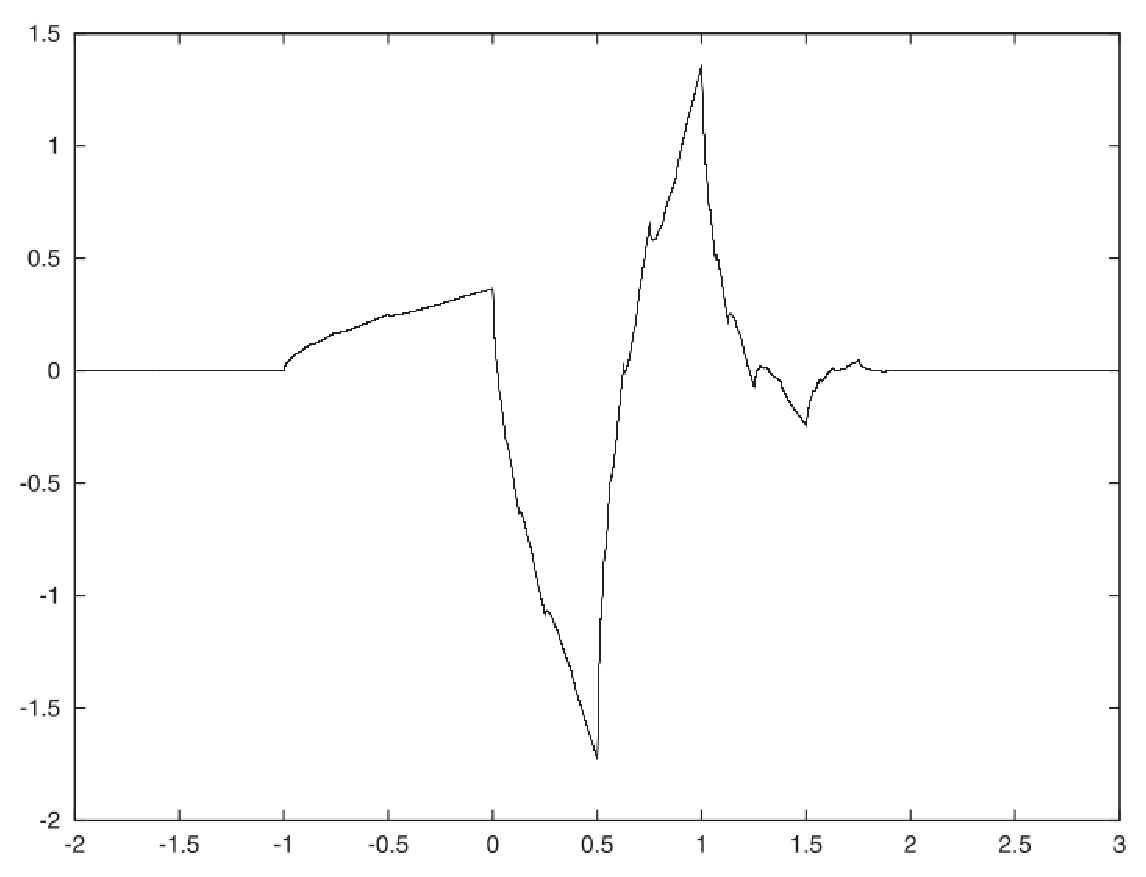
\includegraphics[width=\textwidth]{Figures/dauberchiesWave}
   \end{subfigure}
   \label{fig:wavelets}
   \caption{Dauberchies wavelet (b) and the respective scaling function (a).}
\end{figure}
which already cannot be written in a closed form.
Both wavelets mentioned above are not smooth functions but still posess good properties for practical applications.
Further it is important to note that the explicit evaluation of the functions is not needed for most applications but one rather handles with the coefficients $h_k$ instead.
More smooth wavelet can be obtained at the expense of a non-compact support but they usually decay fast and hence still can be considered as being localised.
%Thereby, a hierarchical set of orthogonal functions is used that describe each features of a given size, making this method suitable for compression, analysis similar to the Fourier method and solving PDEs.\\

Besides their broad use in data compression and analysis, they provide a good basis to solve partial differential equations and are found to have similar numerical properties to FEM \textcolor{green}{sources}\cite{FdFeWavelet}.


\chapter{Finite Element Methods}
\label{ch:fem}
As a conclusion of the previous chapter one can see that the number of methods that are currently available to describe a free electron function in presence of an intricate electrostatic background potential is not that large.
In this work the method of choise to model the free electron function is the FEM which had been applied to quantum mechanical problems already by several authors \cite{fem_hydro, vib_fem, fe_hf, fe_dft1}, however, to the best of my knowledge, only to bound state problems so far.
A brief review about these works is given in section \ref{ch:feQM}.
Besides its large flexibility and computational efficiency pointed out in section \ref{ch:introFEM} already, the large amount of available libraries for FEM \cite{libmesh,dealII,freefem, hermes,oofem} is another advantage of practical importance due to the complexity of the generation of a suitable mesh, assembling of matrices and solution of matrix equations.

In the following chapter the integration of the matrix elements (section \ref{ch:feInt}) and set up of the mesh (section \ref{ch:feAss}) will be described.
Thereby the focus is put on the application to the one-particle SE that is to be solved with molecular electrostatic potential.
Since the interest thereby is on free particle solutions, the spectrum is expected to be very dense and the wave function to be delocalised, requirering for well-designed boundary conditions.
A discussion of various boundary conditions and asymptotic descriptions available for FEM is described in section \ref{ch:BC}.

\section{Finite Element Calculations in Quantum Chemistry}
\label{ch:feQM}
The FEM is mainly known from engineering disciplines where it is used in a broad range of applications such as modelling of fluids \cite{fluid1,fluid2}, heat transfer and flow \cite{heat1, heat2,heat3} or material deformation under mechanical stress \cite{deform1, deform2}.
However, also several different quantum chemical problems have been solved with this method: SE solvers for small systems such as light atoms \cite{fem_hydro,fem_He,fem_He1, fem_h1, LiGS_fem} or diatomics \cite{fem_H_refine}, vibrational model systems \cite{vib_fem} and solid state problems \cite{fem_crystal, fem_crystal1}.
Moreover, even Hartree-Fock \cite{fe_hf} and DFT calculations on systems up to the size of benzene \cite{fe_dft1, fe_dft2, fe_dft3} have been performed, yielding results comparable to those obtained by the usual linear combination of atomic orbitals (LCAO) approach.

The above-mentioned publications have shown that the FEM is able to obtain reasonable results for molecular systems where the errors were comparable to those obtained with standard quantum-chemistry schemes even though their computational costs are higher.
This suggests that the FEM is a good tool for computations in the field of quantum chemistry for going beyond the capabilities of the established schemes such as the description of unbound states.

%\section{From Weak Form to a Matrix Equation}
\section{Integration of Matrix Elements and Formulations of the Equation System}
\label{ch:feInt}
In section \ref{ch:introFEM} the basics of the FEM were described and the generalised eigen system shown in equation (\ref{eq:SEmat}) to solve the SE was derived.
Here this is taken as starting point and a closer look at the computation of the matrix elements as well as solving strategies for the large sparse generalised eigen problems are taken.

The generalised eigenproblem as given in equation (\ref{eq:SEmat}) consists of three matrices.
Since the ansatz functions $\varphi_i(\vec{r})$ have only a small support, most of the matrix elements are zero. 
However, in two and three dimensions no distinct band structure is achievable and the matrices are irreducible.
Thereby matrix elements are zero when the elements involved are not neighboured.
The computation of the non-zero matrix elements involve an integration as \textit{e.g.} the overlap integral $\mat{M}_{i,j}=\int d \vec{r} \varphi_i(\vec{r}) \varphi_j(\vec{r})$ of ansatz functions,.
Since these functions are the same for all elements, the evaluation of these integrals can be done via a lookup-table or an efficient numerical integration scheme whose required order is well-known and need only be multiplied by the Jacobian of the respective elements involved.
The matrix elements $\mat{A}_{i,j}=\int d \vec{r} \left(\nabla \varphi_i(\vec{r})\right)\left(\nabla \varphi_j(\vec{r})\right)$ consist similar to those of $\mat{M}$ of overlap integrals of known functions.
The only matrix containing system-specific information is the potential $\mat{V}_{i,j}=\int d \vec{r} \varphi_i(\vec{r}) V(\vec{r}) \varphi_j(\vec{r})$ which requires numerical integration by which $V(\vec{r})$ is approximated as a spline of given order.

After assembling the matrices the eigenpair $(e_i, \vec{c}_i)$ of the system
\begin{equation} \label{eq:SEmat2}
\left(\frac 12 \mat{A}+\mat{V}\right)\vec{c}_i = e_i \mat{M}\vec{c}_i
\end{equation}
need to be found where $e_i$ should be closest to the analytic value of the kinetic energy of the photoelectron.
Since matrix eigenvalue equations with several thousands of dimensions occur in many fields, numerous schemes have been developed to solve them efficiently \cite{davidson,arnoldi, gpusolver,krylov}, a selection of them is described in section \ref{ch:ghep}.
Despite the numerical complexity due to the high dimensionality of this problem (several thousands of ansatz functions) the second problem is due to the fact that the eigenenergies $e_i$ are expected to be close to each other since the corresponding analytical problem has a continuous spectrum in this range.
It is well known in numerics that this leads to instabilities especially for the eigen vectors, making a regularisation of the problem (described in section \ref{ch:regular}) indispensable.

\section{Element Types and Mesh Types}
\label{ch:feAss}
Among the FEM formulations several `flavours' were designed for different purposes.
Given a certain equation to be solved in FEM there are in general two ways systematic ways to increase the accuracy.
One way is to increase the number of elements witch is referred to as the $h$-FEM approach \cite{dreyer,}.
The refinement of the mesh is in principle always possible but technically demanding since it is not known in which regions of a mesh are too coarse in general \cite{dreyer}.
To overcome this some FEM implementations, such as that of \prog{Libmesh} \cite{libmesh} which is used here, provide an adaptive mesh refinement scheme iteratively refining the mesh using local error estimations \cite{libmesh}.
But theses schemes are numerically demanding and hence can be only applied to benchmark systems.

The second strategy is called $p$-FEM. 
In the $p$-FEM scheme the order $p$ of the test functions in increased, resulting in smother and more flexible solutions.
This scheme requires a large set of functions to be implemented but is known to yield good results if the function is smooth \textcolor{green}{source}.
While standard FEM usually have only $p=1,2$, there are certain special-purpose schemes that go beyond this.
The setup of the mesh is, as mentioned above already, critical to the quality of the solution and hence of special importance.
Moreover, it is technically non trivial to set up a close packing of volume elements with the desired properties in a systematic way.
There are different element types available, each with their techniques for set up.
Although in principle any element shape can be chosen, in three dimensions only tetrahedral (simplex), prism- and pyramid-shaped as well as hexahedral elements commonly are used.
By choosing the element shape and the polynomial order, also the type of ansatz functions is defined.
%When using hexahedral elements the ansatz functions usually are of the type $\varphi(\vec{r})=x^ky^lz^m$ where $p=k+l+m$ is the element order.

When considering meshes to describe molecular properties it is clear that the element size should be smaller in the vicinity of the nuclei while it may be broader at larger distances.
One way to create a hexahedral mesh with local refinement is to start with a coarse uniform lattice and subdivide the hexahedra where necessary as shown in Figure \ref{fig:HexBenz} for a benzene molecule.
Another way is to setup small regular cubic grids around the nuclei and expand them radially in boxes of growing size as shown in Figure \ref{fig:HexDia}.
These brick-shaped elements however have the disadvantages that the regular cube-like structures therein are not well-suited for atoms and molecules that rely rather on spherical shapes.
Further hexahedral elements are known to give less accurate solutions than tetrahedra which are commonly used nowadays \textcolor{green}{cite}.

%\begin{wrapfigure}{r}{\textwidth}
%\includegraphics[width=\textwidth]{Figures/Elements3d-crop.pdf}
%\caption{The different Shapes of 3D elements.}
%\end{wrapfigure}
Another approach used by Lehtovaara \textit{et al.} \cite{fe_dft2} is to put layers of polyhedra around the atoms with increasing number of points and radii.
Thereby the overlapping regions of these spheres are removed by deleting elements that are closer to another atom.
\begin{figure}
   \begin{subfigure}{0.24\textwidth}
   \includegraphics[width=0.95\textwidth]{Figures/QuadMeshBenzene}
   \caption{}
   \label{fig:HexBenz}
  \end{subfigure}
  \begin{subfigure}{0.24\textwidth}
   \includegraphics[width=0.95\textwidth]{Figures/QuadDiatomic}
   \caption{}
   \label{fig:HexDia}
  \end{subfigure}
  \begin{subfigure}{0.24\textwidth}
   \includegraphics[width=.95\textwidth]{Figures/PolyBenzene}
   \caption{}
   \label{fig:PolyBenz}
  \end{subfigure}
  \begin{subfigure}{0.24\textwidth}
   \includegraphics[width=.95\textwidth]{Figures/AdaptiveEthylene}
   \caption{}
   \label{fig:AdapEthyl}
  \end{subfigure}
  \caption{2D cuts through 3D meshes for molecular systems obtained with different schemes for local refinement:
    (a) hexahedral elements adapted for the benzene molecules \cite{fe_dft1}
    (b) hexahedral mesh for a diatomic \cite{fe_hf}
    (c) Polyhedral mesh for a benzene geometry \cite{fe_dft2}
    (d) Adaptive refined tetrahedral Mesh for ethylene. \cite{fe_hf}
    }
\end{figure}
The mesh obtained with this procedure for a benzene molecule \cite{fe_dft1} is shown in Figure \ref{fig:PolyBenz}.

When restricting oneself to tetrahedral elements, other design principles are possible: Since they are simplexes in three dimensions, they can be designed from general grids using \textit{e.g.} Voronoi \cite{voronoi} or Delaunay \cite{delaunay} tessellations (the latter is described in section \ref{app:delaunay} in appendix) from a set of points with the required properties.
Son and Chu \cite{Son_Chu, Son_Chu0} constructed sets of points resembling molecular geometries by inserting $N$ spherical grids with different radii $r_i$ around the atoms and cutting off the overlapping regions.
Thereby the respective radii are chosen as
\begin{equation}
r_i=\frac{il}{N-i+\frac{lN}{r_\text{max}}} \qquad i=1,\hdots ,N 
\end{equation}
where$r_\text{max}$ is the radius of the largest sphere and $l$ is a parameter smoothly changing between a linear $l\rightarrow \infty$ and a $1/r$-mapping.
As spherical grids they suggested the use of Lebedev-grids \cite{lebedev} and a design of Womersley \cite{Womersley2001,Sloan}.
A more detailed discussion about the choices of grids will be given in section \ref{sec:grid}.
%Choises for angular and radial grid distributions in this scheme are discussed in.% the chapters \ref{app:Sphere} and \ref{app:radius} respectively.

A more entangled method is used by Alizadegan \textit{et al.} \cite{fe_hf}. 
They start with an initial guess for the wave function and create a grid whose distances are inverse proportional to the second gradient of the electron density
\[
d \propto \left[ max\left\{\left|\frac{\partial^2 \rho}{\partial^2 x}\right| ,
                           \left|\frac{\partial^2 \rho}{\partial^2 y}\right| ,
                           \left|\frac{\partial^2 \rho}{\partial^2 z}\right| \right\} \right]^{-1}.
\]
which gives an estimate for the error due to linear approximation within each element.
After solving the eigenvalue equation on this grid, they recompute another mesh on the basis of the new function, iterating this procedure several times.
A cut through a mesh obtained by this procedure is shown in Figure \ref{fig:AdapEthyl}.

\section{Boundary Conditions}
\label{ch:BC}
Boundary conditions have not been addressed in this thesis so far for any of the methods but play an important role for the properties of the solution.
Hence there is a large number of boundary conditions.
The simplest case applicable here are Dirichlet-boundaries, requiring the wave function to vanish at the boundaries of the finite element box.
In the FEM this condition can be applied especially simple by setting the coefficients of the outermost ansatz functions to zero.

Due to the large extend of the free particle, these boundaries however are unphysical if they are not applied at distances that are several times larger than the wavelength.
However, considering a particle with $0.1\,$eV kinetic energy, its wavelength is $~4.4\,$Angstroms and the box would need to have a diameter of several tens of Angstroms which is not feasible any more while kinetic energies in the $m$eV-range would lead to even worse scenarios.

%These considerations make clear that a more advanced boundary condition is needed which has only local influence on the wave function.
%In the following sub chapters, three boundaries that can be applied in FEMs are introduced and discussed.
Besides the numerical restriction to a finite box also mapping schemes can be used as \textit{e.g.} $x=\tan (\frac y2)$ that maps $[-\infty:\infty]$ to $[-\pi:\pi]$ \cite{PSbook}.
However, using such a mapping directly is infeasible since the oscillations of the wave function would become arbitrarily sharp in the mapped range and hence the representation of the FEF would still be poor.

\subsection{Complex Absorbing Potential}
\label{ch:cap}
The complex absorbing potential (CAP) is a method often found in the literature when describing particles with infinite extent\cite{bauch1, bauch2}.
In this scheme, an artificial potential usually of the form
\begin{equation}
   W_\text{CAP}(\vec{r})=\begin{cases} i\nu(\vec{r}-\vec{r}_0)^2 & \vec{r}>\vec{r}_0 \\
                                           0    & \text{else} \end{cases}
\end{equation}
is added where $\vec{r}_0$ is larger than the bound part of the system.
Such a potential damps the wave function by reflecting only a small fraction of the wave back into the region of interest \textcolor{green}{sources}.
However, studies with different shapes of these potentials show that it influences the wave function not only close to the boarders and a proper design of the parameters is....

To minimise the error due to the CAP, the parameter $\eta$ can be chosen such that its dependency on the energy vanishes in first order, \textit{i,e.} $\eta\frac{dE}{d\eta}=0$ \cite{CAPccEOM}.
Moreover, due to non-hermiticity the usual scalar product is not suitable when calculating overlap integrals any more.
Too strong $\eta$ makes reflections, too weak $\eta$ lead to unstable resonances, making them strongly basis-set dependent \cite{CAPfreshlook}

The idea of damping down a function and making sure no reflections are scattered back to the region of interest is common to further approaches as \textit{e.g.} absorbing boundary conditions \cite{Engquist}, perfectly matched layer schemes \cite{pmlBook,pml1, pml2} or certain variable transformations \cite{taoDVR}.

\begin{itemize}
   \item Also read zotero: (In)FEM AbsorbBoundariesVS\_InfFE
\end{itemize}

\subsection{Mode-matching Schemes}
Consider the solution in an inner and outer region as different variables following the equations
\begin{equation}
   \nabla^2\Psi_1 +V(\vec{r})\Psi_1-E\Psi_1=0 \qquad \nabla^2\Psi_2 -E\Psi_2=0 
\end{equation}
whereby the outer function needs to satisfy the Sommerfeld condition $r^\alpha \left(\frac{\partial \Psi_2}{\partial r} - ik \Psi_2  \right)\rightarrow 0$.
These equations are coupled by the conditions
\begin{equation}
\Psi_1=\Psi_2  \qquad \nabla \Psi_1 \vec{n}=\Psi_2 \vec{n}
\end{equation}
to ensure continuity of the solution and the gradient normal to the boundary \cite{AstleyMM}.
Thereby, the asymptotic behaviour of the outer function is ensured by taking ansatz functions that individually fulfil the condition and the boundaries enter the weak formulation since the application of Greens' theorem leads to an extra term.

The mode-matching scheme can be considered as a generalisation of the R-matrix approach in a finite element formulation.

\subsection{The Boundary Element Method}
The boundary element method (BEM) can be used as a self-standing method for solving partial differential equations using the weak formulation \cite{bemDai,bemCostabel}.
In its pure form, the BEM solves the problems using only conditions given at its boundaries that are connected to the volume properties via Greens' theorem, the Gauss-Ostrogradskii (divergence) theorem as well as Stokes theorem \cite{bemBook}.
Even though the BEM procedure suffers strongly from the restriction of being applicable only to linear systems for which a fundamental solution is known as well as the disadvantage of leading to dense, unsymmetric matrix equations \cite{bemCostabel} it has some popularity until these days \cite{bem1,bem2,bem3}.
But its main advantages come into play when being used with the FEM \cite{bem-fem} where the FEM can be used to obtain an accurate solution in the inner region and the boundaries are treated with the BEM.
Considering an unbound domain as, \textit{e.g.} the problem of the outgoing electron, the infinite domain $\Gamma$ can be divided into a finite region $\Gamma_i$ where the atoms electrostatic potential leads to ... and the remaining domain $\Gamma_o$ in which the time-independent SE reduces to the Helmholtz-problem whose fundamental solutions are well-known and thus the BEM is applicable \cite{bemCostabel, bettessBEM}.

\subsection{Infinite Elements}
The infinite element approach was developed in the 1980-ths for acoustical caluculations and is specificly designed for the Helmholtz equation and can be understood as a advancement of the BEM that is speciallised for the Helmholtz equation.
The general idea of the infinite elements is that the solution of the radial Helmholtz equation in spherical symmetry is well-known to be of the form
\begin{equation} \label{eq:infAnsatz}
 \Psi(\vec{r}) = \left(\frac ar +\frac{b}{r^2} + \hdots \right) e^{ikr}
\end{equation}
where $k=|\vec{k}|$ is the absolut value of the momentum of the particle and the prefactors thus correspond to different angular momenta of the outgoing electron.
In the complete limit moreover, any function fulfilling the Sommerfeld radiation condition \cite{sommerfeldCond} can be represented.

To use this asymptotic information, in the infinite element region a layer of elements is set onto the outer surface of the finite element region in which the ansatz functions are of the form (\ref{eq:infAnsatz}).
To fulfill the continuity conditions, the front-face of these elements coincides with the outer face of the respective finite element. while their radial faces have ray-like edges with a common centre in the middle of the finite element region.

Since the first formulation of infinite elements, several different schemes were developed with increasing convergence characteristics.
For brevity here only the wave-envelop formulation or Astley-Leis elements will be presented.
An overwiev about different formulations is given in the references \cite{dreyer} and \cite{Astley}.
The main break-through of them is not to use the Galerkin-scheme where the ansatz- and test-functions come from the same space but to chose them of different structure.
While the ansatz functions are of the form
\begin{equation}
 \Psi(\vec{r}) = \varphi(\vec{r}) e^{ik \mu(r)},
\end{equation}
the test functions are of the shape
\begin{equation}
 \Phi(\vec{r}) = D(r)\varphi(\vec{r}) e^{-ik\mu(r)}
\end{equation}
where in three dimensions $D(r)=\frac{1}{r^2}$ \cite{astley2}.
With this choise of respective ansatz functions the Hamiltonian (\ref{eq:FEMmatrix}) is not symmetric anymore but still hermitian.

The functions $\varphi(\vec{r})$ are furthermore chosen to follow the product ansatz $\varphi(\vec{r})=f(r)\varphi_2(\vec{r})$ where $\varphi_2(\vec{r})$ is an ansatz-function of a two-dimensional finite element corresponding to the inner face and  for $f(r)$ Jacobi-polynomial turned out te be most stable \cite{dreyer_improved}.

This choise of ansatz functions has the advantage that the oscillating terms do not enter the matrix elements and due to the factor $D(r)$ the matrix elements are finite even though $\Psi(\vec{r})$ is not square-integrable.
Even though the oscillating term $e^{ikr}$ cancels out, the Hamiltonian is energy dependent and thus the generalised eigenvalue problem (\ref{eq:SEmat}) formulated in chapter \ref{ch:introFEM} changes to
\begin{equation} \label{eq:SEinf}
\mat{A}\vec{c} +ik \mat{B}\vec{c}- k^2 \mat{C}\vec{c} =0 
\end{equation}
with
\begin{align} \label{eq:InFEMmatrix}
\mat{A}_{i,j}& =\int \left(V(\vec{r}) D(r) \varphi_i(\vec{r}) \varphi_j(\vec{r}) 
                 -\frac 12 D'(r) \varphi_i(\vec{r})\varphi'_j(\vec{r})
                 +\frac 12 D(r) \varphi'_i(\vec{r})\varphi'_j(\vec{r}) \right) d\vec{r}\\
\mat{B}_{i,j}&=\frac 12 \int\left( -\mu'(r)D' \varphi_i(\vec{r})\varphi_j(\vec{r})
                + D(r) (\varphi'_i(\vec{r})\varphi_j(\vec{r}) -\varphi_i(\vec{r})\varphi'_j(\vec{r})) \right) d\vec{r} \\
\mat{C}_{i,j}&= \frac 12 \int\left( (D(r) \mu'(r) \mu'(r) + 1) D(r) \varphi_i(\vec{r}) \varphi_j(\vec{r})\right) d\vec{r}
\end{align}
where the relation $E=\frac 12 k^2$ is used \cite{dreyer}.

This reformulation though lead to a quadratic eigenvalue problem instead of the generalised eigenvalue problem from before.
However, assuming that the difference between the eigenvalues of (\ref{eq:SEinf}) and the target energy of the outgoing electron is small, the quadratic eigenvalue problem can be approximated by the generalised eigenvalue problem (\ref{eq:SEmat}) by setting $k$ to the respective target momentum in the Hamiltonian.
However, this approximation, which is applied here for simplicity, needs to be verified.

\section{Solving Large Eigenvalue Problems}
In finite element applications such as those being proposed in this work, matrix equations with hundreds up to hundredthousands of dimensions need to be solved.
This requries elaborate strategies, using the sparsity of these matrices.

The focus here is on solving the generalised eigenvalue problem (\ref{eq:SEmat}) and the quadratic problem (\ref{eq:SEinf}) respectively.
However, efficient strategies are only known for regular eigenvalue problems of the form 
\begin{equation} \label{eq:eigenprob}
\mat{A}\vec{x}=\lambda\vec{x}.
\end{equation}
Hence, the more general forms will be rewritten to become (\ref{eq:eigenprob}) as discussed in the subsections \ref{ch:quadEV} and \ref{ch:GenEV} respectively.
Moreover, since the state of interest is a free state, one needs to expect a high density of states for an appropriate mesh. 
This, however, is a well-known problem in numerical methematics since almost degenerate eigenvalues are very sensitive to small perturbations and their respective eigenvectors even more.
Though the subsection \ref{ch:regular} addresses these problems and a way for numerical stabilisation is sketched.

Finally in the subsection \ref{ch:ghep} a few methos are presented showing how a small number of approximate eigenpairs can be obtained in a numerically efficient way from the usual eigenproblem (\ref{eq:eigenprob}).
% general overview: http://www.sciencedirect.com/science/article/pii/S0377042700004131

How is this inversion done numerically?

\subsection{Quadratic Eigenproblem}
\label{ch:quadEV}
--> Probably this chapter is not of interest here since I don't use the respective formulation!?

\subsection{Generalised Eigenproblem}
\label{ch:GenEV}
The most straight-forward way to reformulate the generalised eigenvalue problem
\begin{equation} \label{eq:Gep}
\mat{A}\vec{x}=\lambda\mat{B}\vec{x},
\end{equation}
is te invert the matrix $\mat{B}$, obtaining the regular Eigenproblem $\mat{B}^-1\mat{A}\vec{x}=\lambda\vec{x}$.
This way is possible as long as $\mat{B}$ is invertable and not too large since inversion is a demanding task and the resulting matrix is not sparse anymore \cite{slepcManual}.

To prevent the use of dense matrices, libraries often do not operate with the matrices themselves but rather with a set of vector on which these matrices act \cite{slepcManual}.
The most popular scheme of this kind is the Rayleigh-Ritz projection where the initial problem is approximated on a small subspace $\mathcal{V}_j=span \{\vec{v}_1,\hdots,\vec{v}_j\}$, spanned by appropriate vectors $\vec{v}_i$.

Projecting the original problem (\ref{eq:Gep}) onto this subspace yields the new system $\mat{\Sigma}_j \vec{s}=\theta\mat{\Theta}_j\vec{s}$ where $\mat{\Sigma}_j=\mat{V}_j^T\mat{A}\mat{V}_j$ and $\mat{\Theta}_j=\mat{V}_j^T\mat{B}\mat{V}_j$ respectively which is only of dimensionality $j$.
The matrix $\mat{V}_j$ is unitary with the rows $(\mat{V}_j)_i=\vec{v}_i$.
After solving this dense but small problem, the original eigenvectors can be approximated as $\vec{x}_j=\mat{V}_j\vec{s}_j$ and $\lambda=\theta_j$.
The obtained eigenpair is a good approximation to the actual one as long as the subspace $\mathcal{V}_j$ contains the respective solution or contains a vector which is at least close to it.
A commonly used approach the Krylov subspace.

\subsection{Stabilisation of Eigenproblems}
\label{ch:regular}
Independent of the efficiency and robustness of the eigensolver in use, seeking solutions of the SE for free particles means that eigenpairs are to be found whose energies are, if the numerical parameters are chosen well, very dense or even degenerate.
Unfortunately, dense-lying eigenvalues lead to numerical difficulties; especially the eigenvectors are known to be unreliable in this case.
In practice, this means that the iterative schemes do not converge anymore, requireing a reformulation of the mathematical probelm.

One way to circumvent the instabilities in the original problem (\ref{eq:Gep}) is to reformulate it as a minimisation problem \cite{H2pDeCleva}.
Therefore equation (\ref{eq:SEmat2}) is rewritten as $\left(\frac 12 \mat{A}+\mat{V} - \varepsilon \mat{M}\right)\vec{c}_i = 0$ where $\varepsilon$ is the target energy.
Since this will have most likely no unambiguous solution, one minimises the residuum
\begin{equation}
\text{min}_{||\vec{x}||=1}\left\{\left||\left(\frac 12 \mat{A}+\mat{V}-E\mat{M}\right)\vec{x} \right|| \right\}.
\end{equation}
Using the $L_2$-norm, this is the same as finding the smallest eigenvalue of
\begin{equation}
\left(\frac 12 \mat{A}+\mat{V}-E\mat{M}\right)^\dagger
\left(\frac 12 \mat{A}+\mat{V}-E\mat{M}\right) \vec{x}_i = \theta \vec{x}_i
\end{equation}
where $\theta$ is a measure for the error in energy.
To avoid the costly multiplication of two matrices, one can use  Hermiticity of the matrices and take compute the
square root as
\begin{equation} \label{eq:SEmin}
\left(\frac 12 \mat{A}+\mat{V}-E\mat{M}\right)\vec{c}_i = \lambda \vec{c}_i
\end{equation}
which is a usual eigenvalue problem \cite{H2pDeCleva} and $\lambda$ with smallest absolute value is searched.

Nonetheless, the latter formulation is only an approximation as the comparison of (\ref{eq:Gep}) and (\ref{eq:SEmin}) shows, the latter approximates the mass matrix$\mat{M}$ as unity $\mat{1}$.
Furthermore, equation (\ref{eq:SEmin}) still is expected to have a very dense spectrum and $\lambda$ is an interior eigenvalue so the initial problem is not expected to be solved in this approach.

Instead of the reformulation, here a regularisation of the problem used, applying the spectral transformation shift and invert.
Starting thit the problem: $\mat{A}\vec{x}=\lambda\mat{B}\vec{x}$ where the eigenvalues closest to the target energy $\varepsilon$ are of interest, the spectrum can be shifted to a target energy of $0$ by
\begin{equation}
\left(\mat{A}-\varepsilon\mat{B}\right)\vec{x}=(\lambda-\varepsilon)\mat{B}\vec{x}
\end{equation}
and than inverted to become
\begin{equation}
\vec{x}=(\lambda-\varepsilon)\left(\mat{A}-\varepsilon\mat{B}\right)^{-1}\mat{B}\vec{x}
\end{equation}
which is equivalent to the usual eigenproblem
\begin{equation} \label{eq:stSI}
\left(\mat{A}-\varepsilon\mat{B}\right)^{-1}\mat{B}\vec{x}=\tilde\lambda \vec{x} \qquad \tilde\lambda=\frac{1}{\lambda-\varepsilon}.
\end{equation}
The formulation (\ref{eq:stSI}) has the advantage that the transformed eigenvalues are well-separated and on the extrema of the new spectrum, making the convergence faster and more stable \cite{str-7}.
\begin{itemize}
\item Why do I prefer to use the first formulation?
\item Computing Interior Eigenvalues with Harmonic Extraction --> still good/nice with ST?
\item Purification of Eigenvectors --> Can it help me to do some nice shit?
\end{itemize}

\subsection{Solving Large Eigenproblems}
\label{ch:ghep}
For the computation of eigenpairs large classes of solvers have been developed with various numerical properties.
Besides direct solvers such as the Gau\ss-elimination, many iterative solvers have been developed that are especially well-suited for large but spares problems.
Besides the famous Jacobi- and Gau\ss-Seidel algorithms which converge only in certain cases, also the Davidson method and several Krylov subspace methods are commonly used.

As discussed in the sections \ref{ch:GenEV} and \ref{ch:regular} already, the solution of a generalised eigenvalue problem involves matrix operations which need to be avoided to keep their sparse structure.

As a popular choise for such classes of problems, the Krylov subspace is used.
An $r$-dimensional Krylov subspace is generated by a vector $\vec{x}$ and a matrix $\mat{A}$ and has the form
\begin{equation}
   \mathcal{K}_r(\mat{A},\vec{x})=span\left\{ \vec{x},\mat{A}\vec{x},\mat{A}^2\vec{x},\hdots,\mat{A}^{r-1}\vec{b} \right\}.
\end{equation}
If $\mat{A}$ is sparse, the evaluation of these expressions is only of order $\mathcal{O}(d)$ where $d$ is the dimensionality of $\vec{x}$.
The vectors obtained with large powers of $\mat{A}$ however usually become more and more linearly dependent.
To prevent this, the vectors usually are orthonormalised subsequently.

An important issue in this scheme is a good choise for $\vec{x}$ which crucially determines the speed of convergence.
If a reasonable start-vector is not given, the space $\mathcal{K}_r$ needs to be extended by increasing $r$ iteratively.
The orthogonalisation method being used distinguishes different Krylov subspace methods such as the Arnoldi \cite{str-4} or Lanczos \cite{str-5}.
In the particular implementation, the Krylov-Schur algorithm is used \cite{str-7} which was introduced 2001 \cite{KrSch}.
To keep the dimensionality low, most schemes restart the algorithm after $r$ reached a certain value, starting with a better guess $\vec{x}$.
The efficient restart is another critical issue in this scheme.
In the Krylov-Schur algorithm \cite{KrSch} used here, the restart is conducted implicitly as described in more detail in ref. \cite{str-7}.

%\subsubsection{Inverse iteration and Power methods}
%not suitable for the initial problem, but maybe for the transformed one?
%How well do they work if only an approximate eigenvalue is known?
%
%\subsubsection{Arnoldi, ... Methods}
%
%more description and some explanations on convergence, compared to other methods etc.: http://onlinelibrary.wiley.com/doi/10.1002/gamm.201490008/pdf
% http://www.ams.org/journals/mcom/1981-37-155/S0025-5718-1981-0616364-6/
% GRMES description: http://epubs.siam.org/doi/abs/10.1137/0907058

% alternative: Jacobi-Davidson: http://epubs.siam.org/doi/abs/10.1137/S0036144599363084


%\chapter{Our Procedure}
\chapter{Applied Protocol}
After describing different approaches to compute PESs and pointing out why the Dyson orbital formalism combined with a finite element method used to calculate the photoelectron function is well-suited for our needs, in this chapter now
the protocol as being used to obtain the PESs will be presented.\\
In the first section, the computation of the initial (unionised) and final (ionised) states will be described.
Thereafter, in section \ref{sec:grid} the setup of the finite element system used to compute the free electron function as well as the dipole matrix element will be described.
In the final section, the computation of Dyson orbitals will be sketched and it will be described how to transfer it to the finite element setup.

\section{Bound State Functions}
The formalism as it was described in \ref{ch:do} can be used with any quantum chemical method that is able to calculate ground and excited state wave functions and respective energies.
Since density functional theory (DFT) and its time dependent counterpart TDDFT have shown to be accurate and numerically cheap methods, we use these methods here.

In this work the calculations are done using a locally modified version of the program package \prog{NWChem} \cite{nwchem} where a more verbose output enables the reconstruction of all molecular orbitals and thus the computation of the DOs.

\subsection{Ground State Density}
It is based on the Hohenberg-Kohn theorem \cite{HohenbergKohn} which states that the ground-state electron density determines the potential in the SE uniquely and with this also the wave-function.
Thus, the electron density contains all information about a given system.
Since it does not point to a way how to determine the electron density without knowing the wave-function, usually the Kohn-Sham scheme \cite{KohnSham} is used where the electrons are described non-interacting particles in a respective pseudo-potential that is made such that the electron density of these Kohn-Sham orbitals corresponds to the real electron density.
Since the particles do not interact with each other, the Kohn-Sham orbitals $\Psi_j(\vec{r})$ are solutions to the partial differential equation
\begin{equation}
\left( -\frac 12  \nabla^2 + V_\text{eff}(\vec{r}) \right) \Psi_j(\vec{r})=\epsilon_j \Psi_j(\vec{r})
\end{equation}
where $\epsilon_j$ is the binding energy of the respective electron and the effective potential 
\begin{equation}
V_\text{eff}(\vec{r})=V_\text{ext}(\vec{r})+ \int \frac{\rho(\vec{r}')}{|\vec{r}-\vec{r}'|} d\vec{r}' + V_\text{xc}(\vec{r})
\end{equation}
can be separated into the external potential $V_\text{ext}(\vec{r})$ which consists of the attractive nuclear electrostatic potential.
The second term is the electrostatic interaction of the electrons. 
With these contributions, this formalism is on the level of theory of the Hartree-theory, missing the exchange and correlation.
The respective contributions are approximated by $V_\text{xc}(\vec{r})$ together with the error in kinetic energy to accound for the fact that the single-electron functions of the Kohn-Sham scheme differ from the real electrons and thus have an other kinetic energy as well \cite{Holthausen}.

Assuming that the Kohn-Sham orbitals coincide with the physical orbitals, which is known to be not the case, the exchange potential acts on an orbital $\Psi_i(\vec{r})$ as
\begin{equation}
V_{x;j}(\vec{r})\Psi_i(\vec{r}) =\int \Psi_j^\dagger(\vec{r}')\frac{1}{\left|\vec{r}-\vec{r'}\right|} \Psi_i(\vec{r}') d\vec{r}' \Psi_j(\vec{r})
\end{equation}
and thus is non-local \cite{Holthausen}, the ``exact'' exchange energy thus corresponds the term $E_{x}=\sum_{i<j}\int \Psi_i^\dagger(\vec{r}) V_{x;j}(\vec{r}) \Psi_i(\vec{r}) d\vec{r}$  respectively.
In DFT usually the exchange energy is approximated as a local functional of the density and its derivative, leading to the so-called local density approximation and gradient corrected functionals.
The Becke \cite{blyp} exchange-functional used in this work has the form
\begin{equation} \label{eq:blypXC}
E_x=\frac 32 \left(\frac{3}{4\pi}\right)^\frac 13 \sum_\sigma \int \rho_\sigma(\vec{r})^\frac 43 d^3\vec{r} 
-\beta \sum_\sigma \int \rho(\vec{r})^\frac 43 \frac{x_\sigma(\vec{r})^2}{1+6\beta x_\sigma \text{sinh}^{-1}( x_\sigma (\vec{r}))} d^3\vec{r}
\end{equation}
where $\sigma$ denotes the spin polarisations and $x_\sigma(\vec{r})=\frac{|\nabla \rho_\sigma(\vec{r})|}{\rho_\sigma^\frac 43}$, the first term is corresponds to the local density approximation and the second one is a semi-empirical gradient correction which is constructed such that the asymtotic behaviour of the exchange energy and electron density
\begin{align}
  \lim_{r\rightarrow\infty} E_x^\sigma(\vec{r}) & =-\frac{1}{|\vec{r}|} \\
  \lim_{r\rightarrow\infty} \rho(\vec{r}) & =e^{-a_\sigma |\vec{r}|}
\end{align}
with $a_\sigma$ is a constant related to the ionisation potential of the system under study \cite{blyp}.
The prefactor of the gradient correction, $\beta$, was determined by fitting to several atomic noble-gas systems and is set to be $\beta=0.0042$ in atomic units \cite{blyp}.

Finally, the correlation energy is defined as the difference between the sum of the previously discussed terms and the correct energy.
The correlation potential is defined as the functional derivative of the correlation energy respectively $V_c(\vec{r})=\frac{\partial E_c[\rho]}{\partial\rho(\vec{r})}$.
In the case of the
The LYP-correlation energy functional is based on the Colle-Salvetti formula which estimates the correlation energy in the Hartree-Fock approach and introduces two parameters that are set by fitting to experimental data \cite{lyp}.

\subsection{Excited State Properties}


\subsection{OTRSH-scheme}
One main issue concerned with the DFT-formalism is that the approximate exchange functional decays exponentially instead of $\frac 1r$ and $\frac{1}{r^4}$ for the exchange and correlation terms respectively.
This wrong behaviour affects the obtained wave functions and thus the orbital energies \cite{Bokareva}.

To reduce this error, so-called range-separated hybrid (RSH) functonals are used, in which the DFT-exchange term is used for small interelectronic distances only, while at larger distances, where correlation effects are not that important, the Hartree-Fock excact-exchange is used.
The interchange between the schemes is done by the separation
\begin{equation}
   \frac 1r = \frac{\alpha +\beta erf(\omega r)}{r} +\frac{1-\alpha-\beta erf(\omega r)}{r}
\end{equation}
where $\alpha+\beta=1$ and $\beta$ are parameters to be chosen.
Besides taking the standard parameters, an ab-initio scheme to chose them is the optimally-tuned RSH (OTRSH) scheme where the functional
\begin{equation}\label{eq:J_ao}
   J(\alpha_\text{opt},\omega_\text{opt})=min_{\alpha, \omega} \left\{ |E_N(\alpha,\omega)-E_{N-1}(\alpha,\omega)-\varepsilon_\text{HOMO}| \right\}
\end{equation}
is minimised, making sure that Koopman's theorem is fulfilled \cite{Bokareva}.
Besides similar functionals which account for the electron affinities or ionisation potentials of lower-lying orbitals, the optimisation according to stability or \textcolor{blue}{the most-straight line of partial charges} can be chosen as equivalent ab-initio criteria.
\textcolor{red}{More details on these schemes? Not mention them at all?}

For this optimization procedure the Gaussian package \prog{G09} \cite{g09} is used with the 6-31G(d) \cite{6-31g,6-31gd} basis set and the functional LC-BLYP \cite{lcblyp}. 
The ground state DFT calculation, determination of geometries and the linear-response TDDFT calculations have been conducted with a locally modified version of \prog{NWChem} \cite{nwchem}, employing the basis set def2-tzvp \cite{def2tzvp} without symmetry restrictions.
The Kohn-Sham orbitals (obtained by ground state DFT) and CI-coefficients (obtained by linear-response TDDFT which yields the configuration interaction singles expansion for a number of excited states) as well as the atomic overlap matrix are interfaced to the in-house software \prog{DYSON} \cite{MAgg} that computes the DOs.
The integration of the overlap matrix in eq. (\ref{eq:DO}) finally is perfomed using \prog{ezDyson} \cite{ezDyson}.

\subsection{Computing the Dyson orbital}
The DO is computed in the framework of this thesis with the in-house code \prog{DYSON} \cite{MAgg}.
%Considering a state as linear combination of CI-states is denoted as weak-coupling representation \cite{McCarthy}.

\section{Free electron function}
The FEF is computed with a finite element scheme, using the program \prog{Free Willy} developed in the framework of this thesis.
It is based on the library \prog{Libmesh} \cite{libmesh} which itself uses sevaral libraries for the required linear algebra and the mesh-setup.

\subsection{Setup of the Grid}
\label{sec:grid}
The most crucial part of the FEM is the mesh under usage. 
In the program \prog{FreeWilly} it is obtained from a set of points via Delaunay triangulation (see \ref{app:delaunay} for details) using the library \prog{tetgen} \cite{tetgen}.
The distribution of these points is responsible for the quality of the obtaind solution and depends on many parameters in a non-trivial way.
The dependence is in particular on
\begin{description}
   \item[The molecular geometry] Close to the cores it should be denser, at larger distances a coarser grid is possible.
   \item[The kinetic energy] of the photo electron which gives the maximum distance between two points
   \item[The largest angular momentum of the Dyson orbital] determines the angular momentum of the photoelectron to be resembled.
\end{description}

In the general scheme the generation of the point-distribution follows the suggestion of Son and Chu \cite{Son_Chu}:
The grid is set up of atomar grids, \textit{e.g.} spherical distributions, each centered at atoms where the overlapping regions are cut off.
The radii of these spheres needs to be much larger than the bond lengthes, holes or interatomic gaps in the molecule to (\textit{e.g.} holes in aromatic rings or the space between ligands of larger molecules).
Using this scheme, the grid-parameters are determined by the size of the larges box $r_\text{max}$, number $N$ of spheres used as well as the radial distribution of them and the angular distribution of points on these spheres.
\begin{figure}
   \includegraphics[width=0.5\textwidth]{water1}
   \includegraphics[width=0.5\textwidth]{water2}
   \caption{Example of a mesh for the water-geometry. It consists of $5$ spheres with constant number of points per sphere. The overlapping regions are cut off. Left: cut through the nuclear plane.}
   \label{fig:molmesh}
\end{figure}

For the radial distribution Son and Chu \cite{Son_Chu0} suggested the scheme
\begin{equation}
r_i=\frac{il}{N-i+\frac{lN}{r_\text{max}}} \qquad i=1,\hdots ,N 
\end{equation}
where $l$ is a parameter to chose.
As an alternative distribution, here the formula
\begin{equation}
r_i=\frac{il}{\left( \frac Ni \right)^p \left(\frac{Nl}{r_\text{max}}-1\right) +1} \qquad i=1,\hdots ,N 
\end{equation}
is to be tested where $l$ and $p\geq 1$ are parameters to chose whereby the condition $N<\frac{r_\text{max}}{l}$ should be fulfilled to prevent the singularity.
%Thereby it is important to mention that in this scheme (in contrast to the above one) the (asymptotic for $r\rightarrow \infty$) maximum distance between two spheres is $l$ and hence could be physically chosen to $l\approx \frac \lambda 2$.

While the distribution of spheres follows, at least on a qualitative level, a clear scheme since it should always resemble the local kinetic energy, the distribution on the surface of each sphere is not that clear.
Qualitatively it is preferable to chose a regular grid but this more challenging.
Since the ... grid, which is known from the ... is clearly a bad choise due to its high density close to the poles, in geological applications often so-called geodesic grids are chosen.

\textcolor{red}{
Some explanations are given here:\\ %https://www.maths.unsw.edu.au/about/distributing-points-sphere
- Lebedev-grid -> try to get spherical harmonics with highest L accurate.\\
-If also required: all weights should be equal: spherical t-designs. \\
Leads directly to the question of uniform distribution.-> not directly by algorithms\\
- other approach: close packings \\
- energy minimisation: Consider nodes as interacting particles -> minimise E for some model potential.\\
see} \textcolor{blue}{http://people.maths.ox.ac.uk/beentjes/Essays/QuadratureSphere.pdf}.
\textcolor{green}{
- crude but fast algorithms
Since in finite element theory the sphere neither needs to be really round nor is there any global functional defined on it,
the complicated distributions described above may be not even needed. 
An other approach therefore is to use an algorithm that gives just a more or less uniform distribution.}

Approach used for climate models: so-called geodesic grids: subdivision of polyhedra, projected onto the sphere\cite{geodesic1, geodesic2}, see also
%http://kiwi.atmos.colostate.edu/BUGS/geodesic/
%http://kiwi.atmos.colostate.edu/BUGS/pdf/ZM-grid.pdf
%http://kiwi.atmos.colostate.edu/BUGS/pdf/conservation.pdf
%http://kiwi.atmos.colostate.edu/BUGS/pdf/ccsr.pdf
for further information.

The point sets I took are from here: %http://web.maths.unsw.edu.au/~rsw/Sphere
\cite{womersley,fliegeMaier}.

The above mentioned techniques show the large variety of different approaches and it is not very clear which one will meet our needs best.
Moreover, here the problem is not only two dimensional but the whole sphere (not only its surface) needs to be subdivided. 
Hence, besides the question of a radial density of different spherical surfaces, also the number of points per sphere as function of the radial distance 
needs to be considered.

Whether the approach of subdividing the atomic meshes into radial and angular parts as opposed to another volume tessellation can be questioned and 
may turn out to be inefficient.
Application of Geodesic grid in calculating surface charges: \cite{geodes_charge}, also mentioning Connolly algorithm (refs 26, 29 therein).

The second scheme has a divergence around $Nl=r_\text{max}$. 
It can be shown that the condition $N\leq \frac rl $ is enough here to stabilise it.

\textcolor{yellow}{
If the above described procedures prove to be too inefficient, one could try to implement some WKB-based scheme similar to \cite{impLDVR} but in 3D.
Thereby, the number of points in a given volume element is determined by $N_i=\frac{\alpha_i}{\alpha} N$ where $\alpha=\sum_i \alpha_i $ and
\[ \alpha_i= \int_V dV \sqrt{2\mu (E-V(r))} \]
.This ensures dense points there, where the potential is lowest and a coarse mesh far away; however, a consistent formulation in 3D would need to be invented.
}

To account for the molecular geometry and the general tendency of the photo electron to oscillate stronger in the vicinity of the nuclei, the mesh is built out of spheres, centred at the nuclear positions.
Thereby, a study of Son \cite{Son_Chu0} had shown that it is numerically most efficient when the overlapping regions of these spheres are cut out.
Figure \ref{fig:molmesh} shows an example for the water molecule.\\
For the radial distribution we will use the the function
\[
r_i = \frac{1+x_i}{1-x_i+\frac{2L}{r_{max}}} L \qquad x_i = \frac{2i}{N_r} -1
\]
suggested by Son \textit{et. al.}\cite{Son_Chu0, Son_Chu}.
The parameters $N_r$, $L$ specifying the number of spheres and their distribution; the larger $L$ is, the denser are the spheres close to the centre.\\
The optimal choise of these parameters as well as the angular distribution of points on the spheres is still an open quetion.
Finally, after putting the points together as described above, they are connected to a Delaunay triangulation using \prog{tetgen} \cite{tetgen}. 
Here additional points may be introduced to guarantee well-shaped elements (\texttt{i.e.} no sharp peaks).
\textcolor{red}{
one scheme suggested by Son and Chu \cite{Son_Chu0}:
\[ r_i=\frac{il}{N-i+\frac{lN}{r_\text{max}}} \qquad i=1,\hdots ,N \]
where $l$ is a parameter to chose.
Own scheme:
\[ r_i=\frac{il}{\left( \frac Ni \right)^p \left(\frac{Nl}{r_\text{max}}-1\right) +1} \qquad i=1,\hdots ,N \]
where $l$ and $p\leq 1$ are parameters to chose. Thereby it is important to mention that in this scheme (in contrast to the above one) the (asymptotic for $r\rightarrow \infty$) maximum distance between two spheres is $l$ and hence could be physically chosen to $l\approx \frac \lambda 2$.\\
The second scheme has a divergence around $Nl=r_\text{max}$. 
It can be shown that the condition $N\leq \frac rl $ is enough here to stablilise it. }

Besides the tricky question about this mapping, also the number of points per sphere depending on the radial distance should be considered. 
In \cite{Son_Chu0} this is chosen to be constant without further discussion but of course there are several possible design criteria as well.
Besides a constant number, also a constant spherical density (hence $N\propto r^2$) are possible; However, it might be sensible to follow a similar idea than in the radial mapping: Being fine close to the nuclei and get coarser with increasing distance.
In particular, I followed the design rule of keeping the space between points in radial direction similar to space between points in angular distribution.
Hence, $d_\text{spheric}=\sqrt{\frac{4\pi r_i^2}{N_i}}\approx r_i-r_{i-1}$.
For the above described radial schemes, this results in 
\[
N_i= \frac{4\pi}{ \left(1-\frac{i-1 }{i}\frac{N-i+\frac{lN}{r_\text{max}}}{N-i+1+\frac{lN}{r_\text{max}}}\right)^2 }
\]
for the first scheme and 
\[
N_i= \frac{4\pi}{\left(1-\frac{i-1 }{i}\frac{ (\frac{N}{i})^p \left(\frac{lN}{r_\text{max}}-1\right)+1}{ (\frac{N}{i-1})^p\left( \frac{Nl}{r_\text{max}} -1 \right) +1 } \right)^2 }
\]
for the latter.\\
The respective radii and number of points per sphere are shown in figure \ref{fig:maps}.\\
Special mapping schemes are the constant radial mapping $r_i=a i$ which corresponds to a constant spherical grid density $N_i=4\pi a^2 i^2$ and an exponential map $r_i=q^i r_0$ which would require a constant number of spherical grid points $N_i=\frac{4\pi q^2}{(1-q)^2}$ according to the rule derived above.

\begin{figure}
\includegraphics[width=0.7\textwidth]{Figures/RadialMap}
\caption{the radius and number of points of the spheres as for $N=15$, $r_\text{max}=5$ and $l=2$.}
\label{fig:maps}
\end{figure}

Since some of the spherical schemes described above allow only for certain numbers of points each, here, the best approximation is used respectively.

\subsection{Benchmark}
\textcolor{blue}{
Tested on Lithium with a sphere with $r_\text{max}=2.8$
1:  Using the mapping of Son with a naive approach, setting the number of circles by hand and growing quadratically with the size  ($N_\text{circle}=20$, $l= 2.0$ , $N= 10$)
2: using the Son scheme with N according to above formula
3: using the tm scheme as described above, p=1
4: using the tm scheme as described above, p=2}

\begin{tabular}{|c|c|c|}
\hline
scheme & \#elements & error in energy [a.u.]\\
\hline
1      & 2370      & 0.496220, 0.520199, 0.572279 \\
2      & 2022      & 0.038136, 0.046119, 0.055691 \\
3      & 2166      &-0.003638, 0.027219, 0.050588 \\
4      & 2338      & none converged \\
\hline
\end{tabular}
Thereby, the number of elements were kept as similar as possible.

\subsection{Obtaining ESP}
 - obtained from \prog{NWChem}
 - interpolation of that grid

\section{Obtaining the DOs}
 - from coefficients to values


\chapter{Results and Discussion}
\label{ch:res}
%In the previous chapters, many different methods that can be used to compute PESs numerically are described and in chapter \ref{ch:proced} the method used within this work is described in more detail.
%In this chapter some results are shown and explained.
Since the method developed in this work combines several techniques that have not been used together so far and quantum-mechanical continuum-function are not treated with the infinite elements technique so far, several conceptual questions need to be clarified before computing actual PESs.
In section \ref{ch:BCbench}, infinite elements are compared with Dirichlet BCs and their respective influence on the properties of the wave function is studied. %In section \ref{sec:NumConve} further benchmarking calculations on some numerical parameters are shown.
These calculations are performed using atomic lithium and hydrogen as test system.
Especially the case of hydrogen is of interest here since analytic solutions to compare with are available.
Thereafter, in section \ref{sec:cs}, the energy-dependence of the cross section for the valence transition of lithium as well as several transitions of carbondioxide are studied, comparing several theoretical approaches with experimental data.
Moreover, the PESs of CO$_2$ and benzene as computed with several theoretical approaches are shown.

\section{Comparison of Boundary Conditions}
\label{ch:BCbench}
In section \ref{ch:BC}, several BCs which give rise to different properties for the solution have been briefly overvied.
Detailed studies on absorbing BCs, non-reflecting BCs as well as complex absorbing potentials can be found in literature \cite{babuska,artBC,capComp,absRev,nrBCrev}.
In this work, Dirichlet boundaries and infinite elements are studied in more detail and the properties of the respective results are compared.
Even though the validity of Dirichlet BCs is questionable for unbound problems, they are easy to apply and their physical consequences provide quite straightforward interpretation of the results.
Thus, they provide a good comparison for the study of infinite elements, whose properties are not studied in this context yet.
The infinite elements are the main objective of this work.
Since they provide a reasonable description for outgoing particles, they allow for a small simulation region, even if the wavelength is very large.
Moreover, they have the correct asymptotic behaviour and hence are expected to produce a good representation of continuum solutions.
In section \ref{sec:DBCbench}, systematic tests are made, studying the dependence of the eigenenergies as well as the properties of the wave function on the parameters of the numerical grid used.
Thereafter, in section \ref{sec:iBCbench}, further tests with infinite elements show the influence of these boundary conditions on the solution.
%First, in section \ref{sec:DBCbench} several properties of the grids introduced in section \ref{sec:grid} are studied with Dirichlet boundaries which are particularly easy to set up and understand in their physical consequences provide straightforward interpretation of the results.
%In section \ref{sec:iBCbench}, several properties of the mesh with infinite elements are investigated.
Since it turns out that the solutions obtained with infinite elements are very sensitive to the parameters of mesh and simulation box, this study is performed more extensively.
%For simplicity, the tests shown here are on atomic systems using, unless specified otherwise, an analytic Coulomb potential with charge $1$, corresponding to the ionised hydrogen atom.


\subsection{Dirichlet Boundary Condition}
\label{sec:DBCbench}
Dirichlet boundaries are conceptually the easiest BCs but are known to have a large influence on the solution, especially for continuous functions since they reflect outgoing waves fully.
%\begin{wrapfigure}{l}{0.6\textwidth}
%\includegraphics[width=0.6\textwidth]{Figures/BC/DBCenergies}
%\caption{double-logarithmic plot of the error in energy of the energetically closest solutions in dependence on the radius
%of the sphere. The comparison with $\propto \frac{1}{r^3}$ shows the general behaviour of the error.}
%\label{fig:dbcRad}
%\end{wrapfigure}
\begin{figure}
\includegraphics[width=\textwidth]{Figures/BC/DirichletBC}
\caption{Results obtained with Dirichlet BCs using different box sizes:
a) double-logarithmic plot from the deviation in energy for the solutions closest to the target energy $E_\text{target}=0.566\,$Hartree as a function of the radius of the simulation box;
b) real part of $d$-wave functions obtained with different boxes ($r_\text{max}=3\,$bohr and number of spheres $N=18$, blue line and $r_\text{max}=10\,$bohr and $N=38$ spheres, red line); Coulomb wave (yellow line) is also presented for comparison;
c) and d) show the deviation in energy for box radii of $3\,$ and $10\,$bohr,\ varying the number of spheres (radial grid density, see \eq{eq:tm_map}) in the box;
e) and f) show the partial wave contributions \eq{eq:PartWaveCoeff} having different angular momenta for the the respective solutions with $r_\text{max}=3$ and $N=16$ (left) as well as $r_\text{max}=10$ and $N=38$, respectively.}
\label{fig:dbcRad}
\end{figure}
Moreover, its requirement for the solutions to vanish at the boundaries results in an artificial discretisation of the spectrum similar to that of bound states.
This leads to a banded spectrum, with the energy gap between two states being dependent on the simulation box size.
%Moreover, these boundaries enforce the real and imaginary part of the solution to be identical up to a scaling operations (such as rotations and reflections for spherical systems) which does not hold for continuum waves such as Coulomb waves as can be seen in Figure \ref{fig:RadFun} and plane waves that have a constant phase shift.

%These properties are found in various tests conducted to find reasonable parameters for application to more complex systems.
To understand the general properties of solutions for Dirichlet BC and to formulate requirements to the mesh quality, the method has been first tested on the hydrogen-like system with $\nicefrac{1}{r}$ ESP.
To do so, the radius of the simulation box $r_\text{max}$ and the number of spheres, $N$, see \eq{eq:tm_map} has been varied to get convergent results.
In Figure \ref{fig:dbcRad} a), the deviation in the energy of $15$ solutions is shown for different $r_\text{max}$ (see \eq{eq:tm_map}), the number of spheres is kept constant at $N=20$.
The comparison with the red line that represents a $\nicefrac{\text{const}}{r^3}$ dependence, shows that the error is inverse proportional to the volume of the box which is a well-known result for particles in a box with infinite potential walls. 
The number of spheres is kept constant at $N=20$.
The influence of radial grid density on the energies is shown in the panels c) and d) of Figure \ref{fig:dbcRad} where the number of spheres is varied for two different box-sizes, $r_\text{max}=3$ and $r_\text{max}=10\,$bohr, respectively.
In these figures several branches of solutions can be seen that correspond to different angular momenta.
For smaller radii ($r_\text{max}=3\,$bohr, panel c)), these branches are well-separated but become closer and interfere with each other at larger radii ($r_\text{max}=10\,$bohr, panel d)).
Following the expectations, the energies of the respective branches decay when the number of grid points.
At $N=18$ for $r_\text{max}=3\,$bohr the results converge and do not change much with further increase of $N$.
However, for $r_\text{max}=10\,$bohr the convergence is much slower and cannot be reached for $N<60$.
In principle, the continuum spectrum should have infinite degeneracy containing FEFs corresponding to arbitrary angular momenta and since larger boxes provide higher density of states it may be considered desirable to take as large simulation boxes as possible.
This in general also agrees with the common logic for quantum mechanical calculations.
However, the density of states is not the only important quantity: The PES intensities beinge the main objective in the present work are calculated using the DO.
Due to the aufbau principle, usually the atomic states with quite low angular momentum are populated.
\textit{E.g.} in molecules and atoms consisting of second period elements one can expect only $s$ and $p$ atomic functionals to be populated in the lowest excited electronic states. 
Thus, one can expect that FEFs only up to $l=2$ could contribute to PES intensities if the dipole selection rules hold.
That is why to reproduce reliable intensities, the computational scheme should favour solutions with low angular momentum.

The panels e) and f) of Figure \ref{fig:dbcRad} show the projections of the solutions to the spherical wave functions with respective kinetic energy and different angular momentum, where the partial wave contribution is defined as
\begin{equation} \label{eq:PartWaveCoeff}
\sum_m|\langle \Psi_\text{n} | \Psi_{\vec{k},l,m}^\text{Sph}\rangle |^2.
\end{equation}
Here $|\Psi_{\vec{k},l,m}^\text{Sph}\rangle$ is the spherical wave \eq{eq:spherWave} with angular momentum $l$ and its projection onto the quantisation axis $m$ and $|\Psi_\text{n}\rangle$ denotes the respective numerically obtained solution.
The comparison is done against the spherical waves and not against Coulomb waves, since confluent hypergeometric functions are difficult to converge for larger $r$ and they are much more computationally demanding.

The testcalculations have shown that for the given energy of the photoelectron of $E=0.566\,$ Hartree the obtained solutions have a well-defined angular momentum only for small boxes where the critical radius is in the order of $r_\text{max}=10\,$bohr.
For larger computational domains, the states are mixed and have large contributions from much higher angular momenta and are very sensitive to different parameters such as the number of spheres $N_i$ and the parameters $s$ and $q$ in  \eqs{eq:tm_map} and (\ref{eq:son_map}) respectively.
Moreover, for example the comparison of the Figures \ref{fig:dbcRad} e) and f) shows that solutions with larger boxes tend to have higher angular momenta which is an important argument in favour of smaller boxes since for most atomic systems angular momenta larger than $4$ are not of interest for practical calculations.
This tendencey can be understood when considering the radial SE \cite{Lifschitz}
\begin{equation}
\frac{\partial^2}{\partial r^2} R(r) + \left(2\left(E-V(r)\right) -\frac{l(l+1)}{r^2}\right) R(r)=0
\end{equation}
where $R(r)$ is the radial solution and $E-V(r)$ is identified as kinetic energy.
Thus, given a particular kinetic energy, the radial oscillations are reduced by a larger angular momentum.
This leads to the interpretation that a particle can `distribute' its kinetic energy between the radial (outgoing) and spherical contributions.
In turn, however, needs a wave with large angular momentum more space and thus these solutions are suppressed in smaller computational domains.

In Figure \ref{fig:dbcRad} b), two solutions with $l=2$ along one axis are shown (the fifth one for $r=3$ and the first one for $r=10$ which are shown in \ref{fig:dbcRad} e) and f) as well) for two different box-sizes and compared to the Coulomb wave, being the exact solution for the $-\nicefrac{1}{r}$ potential.
One can see that al both box sizes the radial structure of the wave function can not be reproduced with Dirichlet BC completely, even though the agreement at $r_\text{max}=10\,$bohr is already reasonable.
However, the analytic solution has a node very close to the boundary of the box and thus the agreement will get worse if the maximum radius becomes larger.
This fact is reflected in the energetic difference as well which is in the mE$_\text{h}$-range for the case of $r_\text{max}=10$ whereas the deviation for the smaller box is almost $1\,$Hartree and thus almost twice as high as the target value.
Except for lucky cases where the box-size matches a node of a particular analytic solution, an acceptable deviation in energy of about $10^{-3}\,$Hartree is reached only for box radii of $30\,$bohr or more.
Such simulation setups lead, however, to solutions with very large angular momentum.
Finally, it should be noted that the occurence of high angular momentum solutions is not a problem on its own and should be typical for solutions close to reality.
However, test calculations show that they come out in an unordered way.
Thus, applying some subspace solvers \textit{e.g.} Krylov one, does not guarantee that solutions with low angular momentum will fall in the considered subspace.
This fact does not represent a problem when only energies are accounted for, however, is crucial for PES intensities.

%\subsection{Complex Absorbing Potential}
%Using a CAP as described in section \ref{ch:cap}, two additional degrees of freedom comared to the Dirichlet BCs arise: the strength $\eta$ of the artificial potential (\ref{eq:cap}) and the offset $r_0$ where it starts, the latter has the only restriction to be larger than the radius of the DO.
%In section \ref{ch:cap} it was suggested to chose the parameters such that the respective derivatives of the energy vanish \cite{CAPccEOM,CAPfreshlook}.
%This procedure is, however, only valid if one solution should be taken into account and thus is not directly applicable here.
%Interpreting the real part of the eigenvalues of the eigenproblem (\ref{eq:SEmat}) as the energy of the respective state, the influence of the CAP on the density of states varies strongly when changing other parameters.

\subsection{Infinite Elements}
\label{sec:iBCbench}
The method making use of infinite elements has more different parameters which can be crucial for the stability of the solution than the Dirichlet BC.
Investigations of these dependences is the subject of the present section.
As described earlier, using the infinite element approach, the SE becomes a quadratic eigenvalue problem due to the oscillating contributions in the basis functions \eq{eq:infAnsatz}.
To reduce the computational costs, in this work the frequency of these oscillations is fixed to correspond to a target energy $k=\sqrt{2E_\text{target}}$.
With this the Hamiltonian depends on the target energy and the solutions obtained are with increasing energetical deviation, less consistent.
However, the obtained solutions with a reasonable error in energy are FEF that are adapted to the real ESP that is large in the finite region and show a consistent asymptotic behaviour.
%In the first part of this section, several of the testcalculations shown above for Dirichlet BCs are 

\begin{figure}%{R}{0.5\textwidth}
\begin{subfigure}{0.53\textwidth}
   \includegraphics[width=\textwidth]{Figures/BC/plane_fin}
   \caption{2D-cut through a FEF obtained with infinite elements using a spherical finite element region indicated by the red circle with a radius of $r=6\,$bohr and $N=11$ spheres for a target energy of $E_\text{target}=2.12\,$Hartree.}
   \label{fig:cutInfa}
\end{subfigure}
\begin{subfigure}{0.47\textwidth}
   \includegraphics[width=\textwidth]{Figures/RBF/p_wave}
   \includegraphics[width=\textwidth]{Figures/RBF/P-Wave}
   \caption{2D-cut through a FEF obtained with angular momentum $l=1$ (upper panel) and the respective analytic Coulomb wave (lower panel) for comparison.
   Box-parameters of the numerical setup: $r_\text{max}=12.39$, $N=18$, radial scheme: tm \eq{eq:tm_map}, $s=2.5$, $q=1.2$, $E_\text{target}=0.133\,$Hartree.}
   \label{fig:cutInfb}
\end{subfigure}
%\caption{Solutions obtained with different parameters }
\label{fig:cutInf}
\end{figure}
In Figure \ref{fig:cutInf}, the 2D-cut of typical solutions obtained with infinite elements for the hydrogen atom are shown.
The red circle in Figure \ref{fig:cutInfb} indicates the region of finite elements.
These graphs illustrate the the asymtotic behaviour of the regular oscillations of an outgoing wave with correct wavelength.
Moreover, the comparison of the numerically obtained results (upper panel in Figure \ref{fig:cutInfb}) with the respective Coulomb wave (lower panel of Figure \ref{fig:cutInfb}) shows a good agreement.
However, the angular momentum of the solutions in Figure \ref{fig:cutInfa} and \ref{fig:cutInfb} differs considerably and seems to depend strongly on the parameters of the numerical setup.
Thus, a detailed study of this setup as presented in the following chapters is of primary importance to be able to control the main properties of the solution.

%\subsubsection{Formulation of Infinite Elements}
\subsubsection{Comparison of Formulations}
\label{ch:bmFormul}
Before taking a closer look at the convergence of different parameters, first the formulation of infinite elements to be used later is investigated.
To avoid the appearance of infinite integrals and respective surface integrations in the integration of matrix elements as they appear in the Burnett formulation, an additional damping-term $D(r)=\nicefrac{1}{r^{2p}}$ with arbitrary $p>0$ can be introduced.
In the standard Astley-Leis formulation, this term is applied to the test function space with $p=1$, leading to a non-hermitian problem.
It is observed, however, that this damping introduces a suppression of low angular momentum-solutions, even though the solution space remains unchanged.
Since especially the low angular momenta are crucial in this work and to avoid the appearance of complex energies, here the influence of the power $p$ in the damping-term is studied and the symmetrised and non-symmetrised formulations are compared.
%Moreover, to study the influence of the damping function in the Astley-Leis formulation (\ref{eq:ALelem}) in more detail, also a test function space similar to eq. (\ref{eq:ALelem}) but using the squared damping function $D(r)^2$ instead of $D(r)$.

The 50 solutions whose energy is closest to the target value of $0.5675\,$E$_\text{h}$ obtained with the original Astley-Leis formulations with the damping function taken to the powers $p=1$ and $p=2$ as well as the symmetrised formulation (\ref{eq:ALsymm}) suggested in this thesis with powers $p<0.5$ are shown in Figure \ref{fig:IFEMform_spect}.
%For the unsymmetric formulations only the real part is shown which is assigned to the physical energy of the respective state.
For the solutions obtained with the unsymmetric formulation, only the real part is presented in Figure \ref{fig:IFEMform_spect} which is assigned to the physical energy of the respective state.
The eigenenergy of a continuum state determines the frequency of its oscillations if it is a real number.
Inserting a complex number in the oscillating function, its imaginary part leads to a damping of the solution and, using a time-dependent description, to a decaying norm of the wave-function.
\begin{figure}[h]
\includegraphics[width=\textwidth]{Figures/IFem_form_spectra}
\caption{The first 50 eigenvalues obtained with the original Astley-Leis formulation (imaginary part not shown) and with the symmetrised form \eq{eq:ALsymm}.
The colorbar denotes the power $p$ of the damping factor $D(r)$ for the symmetric formulation.}
\label{fig:IFEMform_spect}
\end{figure}
Due to this behaviour, complex eigenvalues are interpreted as the energy and lifetime of the respective state.
However, the damping term $D(r)$ that introduces the imaginary part of the eigenvalue is artificial in the case of infinite elements, this lifetime has no physical meaning 
The results presented in Figure \ref{fig:IFEMform_spect} show clearly that the obtained density of states decreases with the power $p$ and converges for $p\approx \frac 18$ for the given parameters (the radial mapping scheme \eq{eq:tm_map} is used with $N=25$, $q=0.5$, $s=2.5$ and $r_\text{max}=7\,$bohr.).
The strong dependence of the obtained spectrum on the power of the damping function indicate that a reasonable asymptotic description is crucial for the properties of the wave function.
Another important conclusion of the , even for small powers $p\approx 10^{-4}$, no numerical instabilities are observed, indicating that the matrix elements are still well-defined.
%The observations made on the convergence-properties using the spectrum in Figure \ref{fig:IFEMform_spect} are supported by the projections of the solutions on spherical waves of which some are shown in Figure \ref{fig:IFEMform_project}.
%
%The dependence of the obtained spectrum of the Hamiltonian on the power of the damping function shows that, at least for FEFs, the asymptotic behaviour is crucial for the properties of the wave function. 
%The dependence converges for $p=1/8$, see also Figure \ref{fig:powerSpect} in supplement.

The fast convergence of the solutions with respect to the power $p$ can be seen also when studying the character of the obtained solutions in terms of the partial wave contribution \eq{eq:PartWaveCoeff}.
In the Figure \ref{fig:IFEMform_project}, the partial wave contribution of $30$ solutions is shown for the original, unsymmetric, Astley-Leis formulation (left panel) and the symmetrised form with different damping powers $p=0.5$ (centre) and $p=10^{-4}$ (right).
The comparison of the solutions obtained with the unsymmetric and the converged ($p=10^{-4}$) symmetric formulation shows that these states have contributions of different angular momenta in a similar ratio.
Especially for low angular momenta, the symmetric formulation seems to be beneficial if the damping is small enough.
\begin{figure}[h]
\includegraphics[width=\textwidth]{Figures/Ifem_forms}
\caption{Decomposition of the first $30$ solutions into spherical waves with angular momenta up to $l=7$.
Left: Astley-Leis-formulation ($p=1$), centre: symmetrised form ($p=0.5$) right: symmetrised form ($p=10^{-4}$).}
\label{fig:IFEMform_project}
\end{figure}
However, for larger powers $p$ such as $p=0.5$ as given in the centre panel of Figure \ref{fig:IFEMform_project}, the contributions with angular momentum $l<2$ are completely suppresed.
Hence, even if less contributions of different angular momenta are observed in case of $p=0.5$, the results obtained with this formulation should not be taken into account.
This fact can be understood by considering that the case $p=0.5$ corresponds to an additional factor of $\nicefrac{1}{r}$ in the multipole expansion and thus $s$-waves should be always suppressed in this case.
Chosing the power small enough, however, leads to vanishing influence on the character of the solution.
However, as shown in the Figure \ref{fig:IFEMform_project}, the nature of the states obtained is in all cases strongly mixed in the quantum number $l$ with significant contributions even for $l>7$ which corresponds to the white spaces in Figure \ref{fig:IFEMform_project}.
However, the relative contributions of the angular momenta critically depends on the power $p$, making a reasonable choice of this parameter important.
%Further it is expected that the convergence of $p$ depends on further parameters such as the box-size and kinetic energy of the photoelectron which is, however, not studied here in more detail.
In the rest of this work, the power of the damping function $D(r)$ is chosen to be $p=0.0001$.
This value is by far converged and thus is considered to be reasonable also for other systems.

The mixing od different angular momenta should be, at least in the atomic case, avoidable since the angular momentum operator $\hat{L}$ has the same set of eigensystems as the Hamiltonian.
However, for atomic cases as studied here, the eigenstates should be eigenfunctions of the angular momentum operator $\hat{L}$.
In the analytic case of the hydrogen atom, all angular momenta are degenerate and thus belong to an invariant subspace.
However, for FEFs the discussion of degeneracy is, ambiguous since the solutions are infinitely degenerate at any given energy and thus for any system with radial symmetry a degeneracy of $l$ is present.
It should be noted that this discussion is not true for Dirichlet BC, since these boundaries can be considered as an infinitely high potential well and thus, even in analytic case, the spectrum is discrete and the solutions not degenerate in angular momentum.
%\begin{figure}
%\includegraphics[width=\textwidth]{Figures/RadWave_p0_001.pdf}
%\caption{The eigenenergies for different box sizes (coloured dots in the upper panel) where the box size is denoted by the colour in atomic units.
%The lower panel shows the decomposition of the solutions into spherical waves for three box sizes, marked by a star in the colour bar respectively.}
%\label{fig:RadWaves}
%\end{figure}

Keeping this discussion in mind, the mixing of different angular momenta is caused by the numerical scheme.
The discreteness of the basis in use lifts the infinite degeneracy and, due to numerical irregularities such as the stepwise linear character of the finite element scheme, the high symmetry is disturbed.
It can be shown that the influence of these numerical disturbances on the eigenstates becomes larger, the denser the spectrum is.
Considering the eigensystem $\mat{A}\vec{u}=\lambda\vec{u}$ to be solved, any disturbance can be considered as caused by a matrix $\mat{E}$ that is added to the matrix $\mat{A}$.
Assuming that $\mat{A}$ is a hermitian matrix, the eigenvector $\vec{u}_i$ is changed according to \cite{saad, wilkinson}
\begin{equation}\label{eq:ErrVect}
\delta \vec{u}_i=\sum_{j\neq i} \frac{\vec{u}_j^\dagger\mat{E}\vec{u}_i}{\lambda_i-\lambda_j} \vec{u}_j
\end{equation}
where $\lambda_i$ is the eigenvector corresponding to $\vec{u}_i$.
Accordingly, \eq{eq:ErrVect} represents a direct connection of a dense spectrum and the strong mixing of angular momenta.
%From eq. (\ref{eq:ErrVect}) now the coupling of angular momenta and strong dependence on the parameters for a dense spectrum, \textit{i.e.} small $\lambda_i-\lambda_j$ becomes obvious.

%\subsection{Size of Finite Element Region}
\subsubsection{Radius of the Finite Element Region}
\label{ch:bmSize}
%More important than the subspace used numerically is obviously the size of the sphere used for the FEM description.
Similarly to the Dirichlet BCs discussed in section \ref{sec:DBCbench}, the size of the finite element region has a strong influence on the solution obtained with the infinite BC.
A study of the energies of solutions closest to a target value of $E_\text{target}=0.5664\,$Hartree for different box sizes is presented in Figure \ref{fig:InfBoxc} where, except for the boundary conditions, no parameters are changed with respect to Figure \ref{fig:dbcRad} (a).

Comparison of the respective graphs shows that the error is in general smaller when infinite elements are applied which is an indication for the higher accuracy compared to Dirichlet boundary conditons.
Further, the comparison of the obtained solutions with the $\frac{1}{r^3}$-curve in both figures demonstrates that the dependence is much weaker for infinite elements because the solution is not restricted to decay within the range of the finite box.
\begin{figure}[h]
\includegraphics[width=\textwidth]{Figures/BC/BoxsInfEL}
\caption{a)Double-logarithmic plot of the error in energy for different radii of the finite element region.
b)-d) partial wave contribution \eq{eq:PartWaveCoeff} of the $15$ eigenenergies with smallest error;
the box-sizes are: b) $r_\text{max}=4\,$bohr; c) $r_\text{max}=8\,$bohr; d) $r_\text{max}=20\,$bohr and $N=20$ sheres are used in all cases.}
\label{fig:InfBoxs}
\end{figure}
On the other side, the angular momenta of the solutions are in general larger than those occurring with Dirichlet BC for the same box-size.
Moreover, the partial wave contributions (see \eq{eq:PartWaveCoeff}) shown in panels b) -- d) indicate that the angular momenta are much stronger mixed than in the case of Dirichlet BC which.
As discussed above, this is a direct consequence of the higher density of eigenenergies in this scheme.
The white space in the graphs c) and d) corresponds to contributions of angular momenta larger $l>7$ which are not computed here.
Most of the solutions obtained with box-sizes with $r_\text{max}>20\,$bohr, the contributions of angular momenta lower than $l=8$ vanish.
However, the appearance of solutions with significant contibutions of $l=2$ ($d$-wave) in figure \ref{fig:InfBoxs} d) shows that the growing angular momentum with increasing box-size is a general trend but does not hold strictly.

\subsubsection{Density of Spheres}
\label{sec:BenchSphere}
%Increasing the number of spheres has a considerable influence on the energies of FEFs but also changes the angular momenta of the solutions.
The influence of the number of spheres $N$ for a given box is another important parameter whose convergence-properties are important to understand.
A fundamental lower boundary for this is due to the wavelength of the function to be resembled.
However, a quantitative estimation of the convergence with respect to this number is not easy to make in general and depends on many further properties.

Numerical tests on this dependence for a given setup ($r_\text{max}=10\,$bohr and $E_\text{target}=0.5664\,$Hartree) are presented in Figure \ref{fig:InfNum}.
Similar to the behaviour found for Dirichlet BCs earlier in this work, a larger number of spheres leads to larger angular momenta as the comparison of the partial wave contributions in Figure \ref{fig:InfNum} for different numbers of spheres shows.

\begin{figure}[h]
\includegraphics[width=\textwidth]{Figures/BC/NumInfEL}
\caption{The energy and partial wave contributions (\ref{eq:PartWaveCoeff}) for different number of spheres $N$ using infinite elements. The radius is $r_\text{max}=10\,$bohr, respectively.}
\label{fig:InfNum}
\end{figure}
Moreover, the error in energy shown in panel a) of Figure \ref{fig:InfNum} indicates that the shown configurations are far from saturation.
However, since high angular momenta are not desireable, a smaller number of spheres is better suited even though it is not converged.
Thus, the requirements of a low error in energy and high accuracy of the wave function are contrary to the need to have low angular momenta which are needed to obtain reasonable transition dipole moments.

In addition to this, the properties of the solutions presented in Figure \ref{fig:InfNum} change in an unsystematic way when the number of spheres $N$ increased.
As an example for this unsystematic behaviour, the energies of the FEFs obtained with $N=10$ spheres show a much largererror in energy than the solutions obtained with different setup.
The large error, in turn, is also reflected in a weak mixing of angular momenta as the comparison of panel c) with b), d) and f) shows.
%Not only the unsystematic behaviour, the strong dependence of the angular momentum on the number of spheres as such is surprising since, in principle, the radial and angular nodes should be represented with a similar quality.

\subsubsection{Radial Order}
Using the infinite element scheme, a set of additional basis functions is added to the finite element representation having form
\begin{equation} \label{eq:infAnsatzRep}
\Psi(r) = \left(\frac{a_1}{r} +\frac{a_2}{r^2} + \hdots \frac{a_{o}}{r^o} \right) e^{ikr}
\end{equation}
which corresponds to a truncated multipole expansion of order $o$.
As mentioned in section \ref{ch:InfEl}, the term with $o=1$ corresponds to the radial behaviour of an $s$-wave whereas higher radial orders describe the asymptotic behaviour of waves with respectively larger angular momentum.
\begin{figure}[h]
\includegraphics[width=\textwidth]{Figures/BC/OrdInfEL}
\caption{The error in energy for $15$ solutions obtained with a box with radius $r_\text{max}=10\,$bohr and $N=40$ spheres using different orders of the multipole expansion, see eq. (\ref{eq:InfansatzRep}).}
\label{fig:InfOrd}
\end{figure}

Having this in mind, the intuitive solution to the problems with large angular momenta and strong mixing of different contributions might be no restrict it by setting the maximum order $o$ to a respectively low value.
However, the results presented Figure \ref{fig:InfOrd} for different orders $o$ show a more intricate dependence.
The decreasing error in energy can be understood easily since a large amount of additional degrees of freedoms is added to the system.
However, a closer look at the character of the obtained solutions reveals that the angular momentum tends to decrease with larger orders in the multipole expansion \eq{eq:infAnsatzRep}.
The projection of the solutions onto spherical waves presented in Figure \ref{fig:InfOrd} shows that the computed FEFs have a partial wave contribution of about $0.2$ summed over all angular momenta up to 7 when only the first-order terms are taken into account.
However, the FEF with more degrees of freedom show by far larger contributions for the studied angular momenta.

\subsection{Conclusion on Boundary Conditions}
The study of different parameters has revealed several properties of the finite element setup.
An important conclusion of these tests is that a higher density of eigenenergies, which is considered as an indication for a more exact representation of the wave function, in general leads to the appearance of larger angular momenta and to strong coupling of different angular momentum contributions.
This dependence can be easily understood for the size of the computational domain $r_\text{max}$, since wave functions with larger angular momentum have a larger radial extend, but is not that straight forward in the case of number of spheres $N$.

Moreover, it was found that a high density of states usually leads to a stronger mixing of different angular momenta which seems to be a characteristic of this computational scheme.
However, the studies presented here show that a systematic setup of reasonable parameters is non-trivial and needs to  represent a compromise between a dense spectrum and reasonable radial dependence of the wave function on the one side, and low angular momenta as well as well-behaved solution on the other side.

\section{Energy Dependence of the Cross Sections}
\label{sec:cs}
The relative heights of different features in PESs are dependent on the energy of the incoming photons.
This dependence is small if the kinetic energy of the outgoing electron is high, but for low kinetic energies, \textit{i.e.} below $\approx 10\,$eV, the reproduction of the correct energy-dependence is important for a theoretical method to be able to predict the intensities in the PESs reliably.
In the DO formalism, this dependency is accounted for.
In general, the oscillations in the FEF become faster with increasing kinetic energy and thus, the overlap with thed DO, which usually has only few nodes, decreases.
In the limit of very fast oscillations the cross section becomes almost independent of kinetic energy, making the basis for the so-called sudden approximation \cite{saAberg}.
The main influence of this integral is the fact that the oscillations in the FEF become faster with increasing kinetic energy and thus, the overlap with the DO, which usually has only few nodes, decreases.
The slope of the decay with increasing photon energy thus contains information on the spatial extent of the DO.
For a broad and unstructured DO, the oscillations cancel most contributions out, whereas for a strongly localised DO is less sensitive to the wavelength.
%Moreover, a more complicated dependence of the intensity of a peak on kinetic energy including maxima indicates 
Thus, the dependence of the intensity of a peak on the photon energy contains information on the nature of the transition and is studied in a number of experimental and theoretical works for atomic systems as well as small molecules \cite{do_modCoul,LiNaRef1,LiCS,stieltje}.
In this work, the cross section of the valence transition of the lithium atom and the CO$_2$ molecule are studied.

In Figure \ref{fig:Li-CS}, the experimental intensity of the valence ionisation transition of lithium (binding energy of $E_b=0.2067\,$E$_\text{h}$) is shown as a function of the photon energy.
Since the kinetic energy (and thus the wavelength) of the particle spans over a very broad range, the computational setup for the FEF needs to be adapted to the particular kinetic energy of interest and should comprise some oscillations of the FEF in the discrete region.
The studies in section \ref{ch:BCbench} showed that the box-size is very critical to the properties of the solution.
It may not be too small to ensure a reasonable error in energy, but should not be too large to have considerable contributions of solutions with low angular momenta that is crucial for the computation of intensities due to the reasons discussed in section \ref{ch:BCbench}.
\begin{figure}
\includegraphics[width=\textwidth]{Figures/Lithium/CrossSect2}
\caption{a) The photoelectron cross section of the lithium atom as a function of the photon energy obtained by the FEM (Dirichlet BCs (DBC) and infinite elements (Inf)) and the Coulomb wave expansion (Coulomb), compared to experiment \cite{LiCS}.
The intensity is computed as sum over the intensities of $80$ FEFs;
b) The intensities corresponding to individual FEFs are shown.
c) and d) contour plots of the FEFs with the largest intensity contributions with Dirichlet BC (c) and with infinite elements (d), respectively.
Their corresponding peaks are marked in panel b). }
\label{fig:Li-CS}
\end{figure}
To account for this, the box-size was choosen to be $0.8\lambda$ in case of Dirichlet BC and $0.5\lambda$ for infinite elments, where $\lambda=\nicefrac{2\pi}{k}$ is the asymptotic wavelength (\textit{i.e.} reached outside the influence of the Coulomb potential) of the respective target energy.
The box-size smaller than $\lambda$ in case of Dirichlet BCs is too small for a reasonable error in energy but show, since the wavelength is considerably smaller in the presence of a Coulomb potential, still some radial nodes.
For all setups, $N=18$ spheres and the radial mapping scheme \textit{tm}, \eq{eq:tm_map}, with the parameters $q=2.5$ and $s=1.2$ was used, respectively.
For the infinite elements the radial polynomial is truncated after the first order to suppress higher angular momenta.

The intensities obtained with the finite element scheme are presented in two different ways in Figure \ref{fig:Li-CS}.
In the left panel, the $80$ energetically closest intensities are summed up whereas in the right panel the individual intensities are shown.
The theoretical results are scaled to be in good agreement with the experimental data.
For the results obtained with the Dirichlet BCs, the summed intensities (left panel of Figure \ref{fig:Li-CS}) show a systematic but qualitatively wrong behaviour which can be explained by the box which is considerably too small to ensure the correct shape of the wave-function.
However, the intensities of the single transitions (right panel of Figure \ref{fig:Li-CS}) have a different progression.
%Since their energetic position corresponds to their actual kinetic energy, it can be seen that the solutions obtained are in general energetically too low so that no transitions above $0.6\,$E$_\text{h}$ occur.
The qualitative difference between these schemes can be explained by the fact that in the right pannel at lower kinetic energies many transitions contribute with a considerable intensity whereas at higher kintetic energies only few solutions contribute.
Moreover, the transitions can be strongly reordered between the graphs since deviations between the target energy and eigenenergy of up to $0.11\,$Hartree occur.

The results obtained with infinite elements show a less systematic behaviour: Among the hundreds of solutions computed, only three contribute significantly to the cross section.
The scaling factor of the transitions shown in the right panel of Figure \ref{fig:Li-CS} are $0.7$ for the soltions obtained with the Dirichlet BC and $0.4$ for those computed with infinite elements, thus their relative scale is in the same order of magnitude.
These results show that, even for a small computational domain as it is used here, only a poor agreement with the experiment is achievable.
In case of Dirichlet BCs, the bad agreement with the experimental data can be explained by the size of the box which restricts the solution to low angular momenta but introduces a large error in the shape of the wave function and thus influences the dipole matrix elements considerably.
A study with a more reasonable radius of $r_\text{max}=3.5\lambda$ was conducted as well and is shown in Figure \ref{subfig:LiCS}.
However, even though the eigenenergies are denser and the wave function are more flexible, only few transitions with considerable intensity were obtained.
Another important question concerns the normalisation of the wave function.

In the case of infinite elements, too few transitions contributing to the intensity are obtained for an analysis of their kinetic-energy dependence.
However, this shows that even for such a small box, the angular momentum is in general too high to give considerable contributions, at least for $s$-type DOs.

\textcolor{green}{
\begin{itemize}
   \item Explain, why a systematic setup over such a wide range of kinetic energies is not possible for the given scheme. This problem can be seen esp. for DBC comparing left and right of \ref{fig:Li-CS}.\\
    This should be already the main reason for the unsystematic results!?
\end{itemize}
}

\textcolor[rgb]{1,0.7,0}{
   The intensities obtained with the Coulomb wave function are, similar to the results obtained with the FEM and Dirichlet BC, in poor agreement with the experimental data.
   Since the ESP of lithium is very close to that of hydrogen, this is surprising.
   Moreover, the shape makes no sense at all.
}

\textcolor{blue}{
For the computation of the overlap integral, only the finite region is taken into account since outside of it the DO vanishes and thus the outer region would not lead to further contributions.
In this region usually, the wave function is normalised to one which is, especially in the case of Dirichlet boundary conditions, the usual normalisation.
However, if the intensities obtained with different box-sizes are to be compared, two wave functions that coincide in the central region but are computed on differently large regions would result in different intensities.
To account for this, here the wave functions are normalised to the volume, \textit{i.e.}
\begin{equation}
\int_V \left|\Psi_n (\vec{r})\right|^2d\vec{r}=\int d\vec{r}=V
\end{equation}
where $V$ is the volume of the finite element region.}

\textcolor{red}{
For the second testing-system, here first the PES as a whole should be discussed.
\begin{itemize}
   \item assign transitions
   \item The first IP is reproduced well, due to OTRSH-scheme used.
   \item The positions of the other bands are strentched
   \item A considerable part of the features not reproduced, since vibronic progression is not studied here;
   \item SA and DOS are similar (!?) integration changes heights -> improves agreement with experiment.
\end{itemize}
}

For the first two transitions, that correspond to degenerate DOs with $\pi$-character respectively, here also the cross section dependence on the photon energy is studied.
In Figure \ref{fig:CO2CS}, the energy-dependence of the first two transitions shown in Figure \textcolor{red}{that showing the PES} is shown as obtained with various theoretical methods.
\begin{figure}
\includegraphics[width=\textwidth]{Figures/CO2/CrossSect}
\caption{\textcolor{red}{Add labels!} The intensity of the two energetically highest transitions of CO$_2$ as a function of photon energy.}
\label{fig:CO2CS}
\end{figure}
Comparing the results obtained with the multiple scattering method \textcolor{green}{citation} and the Stieltjes imaging approach \cite{stieltje}, a reasonable agreement is achieved.
Both approaches reproduce the main behaviour of the function.
However, for small kinetic energies, both methods do not reproduce the experimental data that well.
The larger problems in case of the $\pi_g$-transition (Figure \ref{fig:CO2CS}) can be explained by the higher binding energy of $...$ and thus lower kinetic energy compared to the $\pi_u$-transition whose cross section is shown in Figure \ref{fig:CO2CS}.

The respective results obtained with the Coulomb wave expansion show also good agreement in case of the $\pi_g$-transition.
In the case of the $\pi_g$-transition, the intensity is highly overestimated for lower photon energies but shows a similar dependence for photon energies larger than about $1.3\,$Hartree.
The good agreement of the results obtained with the approach using a Coulomb wave shows that this approach is more reliable than one might expect, even for highly non-spherical systems such as CO$_2$.
Similar results have been abtained also by Gozem \textit{et.al} who investigated the photoenergy dependence of various transitions of atomic and small molecular systems and showed that the charge $Z$ in the expression for Coulomb waves can be tuned such that an overall good agreemence is achieved \cite{do_modCoul}.

Studying the intensity of these two transitions with the finite element protocol developed here, shows, similar to the results of lithium shown in Figure \ref{fig:Li-CS}, a very unsystematic behaviour.
However, for both transitions studied here, at least a general trend can be extracted which is very similar for both BCs used.
In the Figure \ref{fig:COC2S} a) this trend is in good agreement with the experimental values.
However, the intensities computed for low photon energies in Figure \ref{fig:CO2CS} indicate, that the scheme in use is also not well-suited for the case of low kinetic energies.
It is important to note at this point that the results obtained here have in general a too unsystematic behaviour to draw reliable conclusions from these results.

Despite the problems of finding a setup for which the properties of the solutions can be governed in a reasonable way are addressed above already. \textcolor{blue}{<-reformulate!}
However, in addition to this, another general question arises when using multiple FEFs for determining the intensiy of a transition is that for convergence.
While it is clear that the use of one particular solution for the computation of intensities is in general not a valid scheme, the summation over multiple solutions is only reliable if it converges at a predictible number of states being used.
\begin{figure}
\includegraphics[width=\textwidth]{Figures/CO2/Cronverge}
\caption{Convergence of intensities for the $\pi_g$-transition of CO$_2$.}
\label{fig:cronverge}
\end{figure}
In Figure \ref{fig:croverge}, such a study is shown for the intensities obtained for one of the degenerate $\pi_g$-DOs at different photon energies.
Similar to the studies shown above, here also the radius of the computational domain is adapted to the wavelength.
The cross section here is summed over all states up to the given solution.
The FEF contributing most to the intensities of the studied configurations are shown in the graph to illustrate ????.
As the comparison of the development of the different solution shows, here no convergence is reached.
Instead, the continuum functions with considerable contributions to the transition strength are not systematically distributed.

With this there is no hope anymore. So lets make something different:

Figure \ref{fig:benzPES} shows the PES of benzene obtained with this setup using a grid of height (orthogonal to the molecular plane) of $8\,$\AA\, and a diameter of $12$\AA\, in both directions of the molecular plane with $380$ points in each direction.
\begin{wrapfigure}{L}{0.5\textwidth}
%\begin{figure}
   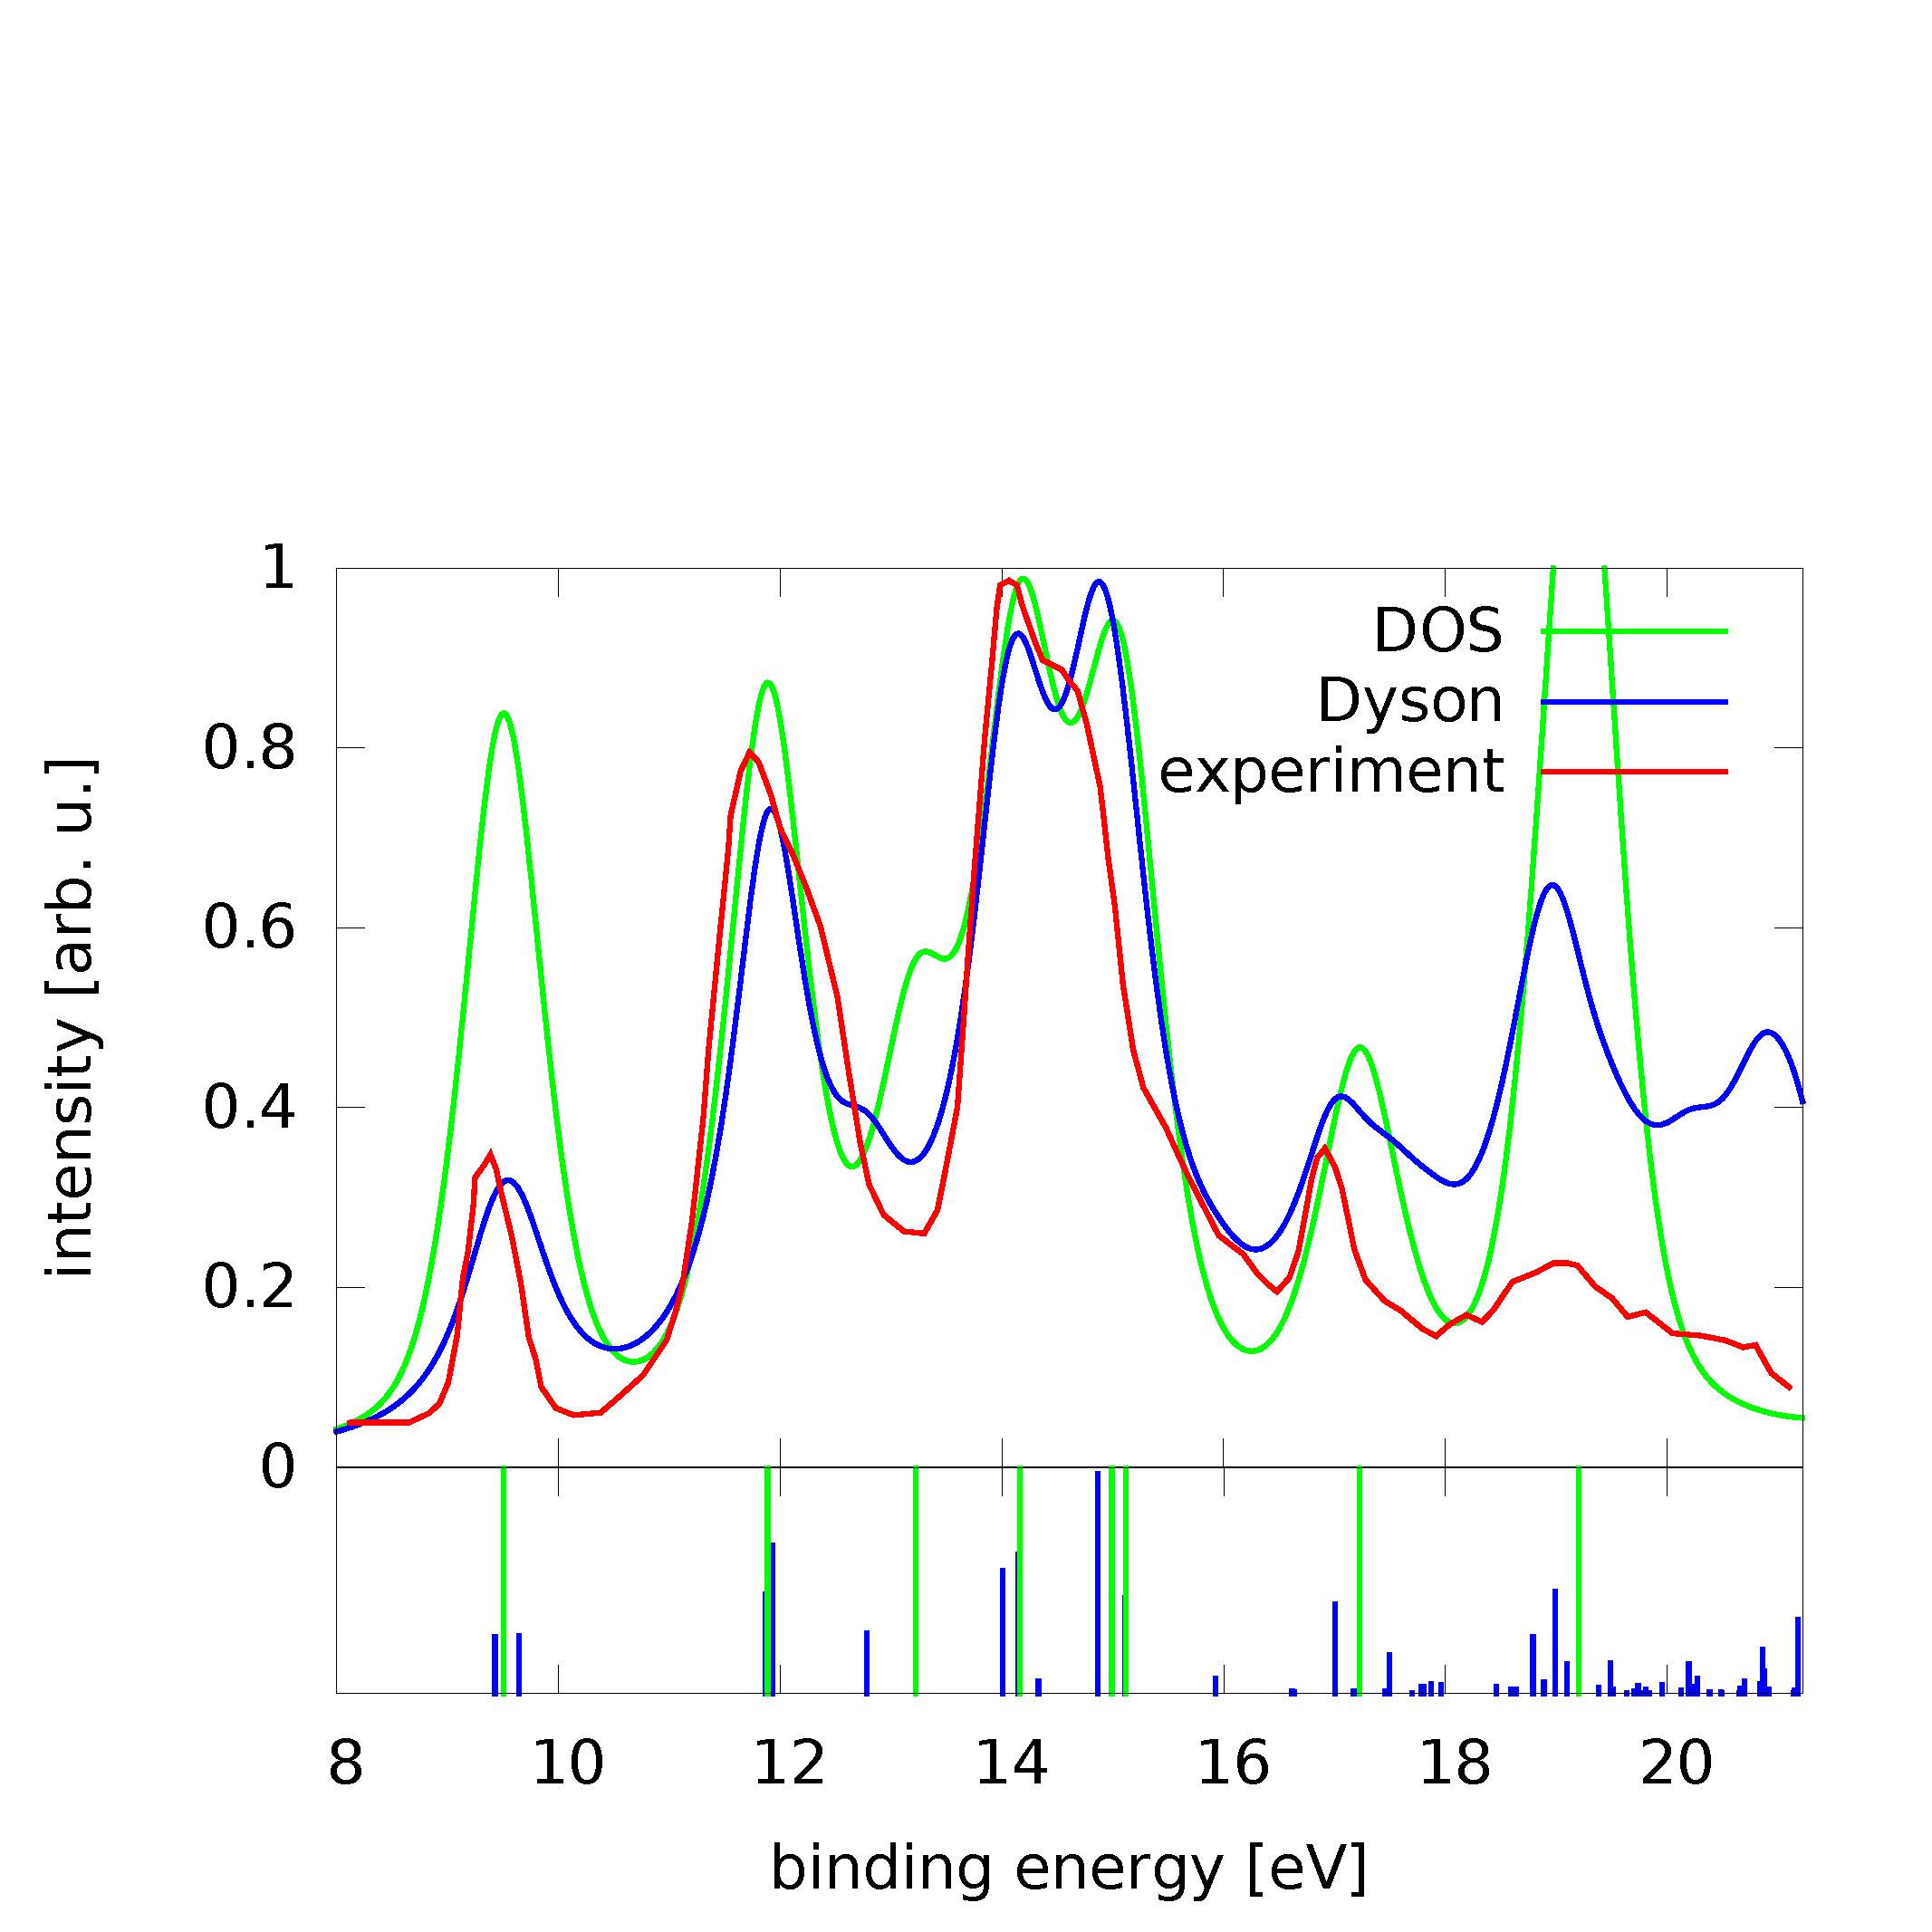
\includegraphics[width=0.5\textwidth]{Figures/Benzene/Benzene}
   \caption{Photoelectron spectra of benzene at different levels of theory.
   In the upper panel the spectra obtained with the Dyson orbital formalism (Dyson) and using the Koopmans' approach (DOS) are compared, the experimental reference is shown in the lower panel \cite{BenzExp}.}
   \label{fig:benzPES}
%\end{figure}
\end{wrapfigure}
The expansion of Coulomb waves includes the terms up to an angular momentum of $l=10$.
The second spectrum shown in 
To indicate the consequences of the OTRSH procedure, in Figure \ref{fig:blypPES} the PES of benzene as predicted with the optimised functional and the B3LYP functional are shown.
For this system, the agreement is good, for other systems the differences are much larger as the example of S$_8$ in the supplement shows.
\begin{figure}
   \includegraphics[width=0.8\textwidth]{Figures/CO2/CO2_spect}
   \caption{}
\end{figure}
\textcolor{red}{
OTRSH is known no be not very good for linear molecules --> is there some reason for this?
}


\chapter{Conclusions and Outlook}
In present work, the theoretical approach to the photoelectron spectra of molecules of arbitrary symmetry is attempted uniting the three essential concepts which can be considered being state-of-the-art by themselves but have not been tried together. In the heart of the method is the electronic structure approach utilizing optimally-tuned range-separated density functional which is obtained in a fully automated self-consistent procedure. With this, the asymptotic behaviour of electron density is corrected, due to the elimination of the self-interaction error, which leads to notable improvement of various molecular properties. By construction, it is particularly suited for predicting valence photoelectron spectra due to the improvement of the quasiparticle binding energies.
Another ingredient is the frequency-domain Dyson orbital formalism. Due to the neglect of correlation between bound- and photo-electrons it allows for the efficient computational scheme, which can be applied to much larger molecular systems than the approaches, where bound and unbound electrons are treated on the same footing. This makes this technique very attractive for applications in chemistry, bio- and solid-state physics where large-scale objects usually occur. Nevertheless, despite its efficiency, it includes many-body effects provided by the underlying quantum-chemical method, thus, taking into account combination photoelectron transitions and further correlation and relaxation effects.
The most ambitious objective has been to implement a rigorous finite element representation of the photoelectron wave function experiencing, in general, intricate molecular electrostatic potential. To ensure the correct asymptotic behavior the finite element scheme was employed. It is well established for exterior acoustics but has not yet been extensively applied to quantum-mechanical problems.
The electronic structure protocol has been tested for four different molecular systems. It has demonstrated good agreement with experiment for the benzene being a prototypical organic conjugated molecule The same almost quantitative agreement have been seen for water. However, for linear CO$_2$ molecule a breakdown of the picture has been observed, which apparently can be connected to conceptual deficiency of Kohn-Sham DFT being a single-configurational method. Moreover, the triplet stability of the DFT solution needs to be considered while choosing optimal parameters, to get reliable results. In general, one can expect that the first ionisation transitions corresponding to the lowest binding energies are reproduced fairly well due to their consistent nature ensured by optimal tuning procedure. For higher binding energies, the agreement could be worse demonstrating overestimation of the transition energy.
The major effort has been spent on implementing and testing the finite/infinite element method to describe the free electron functions for an arbitrary complex molecule. Although being a flexible approach it suffers from a number of numerical and conceptual problems. Importantly, the requirements to accurately describe energies of continuum functions are opposite to those needed for reliable predictions of cross sections. Thus, improving the flexibility of the computational setup leads to the free electron functions with high angular momentum, which do not contribute to the intensity. Since kinetic energies of photoelectrons varying in wide ranges require substantially different conditions, this prevents one from calculating systematic dependencies of cross sections. Nevertheless, the idea of such an (in)finite element method is very appealing and further investigations of the parameter space might be useful.
As a final conclusion, the usage of the analytic Coulomb waves with the developed protocol is encouraged. In general, they correspond to the systematic improvement of the calculated intensities over the Koopmans' approach and sudden approximation.



%\renewcaptionname{english}{\abstractname}{Acknowledgement}
%\begin{abstract}
\newpage
\section*{Acknowledgement}
Concluding, I would like to thank several people for their steady help that I highly appreciate.
First to be named here is my supervisor Sergey I. Borkarev for always being available to answer questions and discuss results.
Moreover, I want to acknewdge the contributions of Gilbert Grell who implemented one of the tools used in this work and patiently explained me the use of these tools and interpretation of the results.
Furthermore, he was always open for discussions about the problems occurring in this work and came up some important ideas, incorporated in this work.

Further thanks go to Olga Bokareva who implemented the tools I used for the OTRSH-schemes and contributed with her experience and solutions to this thesis as well; not to forget, her supply with cookies, cake and further food.
Last but not least to be mentioned, I would like to thank Prof. O. K\"uhn for providing the possibility for me to write my thesis in his group.
%\end{abstract}

%\nocite{*}
\small{
\printbibliography
}

\appendix

\chapter{Appendix}
%\input{appendix_do}
%\section{Finite elements}
%\input{appendix_fem}
%-- general rules:\\
%   -> dependence of intensity on $E_kin$ (\cite{Gao_wopperer} for num. study) 
%     Is there some? \\
%
%\section{Iteratively Solving Sparse Generalised Eigenproblems}
\label{app:ghep}

\subsection{Lanczos-schemes}

\section{Regularisation of Eigenvalue problems}
\label{app:regular}

\section{Additional Data}
\subsection{Comparison of Setup-schemes}
\label{app:CompSetup}
Moreover, the library \prog{tetgen} \cite{tetgen} used to construct the meshes also may vary the point-distribution locally by adding additional points to ensure high quality tetrahedra, \textit{i.e.} the ratio of its circumsphere and the shortest edge is bounded in all results presented in this work by $1.5$ and the maximum volume of any tetraheder is below $8\,$bohr$^3$ whereby the latter has only minor influence on the mesh \cite{tetgen}.
To compare the resulting meshes, in Table \ref{tab:RadScheme} some characteristics of the results obtained for an atomic mesh (\textit{i.e.} using only one sphere) are presented, using a Lebedev-grid \cite{lebedev} for the spherical distribution.
As radial distribution, the tm-mapping \eq{eq:tm_map} is used for the schemes denoted as \textit{const} and \textit{tm} whereas \eq{eq:son_map}) map is used for the scheme \textit{son}.
The number of points per sphere is $M_i=74$ for all spheres for the \textit{const} scheme and according to \eq{eq:tm_num} and \eq{eq:son_num} for the others, respectively.
The parameters for the radial mapping are chosen as $q=1.8$ and $p=2.6$.
\begin{table}
\begin{tabular}{|c|c|c|c|}
\hline
scheme & runtime [s] & DOS$^{a)}$ [$(m E_h)^{-1}$] & number of nodes\\
\hline
const   &  438   &    7    &   3255 \\
tm      &  825   &    13   &   5132 \\
son     &  891   &    4    &   6368 \\
\hline
\end{tabular}
%\caption{The runtime, density of states and number of nodes used for the different radial mapping schemes that are described in the text.\\
\caption{ Different properties of the solutions obtained with different setup-schemes as described in the text.\\
$^{a)}$: density of states (eigenenergies), averaged over 23 states}
\label{tab:RadScheme}
\end{table}
Some characteristic properties of the respective results are shown in Table \ref{tab:RadScheme}.
%The runtime given in this table is only a rough estimation but seem to scale directly proportional to the number of nodes.
The main conclusion to be drawn from Table \ref{tab:RadScheme} is that the density of states is much larger for the radial mapping scheme suggested here compared to the son scheme.
It should be noted, however, that the direct comparison of the schemes is disputable due to the different dependence on the parameter $q$ and thus a more detailed study would be needed to draw definite conclusions about the quality of the schemes.
Moreover, the density of eigenenergies is not uniform along the spectrum and thus can depend on the number of states taken into account.
Finally, also the adaption of the mesh to ensure a good quality of the tetrahedra has some influence here.
%Moreover, during the creation of tetrahedra from the given point-sets a quality-check is done by the respective library \cite{tetgen} which adds or removes points to ensure well-shaped tetrahedra which may, however, alter the distributions considerably.
\begin{figure}
\includegraphics[width=0.49\textwidth]{Figures/Sph_hist.pdf}
\caption{Distribution of aspect ratio (longest edge length divided by the smallest side height).
   Be aware that the ranges of the different bins differ.}
\end{figure}

To illustrate the very similar statistics obtained by the different mapping schemes described and discussed in section \ref{ch:GridSetup}, in Figure \ref{appFig:SchemHist} further properties are shown, each normalised for better comparatibility.
In the figures, the radius-edge ratio denotes the ratio of the radius of circumsphere divided by the sortest edge length.
\begin{figure}
\begin{subfigure}{0.5\textwidth}
\includegraphics[width=\textwidth]{Figures/App/Rad_histAp1.pdf}
\end{subfigure}
\begin{subfigure}{0.5\textwidth}
\includegraphics[width=\textwidth]{Figures/App/Rad_histAp2.pdf}
\end{subfigure}
\begin{subfigure}{0.5\textwidth}
\includegraphics[width=\textwidth]{Figures/App/Sph_histAp1.pdf}
\end{subfigure}
\begin{subfigure}{0.5\textwidth}
\includegraphics[width=\textwidth]{Figures/App/Sph_histAp2.pdf}
\end{subfigure}
\caption{Distribution of the ratio of radius and edge (left) and the dihedral angles (right)
for the different radial schemes (top) and angular distributions (bottom) described in section \ref{ch:GridSetup}.}
\label{appFig:SchemHist}
\end{figure}

%\begin{wrapfigure}{r}{0.7\textwidth}
\begin{figure}
\includegraphics[width=0.7\textwidth]{Figures/IFem_powers_spectra}
\caption{The eigen energies of the first 20 solutions (circles) for different powers $p$ of the damping function $D(r)$ which determines the colours.
The spectra do not change significantly for $p<\frac 18$.}
\label{fig:powerSpect}
\end{figure}
%\end{wrapfigure}

%\subsection{Cross section}
%\begin{figure}
%\includegraphics[width=\textwidth]{Figures/Lithium/CrossSectLB}
%\caption{Cross section of Lithium, obtained with a larger box.}
%\label{subfig:LiCS}
%\end{figure}
%
%\begin{figure}
%\includegraphics[width=\textwidth]{Figures/CO2/pi_uCS.pdf}
%\caption{Cross section of CO$_2$ for the $\pi_u$-transition.}
%\label{fig:piuCS}
%\end{figure}
%
%\subsection{Photoelectron spectra of Sulphur}
%\begin{figure}
   %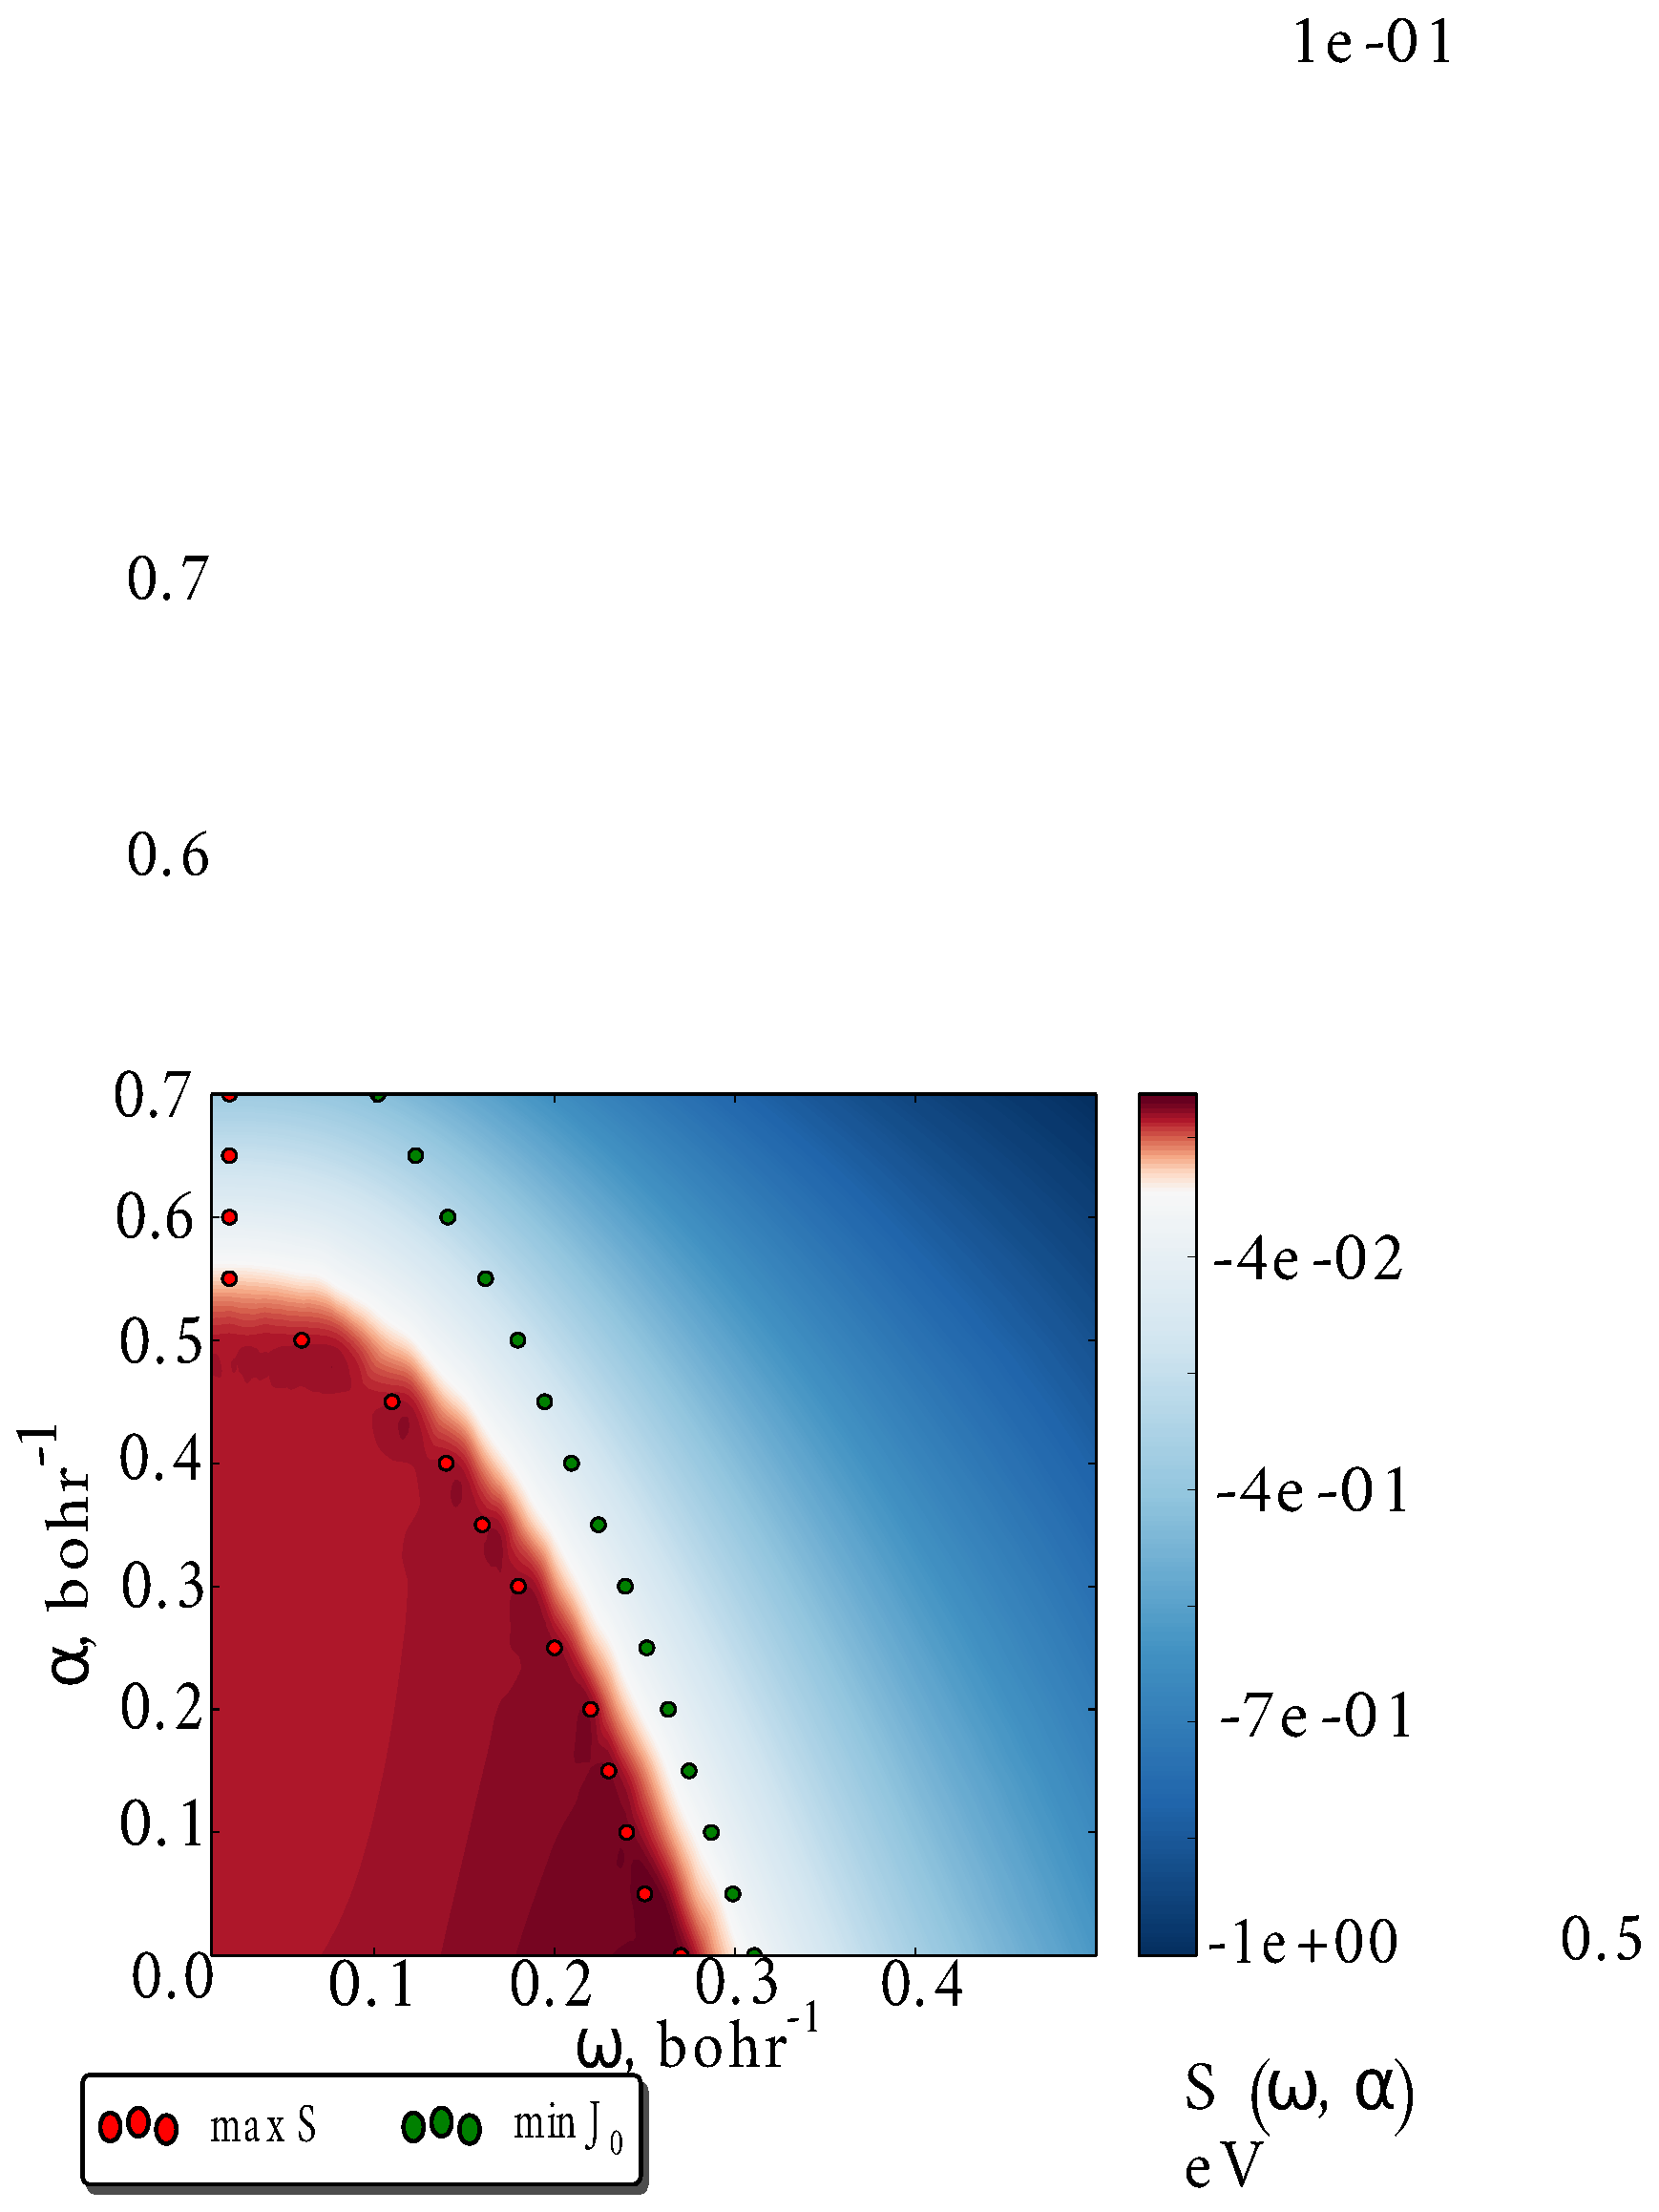
\includegraphics[width=\textwidth]{Figures/Sulphur/S8_stab_ion_cut_all}
   %\caption{deine Mudda}
   %\label{fig:SulphurStab}
%\end{figure}

%\begin{figure}
   %\includegraphics[width=\textwidth]{Figures/Sulphur/Sulphur}
%\end{figure}
%\begin{figure}
%\begin{subfigure}{0.5\textwidth}
   %\includegraphics[width=\textwidth]{Figures/Sulphur/S8_vapour}
%\end{subfigure}
%\begin{subfigure}{0.5\textwidth}
   %\includegraphics[width=\textwidth]{Figures/Sulphur/compS8}
%\end{subfigure}
%%\end{figure}


%\section{Delaunay Triangulation}
\label{app:delaunay}
The explicit setup of non-regular meshes for the use in finite element schemes is not trivial at all.
There are however schemes available, among which are the Delaunay and Voronoi tesselations which are their respective dual schemes.
Since in this thesis, only Delaunay tesselation is used, I will focus on this method and its properties only.\\
In mathematics one understands under a triangulation a connection of points to simplices.
Thereby a structure is denoted as a simplex in $n$ dimensions, if has as few vertices as possible in this dimension.
A simplex in $2D$ \textit{e.g.} is a triangle while it is in $3D$ a tetrahedron.
Moreover, a simplex is denoted as Delaunay simplex if there is a circumsphere such that no vertex is inside of this sphere.\\
A bit more intuitive acess to this scheme can be obtained via the Voronoi diagram: A Voronoi diagram splits a given volume (in $3D$) into elements using a set of points $p_i$ in this volume by assigning each point to the element of his nearest point $p_i$.
Having this tesselation, one can transform it to a set of Delaunay simplices by connecting the points $p_i$ each with their direct neighbours \cite{tetgen}.

\newpage
\section*{Selbst\"andigkeitserklaerung}
Ich versichere hiermit an Eides statt, dass ich di vorliegende Arbeit selbstst\"andig und ohne fremde Hilfe verfasst habe, keine au\ss er den von mir angegebenen Hilfsmitteln und Quellen dazu verwendet habe und die den benutzten Werken inhaltlich und w\"ortlich entnommenen Stellen als solche kenntlich gemacht habe.

\vspace{20mm}
\hfill Rostock, \date
%\printindex
\backmatter
\end{document}
